%%This is a very basic article template.
%%There is just one section and two subsections.
\documentclass[12pt]{book}

% ***********************************************************
% ******************* PHYSICS HEADER ************************
% ***********************************************************
% Version 2

\usepackage{amsmath} % AMS Math Package
\usepackage{amsthm} % Theorem Formatting
\usepackage{amssymb}	% Math symbols such as \mathbb
\usepackage{graphicx} % Allows for eps images
\usepackage{multicol} % Allows for multiple columns
\usepackage[dvips,showframe,letterpaper,margin=1.0in,left=1.5in]{geometry}
% tim included
\usepackage[pdftex,bookmarks=true]{hyperref}

\usepackage{cancel}
\usepackage{siunitx}
 % Sets margins and page size
\pagestyle{plain} % Removes page numbers
\makeatletter % Need for anything that contains an @ command 
\renewcommand{\maketitle} % Redefine maketitle to conserve space
{ \begingroup \vskip 10pt \begin{center} \large {\bf \@title}
	\vskip 10pt \large \@author \hskip 20pt \@date \end{center}
  \vskip 10pt \endgroup \setcounter{footnote}{0} }
\makeatother % End of region containing @ commands
\renewcommand{\labelenumi}{(\alph{enumi})} % Use letters for enumerate
% \DeclareMathOperator{\Sample}{Sample}
\let\vaccent=\v % rename builtin command \v{} to \vaccent{}
\renewcommand{\v}[1]{\ensuremath{\mathbf{#1}}} % for vectors
\newcommand{\gv}[1]{\ensuremath{\mbox{\boldmath$ #1 $}}} 
% for vectors of Greek letters
\newcommand{\uv}[1]{\ensuremath{\mathbf{\hat{#1}}}} % for unit vector
\newcommand{\abs}[1]{\left| #1 \right|} % for absolute value
\newcommand{\avg}[1]{\left< #1 \right>} % for average
\let\underdot=\d % rename builtin command \d{} to \underdot{}
\renewcommand{\d}[2]{\frac{d #1}{d #2}} % for derivatives
\newcommand{\dd}[2]{\frac{d^2 #1}{d #2^2}} % for double derivatives
\newcommand{\pd}[2]{\frac{\partial #1}{\partial #2}} 
% for partial derivatives
\newcommand{\pdd}[2]{\frac{\partial^2 #1}{\partial #2^2}} 
% for double partial derivatives
\newcommand{\pdc}[3]{\left( \frac{\partial #1}{\partial #2}
 \right)_{#3}} % for thermodynamic partial derivatives
\newcommand{\ket}[1]{\left| #1 \right>} % for Dirac bras
\newcommand{\bra}[1]{\left< #1 \right|} % for Dirac kets
\newcommand{\braket}[2]{\left< #1 \vphantom{#2} \right|
 \left. #2 \vphantom{#1} \right>} % for Dirac brackets
\newcommand{\matrixel}[3]{\left< #1 \vphantom{#2#3} \right|
 #2 \left| #3 \vphantom{#1#2} \right>} % for Dirac matrix elements
\newcommand{\grad}[1]{\gv{\nabla} #1} % for gradient
\let\divsymb=\div % rename builtin command \div to \divsymb
\renewcommand{\div}[1]{\gv{\nabla} \cdot #1} % for divergence
\newcommand{\curl}[1]{\gv{\nabla} \times #1} % for curl
\let\baraccent=\= % rename builtin command \= to \baraccent
\renewcommand{\=}[1]{\stackrel{#1}{=}} % for putting numbers above =
\newtheorem{prop}{Proposition}
\newtheorem{thm}{Theorem}[section]
\newtheorem{lem}[thm]{Lemma}
\theoremstyle{definition}
\newtheorem{dfn}{Definition}
\theoremstyle{remark}
\newtheorem*{rmk}{Remark}

% ***********************************************************
% ********************** END HEADER *************************
% ***********************************************************
\pagenumbering{arabic}
\numberwithin{equation}{section}
%NEW COMMANDS
\newcommand{\beqa}{\begin{eqnarray*} }
\newcommand{\eeqa}{\end{eqnarray*} }
\newcommand{\beq}{\begin{equation} }
\newcommand{\eeq}{\end{equation} }
\newcommand{\beqB}{\begin{equation*}}
\newcommand{\eeqB}{\end{equation*}}
% macros used for consistency
\newcommand{\Psibar}{\bar{\Psi}}
\newcommand{\rapidity}{\phi}
\newcommand{\TensBi}{\Sigma} %(Tensor bilinear)

%nonrelativistic wave functions
\newcommand{\phis}{\phi_S}
\newcommand{\wnr}{\phi_S}
\newcommand{\wnrb}{\phi_S^\dagger}

%nonrelativistic fields
\newcommand{\fnr}{\Psi}
\newcommand{\fnrb}{\Psi^\dagger}

%relativistic fields
\newcommand{\fr}{\Psi}
\newcommand{\frb}{\bar{\Psi} }

%spinors u, ubar
\newcommand{\sr}{u}
\newcommand{\srb}{\bar{u}}


\newcommand{\smalldot}{\cdot}
%from dirac_redo.tex
\newcommand{\sigdot}[1]{ \gv{\sigma} \hspace{-2pt} \cdot \hspace{-2pt} \v{#1} \,}
\newcommand{\sigdotg}[1]{ \gv{\sigma} \hspace{-2pt} \cdot \hspace{-2pt} \gv{#1} \,}
\newcommand{\explus}{(\sigdotg{\pi} - i\mu' \sigdot{E} )}
\newcommand{\exminus}{(\sigdotg{\pi} + i\mu' \sigdot{E} )}

\newcommand{\gradE}{\grad}


%matrix/vector/spinor shorthands
\newcommand{\spinor}[2]{ \begin{pmatrix} #1 \\ #2 \end{pmatrix} }
\newcommand{\Mblock}[4]{\begin{pmatrix} #1 & #2 \\ #3 & #4 \end{pmatrix} }

\newcommand{\Sb}{\bar{S}}

\newcommand{\A}{a}
\newcommand{\Adag}{a'}


\newcommand{\VertexEq}[2]{ \mbox{
\begin{minipage}{1.6in}
   \includegraphics[scale=0.8]{eps/#1} 
\end{minipage}
{ \large $	=	\hspace{2em} 	\large{#2} $ }
} }


\usepackage{setspace}
\doublespacing
\begin{document}


\tableofcontents

\chapter{Introduction}
We wish to calculate the gyromagnetic ratio of a particle of arbitrary spin in a loosely bound state system.  We can write down an effective Lagrangian which will capture all the necessary effects.  Our job is then to calculate the coefficients of this effective particle.  By considering the constraints which exist on the electromagnetic current in a general relativistic theory, we can obtain a simple form which holds for arbitrary spin, and then use this to fix the coefficients of the relativistic theory.

While for a particle of general spin we do not have an exact Lagrangian, we do have one for a spin-$1$ theory.  We can use this Lagrangian to perform the same calculation as above, but in an exact theory.  We derive the nonrelativistic potential first from the equations of motion, and then from diagrammatic calculations, and obtain a result that agrees with the more general calculation.  
\subsection{Description of problem}
We consider a loosely bound system two particles of arbitrary spin, and wish to calculate the correction to the gyromagnetic ratio of the particles.  So we consider the case of the two particles interacting with both each other, via a Coulomb potential, and a very weak external magnetic field.
\subsubsection{Experimental Motivation}

Talk about 


\subsubsection{Approach}
This system allows for several simplifications.  First, because the system is loosely bound all energy scales are nonrelativistic.  
%TODO details of nonrelativistic nature
Second, the magnetic field we consider is both very weak and constant.  So we can ignore all corrections which involve derivatives of the magnetic field or which are quadratic in its strength.

The approach we'll take is to first consider the electric potential as an external field acting on a single particle.  Next we can consider the bound system as a whole sitting in an external magnetic field, and take into account recoil effects.

%Discuss to what order we need to do the calculations

\subsection{Theoretical Background}

(Here we talk about existing theoretical work in this area)
\subsubsection{Spin-$1/2$}

(Here talk about the approach that works for spin 1/2, and why it breaks down in the general case.)

\subsubsection{BMT equation}

(Here discuss the BMT equation, which holds for general spin and can be used to derive the g-factor corrections)

\subsubsection{Khriplovich general spin work}
(Discuss the work Khriplovich did with general spinors.)


\chapter{NRQED}




We can construct an effective, nonrelativistic Lagrangian for a charged particle interacting with an electromagnetic field.
------
(quick outline)
Background

Construction
- Define the interaction -- physical situation and the fields involved
- enumerate building blocks
-- ($\bar{S}$ text here)
-Define order of terms
-Symmetry of terms
-Enumerating terms
-- Start by discussing how spin/position operators combine.  
-- More indices on spin operator -> higher order position space operator.
-- Make clear that there are exactly 4 orders of terms ($v^2, v^4, B, Bv^2$)
-- First construct all order unity objects
-- Construct position space terms for each order, going through number of indice	s
-- (then contracting with the order unity objects)
-- Now we have all terms in the Lagrangian
Calculation
-- section on diagrams from the Lagrangian
-- 


------


\section{Effective Field Theories}

The origin of quantum field theories lies in the search for an exact theory of nature.  At first to formulate a theory of electromagnetism which would include both relativity and quantum mechanics, and later to also account for the weak and strong forces.

For a theory to be exact, it must account for behavior at all energy scales.  The dramatic success of quantum electrodynamics (QED) as a field theory suggested that pursuing such theories was a reasonable course to chart.  In the 1950s, the predictions of QED agreed with very precise measurements of quantities such as the gyromagnetic ratio.  

However, success in formulating field theories for the other interactions was not so easy to come by.  After much frustration it became a common belief that they were not the correct tool to approach the strong or weak interactions.  While alternatives were sought, field theories found a different use in condensed matter physics.  

Here, while technically the exact theory underlying the behavior was known---that is, the microscopic interactions between particles---it was not so useful in describing the macroscopic behavior of the system.  But, an {\it effective} field theory, valid for the scale of interest could be developed. 

This approach proved fruitful in particle physics as well as condensed matter.  It was possible to formulate ``renormalizable'' theories of the weak and strong force, where the interaction was cut off at some arbitrary energy scale, and the predictions of such a theory shown to be independent of the cut-off value.  Eventually nonrenormalizable theories were also accepted, the cut-off in such theories having a physical significance.  Such theories were effective theories, capturing the behavior of a system in a particular energy regime.  While not an exact theory in themselves, they can never-the-less produce results of arbitrary accuracy in the scale of interest.

\subsection{How an effective theory works}

An effective theory acknowledges some fundamental energy scale.  Above this energy new processes and physics emerge, but below it the effective theory can capture all the interactions.  Of course the high energy physics still has some effect on the low, but it occurs as corrections to the low energy processes.  In the language of Feynman diagrams, the processes allowed at low energy can contain internal lines and loops, corrections which represent the effect of virtual particles.  Regardless of the energy of the external particles, there will still enter some corrections from all allowed processes.

The key to formulating the effective theory is to discard detailed information about these processes.  Rather, all allowed low energy processes are considered in the Lagrangian, but with coefficients that conceal the energy dependent behavior.  It is exactly the same case as say, the form factors of particles in QED.  There is a lot of complicated physics going on inside a proton, but if only low energy processes are dealt with, the exact details are hidden.  Effectively the proton will behave like a fundamental particle, and all the information about the exact theory is inside its form factors.

So the idea is this: to write down a Lagrangian which takes into account all possible processes which can occur in the regime of interest.  In front of each term will be a coefficient which may depend on the energy of the particular interaction.  Such a Lagrangian will capture the behavior of the system of interest with arbitrary precision, if the coefficients can be made known.

Now, in reality not {\it all} terms will be written down.  In a renormalizable theory there is a limit to what terms may appear, and coupling constants with negative mass dimension are not allowed.  Remember that each term in the Lagrangian must have mass dimension four, and that each field (no matter what the type) has {\it some} positive mass dimension. It becomes clear that terms involving a great number of fields are forbidden in a renormalizable theory, since their coefficient would necessarily be of negative mass dimension.

But in a theory that may be nonrenormalizable, interactions between an arbitrarily large number of fields will be possible.   And so to write a complete Lagrangian would involve an infinite number of terms.  However, one part of the above still holds true: as the number of fields in a term increases, the mass dimension of the coefficient must decrease.  This indicates a suppression of such terms by the fundamental energy scale of the problem.  Since (by the very definition) all the fields included in the effective Lagrangian have energy scales small in comparison to that fundamental cut-off scale, these terms give smaller and smaller contributions to any particular calculation.

So in practice, once the precision desired for a calculation is determined, only a finite number of terms in the effective Lagrangian need be considered.

Now, once all relevant terms are written, there will still be many undetermined coefficients left in the theory, and unlike the form of the terms, the coefficients cannot be determined {\it a priori}.  If an exact theory is known and tractable, then the coefficients can be calculated from that.  Or, just as is done for fundamental constants in an exact theory, one might simply have to take them from experiment.

\section{Nonrelativistic Quantum Electrodynamics}
One particular effective theory of interest is nonrelativistic quantum electrodynamics (NRQED).  It is a perfect example of how, even when an exact theory is known, an effective theory, especially suited for a particular energy regime, may be more practical.

The theory of atomic bound states is precisely described by QED; however, in practice calculations past the leading order can be quite tedious.  This comes about because of the interplay of several different scales; corrections can come:
\begin{itemize}
  \item from relativistic effects, corresponding to expansion in $v = (Z\alpha)$
  \item from radiative corrections, corresponding to an expansion in the coupling constant $\alpha$
  \item or from recoil corrections, an expansion in $m/M$
\end{itemize}  
Once these corrections start appearing in combination it can be quite complex to calculate and account for all effects that enter at a particular level of precision.

Using an effective theory, instead of exact QED, is useful because it already separates out the relativistic effects.  All the information from the exact theory is preserved, but rather than struggling to reconcile a nonrelativistic problem with a relativistic theory, we first craft a theory particularly suited to the problem.

There are two particularly important features this effective theory will have that make it nonrelativistic, in addition to an explicit cut-off.  First, rather than demanding manifest Lorentz symmetry, only the nonrelativistic Galilean symmetry will be required.  Second, it will be a theory without an explicit anti-particle.  This is because, without access to energies approaching the particle mass, there is no way for an anti-particle to be produced. (Of course if a system like positronium is to be studied both particle and anti-particle must be included in the theory, but as {\it separate} fields.)

With these principles in mind the effective Lagrangian for NRQED can be written down, for the case of a fermion like the electron:  

\beq \label{eq:nrLfermion}
\mathcal{L}_{NRQED} =  \fnrb \Bigg\{
		iD_0 +  \frac{\v{D}^2}{2m}  + 	\frac{\v{D}^4}{8m^2}
		 + c_F \frac{e}{2m} \gv{\sigma} \cdot \v{B} 
		+ c_D \frac{e \div \v{E}}{8m^2} 
	 + c_S \frac{ i e \gv{\sigma} \cdot(\v{D} \times \v{E} - \v{E} \times \v{D}}{8m^2}
		\Bigg \} \fnr
\eeq
Here are included only the terms involving two powers of the electron field.

The coefficients themselves are fixed by calculating some processes in the relativistic theory at a particular energy.  For instance, scattering off an external field will fix all those terms containing a single external field above, by comparing to the same calculation (at the same energy) done with the NRQED Lagrangian.  

However, it is key while doing so to establish a strict relationship between the single particle fields of NRQED and the relativistic fields (including particle and anti-particle) of QED.  This relationship may be found through the Foldy-Wouthyusen transformation.
\subsection{The NRQED Lagrangian}

We want to construct an effective Lagrangian in the nonrelativistic limit.  Our goal is to calculate the leading order corrections to the $g$-factor, which are corrections of order $\alpha^2$.  To this end, we need terms in the effective nonrelativistic Lagrangian which are equivalent corrections.

\subsubsection{Order of terms}
%TODO Discussion of energy scales --  possibly move this into introduction, since it applies to each calculation
We consider constant, infinitesimal external magnetic fields, so we need only consider terms linear in $\v{B}$.

The velocity of the particles in our bound state system will be $v \sim \alpha$.

The electric field we consider is the Coulomb field, so $e\Phi \sim m Z\alpha^2 \sim mv^2$, and $eE \sim m^2v^3$.

Each derivative of the electric field will add an additional factor of $mv$, so the operator $\v{D}$ can be taken to be of this order.

We need to keep terms up to order $mv^4$ and $\frac{B}{m} v^2$ in order to calculate the $g$-factor to the necessary precision.  We include $mv^4$ terms so we can be sure that there are no effects entering from second-order perturbation theory.



%TODO insert qualifications on external field
\subsubsection{Constraints on the form of the Lagrangian}
The Lagrangian is constrained to obey several symmetries.  It must be invariant under the symmetries of parity and time reversal.  It must also be invariant under Galilean transformations.  The Lagrangian must also be Hermitian, and gauge invariant.

What are the gauge invariant building blocks we can use to construct this Lagrangian?  We have the external fields $\v{E}$ and $\v{B}$, the spin operators $\v{S}$, and the long derivative $\v{D} = \v{\partial} - i e\v{A}$.  The fields should always be accompanied by the charge $e$ of the particle.

When considering the case of higher spin particles, we might consider terms quadratic and above in spin operators.  For a particle of spin $s$, there must be $(2s+1)^2$ independent hermitian operators.  We can span this set of operators by considering products of up to $2s$ spin matrices which are symmetric and traceless in every vector index.  For example, for spin-$1$ we have quadratic, in addition to $I$ and $S_i$, five independent structures of the form $ S_i S_j + S_j S_i + \delta_{ij} \v{S}$.

We also have the scalar $D_0$, however, we need only include a single such term because we insist on having only one power of the time derivative.

To consider possible terms, we need to know how each of the above behave under the discrete transformations and Hermitian conjugate.  The signs under these transformations are listed in the table below.  (Also included is the imaginary number $i$.)


\begin{tabular}{l|c|ccc}
& Order	&	P	&	T	&	$\dagger$	\\
\hline
$eE_i$	&$m^2v^3$	&	-	& 	+	&	+		\\
$eB_i$	&$m^2v^2$	&	+	&   -	&	+		\\
$D_i$		& mv	&	-	&	+	&	-		\\
$D_0$		& mv	&	+	&	-	&	-		\\
$S_i$		& 1		&	+	&	-	&	+		\\
$i$		& 1		&	+	&	-	&	-		\\
\end{tabular}

\subsubsection{Allowed terms}
Our strategy in cataloguing terms will be to first list all the combinations of $E$, $B$ and $D$ which might be allowed at a particular order, to consider the various ways of contracting these vectors, and finally to eliminate terms which do not obey the proper symmetries.  We can always make a particular combination Hermitian, and get the proper behavior under time reversal by adding a factor of $i$, but parity will kill several terms.  Note that of the structures we can contract with, all are even under parity.

%List objects with which we can contract the vector fields

We can also insist that the Lagrangian have the expected form in the absence of external fields, which eliminates terms like $\bar{S}_{ij}D_i D_j$.  The leading order terms should be of order $mv^2$ or $\frac{eB}{m}$.  Combinations of the correct order are:
\begin{itemize}
  \item The single $D_0$ term.  To have the correct transformation properties this should be $iD_0$.
  \item The kinetic $\v{D}^2$ term, which must be simply $\frac{\v{D}^2}{2m}$
  \item A term with a single power of $B_i$.  The only way to contract this is with the spin matrix, so the term will have the form $\frac{e}{m} \v{S} \cdot \v{B}$
\end{itemize}
All these terms are Hermitian in themselves.

So, the allowed terms at this order are:
\[
	iD_0, \frac{\v{D}^2}{m}, \frac{e}{m} \v{S} \cdot \v{B}
\]

The first two terms have their coefficients fixed, while we wish to honestly calculate the factor before the last.

%TODO check signs and other factors for consistency
\beq \label{eq:nrLFirstOrder}
	\mathcal{L}_{NRQED} = \fnrb \Bigg\{ iD_0 +  \frac{\v{D}^2}{2m}  +  c_F \frac{e}{m} \v{S} \cdot \v{B}\Bigg \} \fnr
\eeq

Are there any terms of order $mv^3$ or $\frac{B}{m}v$ allowed?  Possible combinations are:
\begin{itemize}
  \item Three powers of D: $D_i D_j D_k$.  However, this is odd under parity, and so not allowed.  
  \item A term with both the derivative and magnetic field: $D_i B_j$.  Again, this is odd under parity and so forbidden.
  \item A single power of $E$.  Again, odd under parity.
\end{itemize}
So, all such terms are foribdden by consideration of parity.

Next we consider terms of order $mv^4$.
\begin{itemize}
  \item Four powers of D: fixed by the kinetic term to be $\frac{\v{D}^2}{8m^3}$
  \item One power of $E_i$ and one of $D_j$.  This combination is even under parity and odd under Hermitian conjugate.  There are three ways of contracting these two fields.
  \begin{itemize}
  		\item	With the delta function.  The allowed Hermitian term is then $\delta_{ij}(D_i E_j - E_j D_i)$.
  		\item	With the combination $i\epsilon_{ijk} S_k$.  The allowed term is $i\epsilon_{ijk}(D_i E_j S_k + S_k E_j D_i)$.
  		\item 	With the quadratic spin structure $Q_{ij}$: $ Q_{ij} ( D_i E_j - E_j D_i)$.
  \end{itemize}
\end{itemize}

In the Lagrangian we'll write these as:
\beq \label{eq:nrLv4}
	\mathcal{L}_{mv^4} = \fnrb \Bigg\{
		\frac{\v{D}^4}{8m^2}
		+ c_D \frac{e (\v{D} \cdot \v{E} - \v{E} \cdot \v{D})}{8m^2} 
		+ c_Q \frac{eQ_{ij}(D_i E_j - E_i D_j)}{8m^2}
		+ c_S \frac{ i e \v{S} \cdot(\v{D} \times \v{E} - \v{E} \times \v{D}}{8m^2} \Bigg \} \fnr
\eeq


Terms of order $\frac{B}{m} v^2$.  The only allowed combination is $D_i D_j B_k$.  We can contract two indices with each other and the third with a spin matrix in three different ways:
\begin{itemize}
	\item $(\v{S} \cdot \v{B}) \v{D}^2 +  \v{D}^2 (\v{S} \cdot \v{B})$
	\item $S_i D_j B_i D_j$
	\item $S_i (D_i B_j D_j + D_j B_j D_i)$
\end{itemize}
We can also contract all indices with a cubic spin structure:
\begin{itemize}
  \item $\bar{S}_{ijk} (D_i D_j B_k + B_k D_j D_i)$
  \item $\bar{S}_{ijk} D_i B_j D_k$
\end{itemize}

In the Lagrangian we'll write these as:
\beq \label{eq:nrLBv2} \begin{split}
	\mathcal{L}_{Bv^2} = &
		\fnrb \Bigg\{
			c_{W1} \frac{ e \v{D}^2 \v{S} \cdot \v{B} + \v{S} \cdot \v{B} \v{D}^2 }{8m^3}
			- c_{W2} \frac{e D_i (\v{S} \cdot \v{B}) D_i}{4m^3}
			+c_{p'p} \frac{ e [ (\v{S}\cdot \v{D})(\v{B} \cdot \v{D}) + (\v{B} \cdot \v{D})(\v{S}\cdot \v{D})]}{8m^3}
\\ &		+ c_{T_1} \frac{ e \bar{S}_{ijk} (D_i D_j B_k + B_k D_j D_i)}{8m^3}
		+ c_{T_2} \frac{ e \bar{S}_{ijk} D_i B_j D_k }{8m^3} \Bigg \} \fnr
\end{split}\eeq


\subsubsection{Full Lagrangian}
The full Lagrangian we consider is then:

\beq \label{eq:nrLFull}
\begin{split}
\mathcal{L}_{NRQED} = & \fnrb \Bigg\{
		iD_0 +  \frac{\v{D}^2}{2m}  + 	\frac{\v{D}^4}{8m^2}
		 + c_F \frac{e}{m} \v{S} \cdot \v{B}
		+ c_D \frac{e (\v{D} \cdot \v{E} - \v{E} \cdot \v{D})}{8m^2} 
		+ c_Q \frac{eQ_{ij}(D_i E_j - E_i D_j)}{8m^2}
\\	& + c_S \frac{ i e \v{S} \cdot(\v{D} \times \v{E} - \v{E} \times \v{D}}{8m^2}
		+ c_{W1} \frac{ e \v{D}^2 \v{S} \cdot \v{B} + \v{S} \cdot \v{B} \v{D}^2 }{8m^3}
		- c_{W2} \frac{e D_i (\v{S} \cdot \v{B}) D_i}{4m^3}
\\	&		+c_{p'p} \frac{ e [ (\v{S}\cdot \v{D})(\v{B} \cdot \v{D}) + (\v{B} \cdot \v{D})(\v{S}\cdot \v{D})]}{8m^3}
 	+ c_{T_1} \frac{ e \bar{S}_{ijk} (D_i D_j B_k + B_k D_j D_i)}{8m^3}
		+ c_{T_2} \frac{ e \bar{S}_{ijk} D_i B_j D_k }{8m^3} 
		\Bigg \} \fnr
\end{split}
\eeq


One of the features of this Lagrangian is that every coefficient is fixed by the one-photon interaction.  Although some terms might represent two-photon interactions, they are terms like $\v{S} \cdot \v{A} \times \v{E}$, whose coefficient is fixed by the gauge-invariant term $\v{S} \cdot \v{D} \times \v{E}$.  This in turn means that we can calculate the corrections to the $g$-factor by considering only one-photon interactions.






\subsection{Scattering off external field in NRQED}
We can write down those terms in the NRQED Lagrangian which have one power of the external field.  This set of terms will not, by themselves, be gauge invariant. If, for example, a coefficient exists before a term with both one and two powers of $A$, we'll want to make sure we get the same result in both calculations.  We'll add a superscript to the coefficient to keep track of this: so below we write $c^1_S$.

In writing the expansion of terms like $\v{D}^4$ it is convenient to use anticommutators.
\small
\beqa
\mathcal{L}_A &=& \fnrb (  -eA_0- ie  \frac{ \{\nabla_i, A_i \} }{2m} -ie \frac{ \{\grad^2, \{\nabla_i, A_i \}  \} }{8m^3} 
		+ c_F e \frac{\v{S} \smalldot \v{B}} {2m}   	
		+ c_D \frac{ e(\v{\grad} \smalldot \v{E} - \v{E} \smalldot \v{\grad} ) }{8m^2}	
		+ c_Q \frac{e Q_{ij} (\nabla_i E_j - E_i \nabla_j) }{8m^2}	
	\\&&	+ c^{1}_S \frac{ ie \v{S} \smalldot ( \v{\grad} \times \v{E} - \v{E} \times \v{\grad} )}{8m^2}
		+ c_{W_1} \frac{ e [ \v{\grad}^2 (\v{S} \smalldot \v{B} ) + (\v{S} \smalldot \v{B} ) \v{\grad}^2] }{8m^3}	
		- c_{W_2} \frac{ e \nabla^i (\v{S} \smalldot \v{B} ) \nabla^i }{4m^3}
		+ c_{p'p} \frac{ e [ (\v{S} \smalldot \v{\grad}) (\v{B} \smalldot \v{\grad}) + (\v{B} \smalldot \v{\grad})(\v{S} \smalldot \v{\grad}) }{8m^3} \big )\fnr
\eeqa
\normalsize

We want to calculate from this a particular process: scattering off an external field, with incoming momentum $\v{p}$, outgoing $\v{p'}$, and $\v{q} = \v{p'} - \v{p}$.  There is one diagram associated with each term above, but the total amplitude is just going to be the sum of all these one-photon vertices.  These of course can just be read off directly from the Lagrangian: we replace the fields $\Psi$ with the spinors $\phi$, and any operator $\grad$ acting will become $i\v{p}$ if it acts on the right, $i\v{p'}$ if it is to the left.

We can simplify some expressions involving $\grad$ and $\v{E}$:
Because $Q_{ij}$ is symmetric:
\[
	 Q_{ij} (\nabla_i E_j - E_i \nabla_j ) = Q_{ij} [\nabla_i, E_j] = Q_{ij} (\partial_i E_j)
\]

And because $E_i = -\partial_i \Phi$
\[
	\v{\grad} \times \v{E} - \v{E} \times \v{\grad} =  - 2 \v{E} \times \v{\grad}
\]
And also use that
\[
\v{\grad} \smalldot \v{E} - \v{E} \smalldot \v{\grad} = (\partial_i E_i)
\]


Now we can write down the scattering amplitude for scattering off the external field, before we apply any assumptions about the particular process.
\beqa
	iM &=&
		ie\wnrb \Bigg( - A_0 +    \frac{ \v{A} \cdot (\v{p} + \v{p'}) }{2m} 
		- \frac{  \v{A} \cdot (\v{p} + \v{p'}) \v{p}^2 + \v{p'}^2 \v{A} \cdot (\v{p} + \v{p'}) }{8m^3} 
	\\&&	+ c_F  \frac{\v{S} \smalldot \v{B}} {2m}   	
		+ c_D \frac{ ( \partial_i E_i ) }{8m^2}	
		+ c_Q \frac{Q_{ij}  ( \partial_i E_j ) }{8m^2}	
		+ c^{1}_S \frac{  \v{E} \times \v{p} }{4m^2}
	\\&&	- c_{W_1}  \frac{  (\v{S} \smalldot \v{B} ) (\v{p}^2 + \v{p'}^2)  }{8m^3}
		+ c_{W_2} \frac{  (\v{S} \smalldot \v{B} ) (\v{p} \cdot \v{p'}) }{4m^3}
		-  c_{p'p} \frac{  (\v{S} \smalldot \v{p'}) (\v{B} \smalldot \v{p}) + (\v{B} \smalldot \v{p'}) (\v{S} \smalldot \v{p}) }{8m^3} \Bigg )\wnr
\eeqa

The above can be simplified somewhat.  We choose our gauge such that $\nabla_i A_i = 0$.  If we specify elastic scattering then kinematics dictate that $\v{p'}^2 = \v{p}^2$.   Finally, if we consider $\v{B}$ constant, the $c_W$ terms become indistinguishable, since $[ \nabla_i, B_j] = 0$.    (It is only this last assumption that costs us any information.)  Then the scattering amplitude, as calculated from $\mathcal{L}_{NRQED}$, is:

\beq 
\begin{split} \label{eq:nrqedScatter}
	iM =&
		ie\wnrb \Bigg(  -A_0 +  \frac{ \v{A} \cdot \v{p} }{m} - \frac{  (\v{A} \cdot \v{p}) \v{p}^2   }{2m^3} 
		+ c_F  \frac{\v{S} \smalldot \v{B}} {2m}   	
		+ c_D \frac{ ( \partial_i E_i ) }{8m^2}	
		+ c_Q \frac{ Q_{ij} ( \partial_i E_j ) }{8m^2}	
	\\&	+ c^{1}_S \frac{  \v{E} \times \v{p} }{4m^2}
		- (c_{W_1} -c_{W_2}) \frac{   (\v{S} \smalldot \v{B} ) \v{p}^2  }{4m^3}	
		-  c_{p'p} \frac{   (\v{S} \smalldot \v{p}) (\v{B} \smalldot \v{p})  }{4m^3} \Bigg )\wnr 
\end{split}
\eeq
\chapter{Spin one-half}

\section{Structure of spin one-half theory}

The goal is to obtain a nonrelativistic theory from the relativistic.  To that end it'll help to have a clear understanding of the structure of the two theories.

\subsection{Relativistic framework for spin one-half}
In the relativistic theory, the electrons are part of a fermion field that also includes the positron anti-particle.  Since both are spin-1/2, each has two spin orientations.  There are, then, a total of four degrees of freedom. 

The relativistic Lagrangian for the fermion fields is
\beqa
\mathcal{L} &=&	
	\bar{\Psi}(i \partial \cdot \gamma - e A \cdot \gamma - m)\Psi  - \frac{1}{4} F_{\mu\nu} F^{\mu\nu}
\eeqa

The fermion fields are $\Psi$, the photon field is $A$.   $m$ is the particle's mass, and $e$ the electron's charge.  The $\gamma$ matrices mix the different components.  %TODO better explanation of gamma matrices

It will be convenient to work in a representation which already suggests the nonrelativistic behavior.  At low momenta, it should be expected that the free electron and positron fields act approximately as independent fields.  This is exactly the case for the Dirac representation.   In the rest frame, a free particle can be said to be definitively an electron or positron, and in the Dirac representation these correspond to the upper and lower parts of the bispinor.  

In this representation, the gamma matrices are written
\beq
	\gamma^0 = \Mblock{1}{0}{0}{-1}
\eeq

\beq
	\gamma^i = \Mblock{0}{\sigma_i}{-\sigma_i}{0}
\eeq	




The gamma matrices by themselves do not form a complete basis for this space.  To find such a basis products of the matrices can be considered.  It will make sense to consider combinations such that bilinears are Hermitian.  
 

There is the identity --- such bilinears transform as a scalar.

Symmetric combinations are not considered because $\{ \gamma^\mu, \gamma^\nu \}= g^{\mu\nu}$.  The antisymmetric combinations are explicitly
 \beqa
	  {[\gamma^0, \gamma^i]}
		&=&  2 \gamma^0 \gamma^i = \begin{pmatrix}	0 & 2\sigma_i \\ 2\sigma_i & 0\end{pmatrix}	\\
	  {[\gamma^i, \gamma^j ]}
		&=&	 \begin{pmatrix}	-2i\epsilon_{ijk}\sigma_k & 0 \\ 0 & -2i\epsilon_{ijk}\sigma_k\end{pmatrix}
\eeqa
Using these a tensor like structure arises:
\beq
	\sigma^{\mu \nu} = i \frac{1}{2} [ \gamma^\mu, \gamma^\nu]	%defined as in Peskin p.50
\eeq

The specific form in the Dirac representation is
\beq
	\sigma^{ij} = \frac{i}{2} [ \gamma^i, \gamma^j] 
		= \epsilon_{ijk} \Mblock{\sigma_k}{0}{0}{\sigma_k}
\eeq
\beq
	\sigma^{0i} = i \gamma^0 \gamma^i 
			= \Mblock{0}{i \sigma_i}{i \sigma_i}{0}
\eeq

The product of each gamma matrix in turn gives a pseudo-scalar:
\beq
	\gamma^5 = i \gamma^0 \gamma^1 \gamma^2 \gamma^3 = \Mblock{0}{1}{1}{0}
\eeq
 
 The product of $\gamma^5$ and $\gamma^\mu$ gives a pseudo-vector
 \beq
 	\gamma^5 \gamma^\mu 
 \eeq
 

\beq
	\sr = \begin{pmatrix} \eta \\ \chi \end{pmatrix}
\eeq
 
\subsection{Nonrelativistic framework for spin one-half}





\beqa
	\eta &=& \left( 1  - \frac{\v{p}^2}{8m^2} \right ) w	\\
	\chi &=& 	\frac{ \gv{\sigma} \cdot \v{p}}{2m} \left(1 - \frac{3\v{p}^2}{8m^2} \right ) w	\\
\eeqa



 \section{Foldy-Wouthyusen approach}
 
The goal is to derive a nonrelativistic Hamiltonian or Lagrangian starting from relativistic theory.  (Having obtained one, we can easily obtain the other, of course.)  One method is to take the relativistic equations of motion and use them to obtain a Schrodinger like equation.

The starting point is the relativistic equations of motion, which can come from the Lagrangian of the relativistic theory.  Those equations can then be written in terms of the noncovariant quantities that appear in the nonrelativistic theory.  In doing so, the energy of the particle will now explicitly appear.

The relativistic theory will contain not only the particle of interest (the electron) but also its anti-particle (the positron.)  The nonrelativistic theory should contain only the electron.  Before obtaining an expression for the nonrelativistic Hamiltonian it will be necessary to somehow disentangle the two fields.  This is impossible in the general case, but as long as the energy and momenta in question are nonrelativistic, can be accomplished to any desired order.

Formally this is accomplished by the Foldy-Wouthyusen transformation, the result of which is that all operators are diagonal, the coupling between the particle and anti-particle suppressed to which ever order is desired.  However, practically the same result can be obtained by examining the normalisation of the two theory's particles.  By demanding that the Schrodinger like wave functions are appropriately normalized, the relationship between relativistic and nonrelativistic spinors can be established.

The result of this procedure will be an equation for the energy of the electron, accurate at some order in the nonrelativistic expansion.  However, it will not perfectly replicate the predictions of the high energy theory.  Unlike the process of NRQED, it does not truly incorporate the high energy sector of the theory.



\subsection{Equations of motion}

To reestablish the problem considered, the system to be examined is an electron placed in a loosely bound system with another charged particle, subject to an infinitesimal and constant magnetic field.  There will be, because of the bound system, an electric field acting on the electron as well as the external magnetic field.  When recoil effects are ignored, the electric field can just be taken as given.

The corrections to the gyromagnetic ratio of the electron are to be established.  There are two small scales that appear in the problem, the velocity $v$ of the electron and the infinitesimally small magnetic field $eB$.  The precision desired requires terms of up to order $mv^4$ and $ (e/m)Bv^2$.

The starting point will be the relativistic Lagrangian of Dirac.  However, remember that the technique to be used simply ignores behavior introduced by the high energy sector of the theory, even if it might effect the low energy behavior.  One such effect is corrections to the free gyromagnetic ratio of the electron, which first arise when one loop diagrams are considered.  Without such corrections the $g$-factor will be exactly $g=2$.

Knowing that there will actually be bound-state corrections proportional to $g-2$, it is necessary to somehow include this anomalous term.  The way to do so is to introduce a new local interaction into the Lagrangian, coming from the high energy radiative corrections which dress the electron vertex.  The Lagrangian to be used is, then
\beqa
\mathcal{L} &=&	
	\bar{\Psi}(\cancel{D} - m)\Psi + \frac{1}{2} \mu' \bar{\Psi} \sigma^{\mu\nu}F_{\mu\nu} \Psi	
\eeqa
%TODO check \mu_0
$\mu'$ is the correction to the classical moment $\mu_0 = \frac{e}{2m}$, and is equal to $(g-2)/2 \mu_0$.  $D$ is the long derivative $\partial + ieA$.


From this Lagrangian the equations of motion of the particle may be obtained from the Euler-Lagrange method.  The Euler-Lagrange equation is
\beq
\pd{ \mathcal{L}}{{\bar{\Psi} } } - \partial_\mu \frac{\partial \mathcal{L}} {\partial (\partial_\mu {\bar{\Psi})} } 
	= 0	
\eeq

In the Lagrangian above, we can consider that all differential operators act only on the right field $\Psi$.  (This freedom of choice comes from being able to rewrite the Lagrangian through integration by parts, without changing its physical meaning.)  So the second term in the Euler-Lagrange equation can be ignored, and after differentiating with respect to $\bar{\Psi}$ the following equation is obtained:
\beq
	(i\cancel{D} - m + \frac{1}{2} \mu'  \sigma^{\mu\nu}F_{\mu\nu} )\Psi = 0	
\eeq
Writing explicitly in terms of the $\gamma$ matrices, this is
\beq \label{eq:Sh:eom}
	\left( (i\partial_\mu- eA_\mu)\gamma^\mu -m + i\mu' \frac{1}{4}[ \gamma^\mu, \gamma^\nu]F_{\mu\nu} \right) \Psi
		=0
\eeq
This equation of motion is invariant under Lorentz transformations.  It is written in terms of the Dirac bispinor $\Psi$, external fields $A_\mu$ and $F_{\mu\nu}$, and the gamma matrices.  To apply in to a nonrelativistic problem, the very first step will be to rewrite it in terms of the sorts of quantities that appear in that domain: three-vectors and scalars.

The scalars that appear will be $\partial_0= \partial_t$ and $A_0 = \Phi$.  The external fields $\v{E}$ and $\v{B}$ will appear explicitly, while the vector field $\v{A}$ will appear in the gauge-invariant operator $\gv{\pi} = \v{p} - e\v{A}$.  The gamma matrices can be written in terms of the Pauli spin matrices $\gv{\sigma}$.  Finally, the bispinor will be written in terms of its upper and lower components.

Of the terms that appear in \eqref{eq:Sh:eom}, all except the last are trivial to write in this manner.  To deal with that last term, the antisymmetric tensor $\sigma^{\mu\nu} =  \frac{1}{2}[\gamma^\mu, \gamma^\nu]$ needs to be written explicitly.

Using the antisymmetry of $\sigma^{\mu\nu} \equiv $, and that we deal with time-independent fields: %TODO fix sigma
\beqa
	F_{\mu\nu} \sigma^{\mu\nu} &=& F_{i}\sigma^{ij} - F_{0i}\sigma^{0i} 	- F_{i0}\sigma^{i0} +F_{00}\sigma^{00}	\\
		&=&	F_{ij} \sigma^{ij} -2F_{0i} \sigma^{0i}	\\
		&=&	2 \partial_i A_j \sigma^{ij} - 2\partial_i \Phi \sigma^{0i}	\\
		&=&	-2i \begin{pmatrix} \sigdot{B} & 0 \\ 0 & \sigdot{B}\end{pmatrix}	
			-2 \begin{pmatrix} 0 & \sigdot{E} \\ \sigdot{E} & 0 \end{pmatrix}	
\eeqa

So far the discussion has been in position space.  To work out the nonrelativistic form it will be easier to talk about the equations of motion directly in terms of energy and momentum.  So replace $i\partial_t$ with $p_0$, and $i\partial_i$ with $p_i$.  Likewise, replace the gauge invariant derivative  $iD_i = \pi_i = p_i - eA_i$.

A solution of definite momentum $p$ to the equation is written in terms of upper and lower components
\beq
	u = \begin{pmatrix} \eta \\ \chi \end{pmatrix}
\eeq


With these considerations, the \eqref{eq:Sh:eom} can be rewritten acting explicitly on the bispinor.

\beq \label{eq:Sh:matrixEOM}
	\left\{
		\begin{pmatrix}
			p_0 - e\Phi	- m &	0	\\
			0	&	-p_0 + e\Phi - m	\\
		\end{pmatrix}
		+
		\begin{pmatrix}	0 & -\sigdotg{\pi} \\  \sigdotg{\pi} & 0 \end{pmatrix} 
		+\mu'\left [
			\begin{pmatrix}
				\sigdot{B} & 0 \\ 0 & \sigdot{B}
			\end{pmatrix}
			-i \begin{pmatrix}
				0 & \sigdot{E} \\ \sigdot{E} & 0
			\end{pmatrix}
		\right ] 
	\right\} \begin{pmatrix} \eta \\ \chi \end{pmatrix}
		= 0
\eeq
This gives rise to exact coupled equations for $\eta$ and $\chi$.  So far this is in principle the same as the relativistic equation, only the form in which it is written is non covariant.

\subsection{Nonrelativistic limit}

The particle under consideration is a nonrelativistic electron.  Roughly, the expectation is that $\eta$ corresponds to the electron field and $\chi$ to that of the positron.  The off-diagonal terms in the equation above represent some sort of mixing between the electron and positron: the electron wave function still has some small positron component, that decreases as momentum is decreased.    The off diagonal component that does {\it not} vanish at 0 momentum is proportional to $\mu'$, the term introduced to account for a high-energy process.

The upshot is that although the equation above is really a set of coupled equations for $\eta$ and $\chi$, $\chi$ will be small compared to $\eta$ --- the very leading order diagonal term will indicate that $\chi \sim \sigdotg{\pi} \eta$.

Because the off diagonal terms are small, the set of coupled equations may be solved perturbatively.  The particular quantity of interest is the nonrelativistic energy of the particle $\epsilon = p_0 - m$.  For a free particle, this would be
\beq
	\epsilon = p_0 - m \approx \frac{\v{p}^2}{2m} + \frac{\v{p}^4}{8m^3} + \mathcal{O}\left (\frac{\v{p}^6}{m^5} \right )
\eeq  

In order to perform this perturbative analysis the order of various terms needs to be established.  It's evident that at leading order $\epsilon \sim mv^2$.  From earlier analysis,   $\Phi\sim mv^2$, $\v{\pi} \sim mv$, and $\v{E} \sim m^2v^3$.

First, find an expression for $\chi$ in terms of $\eta$.  The second of the set of equations represented by \eqref{eq:Sh:matrixEOM} is
\beq
	(-p_0 + e\Phi - m) \chi + \sigdotg{\pi} \eta + \mu'( \sigdot{B} \chi - i \sigdot{E}  \eta)
\eeq
Writing $p_0 = \epsilon + m$, and grouping terms, the result is that
\beq
	\left( \epsilon + 2m - \mu' \sigdot{B} \right ) \chi = \left( \sigdotg{\pi} - i\sigdot{E} \right) \eta	
\eeq
It is necessary now to approximate $\chi$ in terms of $\eta$.  Because $\epsilon$ and $\abs{B}$ are smaller than $m$, and only second order terms are needed for the final result:
\beq
	\chi \approx	\frac{1}{2m} \left ( 1- \frac{\epsilon - e\Phi - \mu' \sigdot{B}}{2m} \right ) (\sigdotg{\pi} - i\mu' \sigdot{E} )\phi
\eeq

With this expression $\chi$ may be eliminated from the first of the set of equations (at least at the necessary order).  The resulting equation will only involve $\eta$, and so may be used to solve for energy $\epsilon$ of  $\eta$.

The original equation is
\beq
	(p_0 - e\Phi - m) \eta - \sigdotg{\pi} \chi + \mu'( \sigdot{B}\eta  - i \sigdot{E} \chi ) 
\eeq
So again using $p_0 - m = \epsilon$
\beq
	\epsilon \eta 	= (e\Phi - \mu' \sigdot{B} )\eta + (\sigdot{E} + \sigdotg{\pi}) \chi	
\eeq
Now the expression for $\chi$ in terms of $\eta$ may be used.
\beq
 	\epsilon \eta \approx (e\Phi - \mu' \sigdot{B} )\eta + (\sigdot{E} + \sigdotg{\pi})  \frac{1}{2m} \left ( 1- \frac{\epsilon - e\Phi - \mu' \sigdot{B}}{2m} \right ) (\sigdotg{\pi} - i\mu' \sigdot{E} )\eta 
\eeq				
 
Writing the $1/m$ and $1/m^2$ terms separately:
\beq
\begin{split}				\epsilon \eta		\approx& \left \{
		e\Phi - \mu' \sigdot{B} + \frac{ \exminus \explus}{2m}	\right. \\
		& \left. +\frac{1}{4m^2} \exminus (\mu' \sigdot{B} - [\epsilon - e\Phi]) \explus 	
	\right \} \eta	
\end{split}
\eeq

Several of the terms are of too high order to consider.  A term with both $E$ and $B$, for instance, will be of higher order than $(e/m)\abs{B} v^2$.  Likewise, a term of $E \Phi$ or $E \epsilon$ is also too small.  Dropping all such:
\beq
	\epsilon \eta \approx \left \{
				e\Phi - \mu' \sigdot{B} + \frac{(\sigdotg{\pi})^2 - i\mu' [\sigdotg{\pi}, \sigdot{E}]}{2m}
				+\frac{1}{4m^2} \sigdotg{\pi} (\mu' \sigdot{B} - [\epsilon - e\Phi]) \sigdotg{\pi} 
			\right \} \eta
\eeq
This is an expression for the energy $\epsilon$ of the particle, in terms of operators.  This will yield the nonrelativistic Hamiltonian.  There is still some manipulation required, though, because the right hand side also contains $\epsilon$.  But since the leading order terms don't, it may be perturbatively solved for.  (The above expression could be simplified somewhat, using the properties of $\sigma$ matrices for instance, but for now it is more convenient to write it compactly.)

To that end, the Hamiltonian can be split into leading order and second order terms.  The leading order will be of $mv^2$ and $(e/m)B$, while the next order will be suppressed by an additional factor of $v^2$.  Because the magnetic field is infinitesimally small no $B^2$ terms are needed. 
 Since the leading order term in H is $\mathcal{O}(mv^2)$, this suggests we split it into two parts: $H = H_0 + H_1 +\mathcal{O}(mv^6, (e/m) B v^4)$, where $H_1$ consists of only second order terms.
\beqa
	\hat{H_0} 
			&=&  e\Phi - \mu' \sigdot{B} + \frac{ (\sigdotg{\pi})^2}{2m}	\\
	\hat{H_1} 
			&=& -\frac{i\mu'}{2m}  [\sigdotg{\pi}, \sigdot{E}]
				+\frac{1}{4m^2} \sigdotg{\pi} (\mu' \sigdot{B} - [\epsilon - e\Phi]) \sigdotg{\pi} 
\eeqa
$H_1$ contains $\epsilon$, along with other terms of total order $mv^2$.  So to eliminate $\epsilon$ from $H_1$ it'll only be necessary to find it to leading order.
\beqa
	\epsilon \eta
			&=& \left(\hat{H_0} + \mathcal{O}(mv^4) \right)\eta 										\\
			&\approx& \left(e\Phi - \mu' \sigdot{B} + \frac{ (\sigdotg{\pi})^2}{2m}	\right) \eta			
\eeqa
The operators on the right hand side, operating on $\eta$, produce $\epsilon$.  The combination actually needed is $\sigdotg{\pi} \epsilon \sigdotg{\pi}$.  To that end, start with $\sigdotg{\pi}^2 \epsilon$ and use commutation relations.
\beqa
	(\sigdotg{\pi})^2 (\epsilon - e\Phi) \eta		
			&=&	(\sigdotg{\pi})^2 \left ( \frac{(\sigdotg{\pi})^2}{2m}- \mu' \sigdot{B} \right )	\eta	\\
	\sigdotg{\pi} (\epsilon - e\Phi) \sigdotg{\pi}\eta
			&=&	\left( \frac{(\sigdotg{\pi})^4}{2m} 
				- \mu' (\sigdotg{\pi})^2 \sigdot{B} 
				- \sigdotg{\pi}[e\Phi, \sigdotg{\pi}]\right ) \eta
\eeqa
With this $\epsilon$ is eliminated, leaving:
\beq
	\hat{H}_1	=
		-\frac{i\mu'}{2m}  [\sigdotg{\pi}, \sigdot{E}]
		+\frac{1}{4m^2}\left(
			\mu' \sigdotg{\pi} \sigdot{B} \sigdotg{\pi}
			- \frac{(\sigdotg{\pi})^4}{2m} 
			+ \mu' (\sigdotg{\pi})^2 \sigdot{B} 
			+ \sigdotg{\pi}[e\Phi, \sigdotg{\pi}]
		\right)
\eeq
Some terms couple $A$ and $B$; they can be dropped.  Some simplification of the structures involving $\sigma$ matrices can be done.  To start with, simplify $(\sigdotg{\pi})^2$.
\beq
	(\sigdotg{\pi})^2 = \sigma_i \sigma_j \pi_i \pi_j = \pi^2 - i\epsilon_{ijk} \pi_i \pi_j \sigma_k
\eeq
Since $\v{p} \times \v{p} = \v{A} \times \v{A} = 0$, from $\gv{\pi} \times \gv{\pi}$ only the cross terms survive:
\beq
	(\sigdotg{\pi})^2 = \pi^2 - i e \epsilon_{ijk}(p_i A_j - A_i p_j) = \pi^2 - e \sigdot{B}
\eeq
Looking at the terms $\mu' \sigdotg{\pi} \sigdot{B} \sigdotg{\pi} + \mu' (\sigdotg{\pi})^2 \sigdot{B}$, they contain an anticommutator involving $B$ and $p$.  Because the magnetic field is assumed to be constant, $p$ and $B$ commute, so: 
\beqa
\{ \sigdot{B}, \sigdot{p} \}	&=&		B_i p_j \{\sigma_i, \sigma_j\}	\\
		&=&	2\v{B}\cdot \v{p}	
\eeqa
The commutator of $\Phi$ and a derivative operator should give the electric field $E$:
\beq
	[ \Phi, \sigdotg{\pi} ]	= [ \Phi, p_i] \sigma_i = -iE_i \sigma_i = -i\sigdot{E} 
\eeq
Using these identities, the Hamiltonian can be expressed as:
\beq
	\hat{H_0} 
			=  e\Phi - \mu' \sigdot{B} + \frac{ \pi^2}{2m} - \frac{e}{2m} \sigdot{B}	\\
\eeq
\beq
	\hat{H}_1	=
		- \frac{\pi^4}{8m^3}  
		+ e\frac{p^2}{4m^3} \sigdot{B}
		-i \frac{\sigdotg{\pi} \sigdot{E}}{4m^2} 
		+ \mu' \left(	
			\frac{ \sigdot{p} \v{B}\cdot \v{p} }{2m^2}
			-\frac{i[\sigdotg{\pi}, \sigdot{E}]}{2m} 
		\right )
\eeq
There are still some simplifications that can be made to terms quadratic in $\sigma$, but it'll be more convenient for now to keep $H$ written as is.

\subsection{Foldy-Wouthyusen Transform}

To find a complete description of a single nonrelativistic particle in normal quantum mechanics, we must work in a basis where the lower component $\chi$ is truly negligible, at least at the desired order.  While there exists a formal technique for finding this Foldy-Wouthyusen transformation, for our purposes we can simply demand that the wave function after transformation $\phis = (1 + \Delta)\eta$ obeys $\langle \phis, \phis \rangle = 1$.  This follows from the necessity of probability conservation.

To find the necessary transformation, we can use the relativistic current density, and demand it equal that of the nonrelativistic Schrodinger-like wave functions.   Using the expression for $\chi$ in terms of $\eta$:
\beqa
	\int d^3x (\eta^\dagger \eta + \chi^\dagger \chi) 	
		&=& \int d^3x 	\left[ \eta^\dagger \phi + \left (\frac{\sigdotg{\pi}}{2m} \phi \right)^\dagger
										   \left (\frac{\sigdotg{\pi}}{2m} \eta \right)
						\right ]	\\
		&=& \int d^3x 	\eta^\dagger \left[ 1 + \frac{ (\sigdotg{\pi})^2 }{4m^2} \right ] \eta
\eeqa
Since we know that $\langle \phis, \phis \rangle=1$ this shows that if $\eta = \left( 1 - \frac{ (\sigdotg{\pi})^2 }{8m^2} \right )\phis$, the current conservation works out correctly.


We now need to find the form of $\hat{H}$ after this transformation.  For now work with the general form:
\beq
	\epsilon \eta = (\hat{H}_0 + \hat{H}_1) \eta 
\eeq
After changing to the Schrodinger like wave functions, this becomes:
\beq
	\epsilon \left (1 - \frac{(\sigdotg{\pi})^2}{8m^2} \right )\phi_S =  (\hat{H}_0 + \hat{H}_1) \left(1 - \frac{(\sigdotg{\pi})^2}{8m^2}\right)\phi_S 
\eeq
To the order needed the inverse of $1 + \sigdotg{\pi}^2 / 8m^2 $ is just $1 - \sigdotg{\pi}^2 / 8m^2 $, so eliminating that on the left hand side gives:
\beq
	\epsilon \phi_S =  (1 + \frac{(\sigdotg{\pi})^2}{8m^2})(\hat{H}_0 + \hat{H}_1) (1 - \frac{(\sigdotg{\pi})^2}{8m^2})\phi_S
\eeq
Since $H_1$ is already second order, these further corrections don't involve it directly.  Expressing the result as a commutator:
\beq
	\epsilon \phi_S = \left (  \hat{H}_0 + \frac{1}{8m^2}[(\sigdotg{\pi})^2, \hat{H}_0] + \hat{H}_1 \right )\phi_S 
\eeq
So under the FW transformation, the leading order term is unchanged, and the second order term is:
\beq
	 \hat{H}_1 \to \hat{H}_1' = \hat{H}_1 + \frac{1}{8m^2}[(\sigdotg{\pi})^2, \hat{H}_0]
\eeq

The final step is to simplify the commutator $ [(\sigdotg{\pi})^2, \hat{H}_0] $.
  
\beq [(\sigdotg{\pi})^2, \hat{H}_0] = [(\sigdotg{\pi})^2, e\Phi - \mu' \sigdot{B} + \frac {(\sigdotg{\pi})^2}{2m}] \eeq

Obviously $(\sigdotg{\pi})^2$ commutes with itself, so that term vanishes.  Since $\sigdot{B}$ is constant, that commutator will also disappear.  Writing $\sigdotg{\pi}$ as shown earlier:
$$[(\sigdotg{\pi})^2, \mu' \sigdot{B}] =[\pi^2 - e \sigdot{B}, \mu'\sigdot{B}] = 0 $$


The non-trivial part is the commutation of the derivative operators with the electric potential $\Phi$. 
\beqa
[(\sigdotg{\pi})^2, \hat{H}_0] &=& [(\sigdotg{\pi})^2, e\Phi] \\
		&=&	e( \sigdotg{\pi}[\sigdotg{\pi},  \Phi] + [\sigdotg{\pi},  \Phi]\sigdotg{\pi}) \\
		&=&	i e( \sigdotg{\pi} \sigdot{E} + \sigdot{E} \sigdotg{\pi} ) \\
\eeqa
So, writing down the new $H_1'$:
\beqa
\hat{H}_1' 
	&=&  \hat{H}_1 + \frac{i e}{8m^2}( \sigdotg{\pi} \sigdot{E} + \sigdot{E} \sigdotg{\pi} )	\\
	&=&	 -\frac{\pi^4}{8m^3} + e \frac{p^2}{4m^3}\sigdot{B} - \frac{ie}{8m^2}[\sigdot{E},\sigdotg{\pi}]
		 + \mu' \left( \frac{ (\sigdot{p}) (B \cdot p) }{2m^2} - \frac{i}{2m}[\sigdot{E},\sigdotg{\pi}] \right)
\eeqa

\subsection*{Nonrelativistic Hamiltonian}
From the relativistic equations of motion, a nonrelativistic Hamiltonian was defined in terms of Schrodinger-like wave functions that conserve probability.  The final result may now be written down.  For comparison with other work, rather than writing in terms of $\mu'$, it will be written in terms of the gyromagnetic ratio $g$.  Because terms proportional to $g-2$ may enter seperately, it is convenient to express all $g$ dependent terms as linear combinations of $g$ and $g-2$. 

So the entire Hamiltonian, using $\mu' = \frac{g-2}{2}\mu_0 = \frac{g-2}{2}\frac{e}{2m} $, is:
\begin{eqnarray*}
H	&=&
		e\Phi  + \frac{ \pi^2}{2m} -\frac{\pi^4}{8m^3} - (1 + \frac{g-2}{2})\frac{e}{2m} \sigdot{B}	\\
	&&
		 + e \frac{p^2}{4m^3}\sigdot{B} + \frac{ie}{8m^2}(1 + (g-2))[\sigdot{E},\sigdotg{\pi}]
		 + (g-2) \frac{e}{2m}  \frac{ (\sigdot{p}) (\v{B} \cdot \v{p}) }{4m^2}  	\\
	&=&
		e\Phi  + \frac{ \pi^2}{2m} -\frac{\pi^4}{8m^3} 
	\\&&
		- \frac{e}{2m} \left\{
			\frac{g}{2}\sigdot{B} - \frac{p^2}{2m^2}\sigdot{B}
			- (g-2) \frac{ (\sigdot{p}) (\v{B} \cdot \v{p}) }{4m^2} 
			+(g-1) \gv{\sigma} \cdot (\v{E} \times \gv{\pi})
		\right \}	\\
	&=&
		e\Phi  + \frac{ \pi^2}{2m} -\frac{\pi^4}{8m^3} 
	\\&&
		- \frac{e}{2m} \left\{
			\frac{g}{2} \left( 1 - \frac{p^2}{2m^2} \right) \sigdot{B} + \frac{g-2}{2} \frac{p^2}{2m^2}\sigdot{B}
			- \frac{g-2}{2} \frac{ (\sigdot{p}) (\v	{B} \cdot \v{p}) }{2m^2} 
			+\left(\frac{g}{2} + \frac{g-2}{2}\right) \gv{\sigma} \cdot (\v{E} \times \gv{\pi})
		\right \}	\\	
\end{eqnarray*}

			


 
 
 

%skeleton of calculation
\section{Method of NRQED}
%define spinors and structures
Instead of starting from the relativistic equations of motion and rewriting them in the form of a Schrodinger like equation, the method of NRQED can be employed.  The nonrelativistic Lagrangian can be written in the most general way, but ignoring all possible terms that will have too small a contribution to calculations.  The coefficients before each term will be unknown, but there is a straightforward method of fixing them.

Within the realm of NRQEDs validity, it should produce the same predictions as QED.  The same physical process can be calculated in both frameworks, and then the results compared.  The calculation in QED will then fix the coefficients in NRQED.  In comparing the two calculations it will be necessary to write the QED results nonrelativisitcally, in the same manner as was done for the equation of motion.
%TODO mention free vs. nonfree spinors?

For spin one-half, up to the order desired, the form of the NRQED Lagrangian involving two fermion fields has been derived in the previous chapter.  It is
\beq \label{eq:Sh:nrL-2f}
\begin{split}
\mathcal{L}_{NRQED} = & \fnrb \Bigg\{
		iD_0 +  \frac{\v{D}^2}{2m}  + 	\frac{\v{D}^4}{8m^2}
		 + c_F \frac{e}{m} \v{S} \cdot \v{B}
		+ c_D \frac{e (\v{D} \cdot \v{E} - \v{E} \cdot \v{D})}{8m^2} 
\\	& + c_S \frac{ i e \v{S} \cdot(\v{D} \times \v{E} - \v{E} \times \v{D}}{8m^2}
		+ c_{W1} \frac{ e \v{D}^2 \v{S} \cdot \v{B} + \v{S} \cdot \v{B} \v{D}^2 }{8m^3}
		- c_{W2} \frac{e D_i (\v{S} \cdot \v{B}) D_i}{4m^3}
\\	&		+c_{p'p} \frac{ e [ (\v{S}\cdot \v{D})(\v{B} \cdot \v{D}) + (\v{B} \cdot \v{D})(\v{S}\cdot \v{D})]}{8m^3}
		\Bigg \} \fnr
\end{split}
\eeq
Each term contains two fermion fields, and zero, one or two powers of the photon field.  Terms with a different number of photon fields, of course, correspond to different physical processes.  But because gauge invariance is a necessary feature of the theory, the coefficients of many terms involving the photon field are constrained to be the same as that of terms with a smaller number of such fields.  For instance, the gauge invariant term $\v{D}^2/(2m)$ is: 
\beq	
	\frac{\v{D}^2}{2m} = \frac{ \grad^2 - i e (\grad \cdot \v{A} + e \v{A} \cdot \grad ) - e^2 \v{A}^2 }{2m}
\eeq
The first term above, containing $\grad^2$, is a purely kinetic term.  The other two represent interactions with one or two photon fields.  To fix these coefficients, two physical processes could be calculated and compared with the QED results, but in the end they must have the same coefficient as guaranteed by gauge invariance.

Obviously not every term goes this same way.  The term with $\v{S} \cdot \v{B}$, for instance, is in and of itself gauge-invariant, and so there is no option but to calculate it from a process involving a single photon.  For the necessary terms appearing in the above Lagrangian, it would suffice to consider just the one photon processes.  However, since in principle some of the interesting coefficients could be calculated from two photon diagrams, this also will be done. 

To fix these terms, some physical process must be chosen.  For the one photon terms, scattering off an external field will be calculated.  For the two photon terms, Compton scattering will be used.

\subsection{Calculation of electron scattering off external field in QED}
%First form
To fix all the terms in the NRQED Lagrangian which have a single power of the photon field, it suffices to calculate the scattering of an electron off an external field, as represented (in QED) by the diagram

   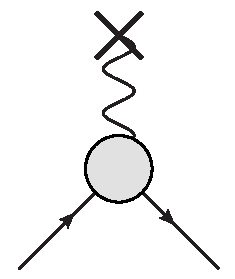
\includegraphics[scale=0.8]{eps/blob-wave} 
	%TODO add additional diagrams


The leading order contributions (in QED) to this interaction come from the fundamental electron vertex.  There are radiative corrections to this process, starting at the one loop order.  In principle, such calculations (up to some desired order in $\alpha$) should be included in the QED calculation.  

However, it turns out that the actual {\it form} of the interaction is highly constrained by the symmetries of the theory.  No matter the source of contributions to the vertex, their effects can be incorporated into two coefficients or form factors.  The NRQED coefficients can then be written in terms of these form factors, which can later be calculated to whatever precision is necessary.  

The first symmetry that constrains the interaction is that it must be invariant under Lorentz transformations.  Since every term involves the photon field $A_\mu$ and has external fermion legs, then the interaction must be proportional to the general form:
\beq
	A_\mu \srb(p') \Gamma^\mu(p', p) \sr(p) 
\eeq 	
and $\srb(p') \Gamma^\mu(p', p) \sr(p) $ must transform as a Lorentz vector.  If it did not, the whole would not be Lorentz invariant.  To leading order $\Gamma^\mu = \gamma^\mu$, since the fundamental vertex is just that.  The corrections, whatever the exact details of the processes which produce them, can only depend on the momenta $p$ and $p'$, in addition to constants $m$ and $e$, and such structures as may act upon the spinors.

A basis for such structures is known, with well defined Lorentz transformations.  That gives scalar, vector, tensor, pseudo-vector, and pseudoscalar terms.  From the momenta in the problem can be constructed scalar and vector quantities.  What symmetries control the allowed terms?

In addition to proper Lorentz invariance, it is necessary that the interaction as a whole preserve parity.  Since $A$ is a vector, the term $\srb \Gamma^\mu \sr$ must also behave as a vector under parity transformations.  And there is no Lorentz invariant combination of external momenta that can be written that is not even under parity.   Because of this, there can be no contribution from the pseudovector and pseudoscalar bilinears.

The vector bilinear $\srb \gamma^\mu \sr$ already has the correct transformation properties.  From the scalar bilinear $\srb \sr$, a vector can be constructed by adjoining a single power of the momentum.  (As, for example, $p^\mu \srb \sr$.)  And after contracting one index of the tensor with a momentum vector, it will also behave as a vector.

The momenta terms available are $p$ and $p'$.  However, the terms constructed from them are not independent, because each must separately obey current conservation.  So whatever terms go into $\Gamma^\mu$, $q_\mu \srb \Gamma^\mu \sr = 0$.  The unique scalar term will be
\beq
	\frac{p^\mu + p'^\mu}{2m} \srb \sr
\eeq     
which vanishes because $(p'+p) \cdot (p'-p) = p'^2 - p^2 = m^2- m^2=0$.

The unique tensor term allowed will be
\beq
	\frac{q_\nu}{2m} \srb \sigma^{\mu\nu} \sr
\eeq
which conserves current because $\sigma^{\mu\nu}$ is antisymmetric.  So from these considerations, the general form of the vertex will have three terms, each with a momentum dependant coefficient:
\beq \label{eq:Sh:Gamma}
	\srb \Gamma^\mu \sr 
		= 	c_1(p, p') \frac{p^\mu + p'^\mu}{2m} \srb \sr
			+ c_2(p, p') \srb \gamma^\mu \sr
			+ c_3(p, p') \frac{q_\mu}{2m} \srb \sigma^{\mu\nu} \sr
\eeq

However, there is one more consideration.  From the Dirac equation can be derived the Gordon identity, which relates these three terms:
\beq \label{eq:Sh:gordon}
	\srb \gamma^\mu \sr = \srb \left( \frac{p^\mu + p'^\mu }{2m} + \frac{i \sigma^{\mu\nu}q_\nu}{2m} \right ) \sr
\eeq

With this, any one of the terms in \eqref{eq:Sh:Gamma} can be rewritten as some combination of the other two, and its coefficient effectively absorbed into the other two.  To write down the most general form of the vertex, one need only choose two of the three terms.  Which two to choose might depend on the nature of the calculation; at any rate, there are always three paths to go down.

In the calculation of scattering off an external field an agnostic approach will be taken at first.  The scattering amplitude is some combination of the three bilinears.  The goal is to rewrite the scattering amplitude in nonrelativistic language.  So, each bilinear in turn will be rewritten in this manner.

The vertex can be written in each of three ways.  The form factors will be defined with respect to the particular combination of $\gamma^\mu$ and $\sigma^{\mu\nu}$ terms.

\beq
	\Gamma^\mu = \gamma^\mu F_1(q^2) + i \frac{\sigma^{\mu\nu}q_\nu}{2m} F_2 (q^2)
\eeq

Using the Gordon identity to write this in terms of the scalar and vector bilinears, the result is
\beq
	\Gamma^\mu = \gamma^\mu [F_1(q^2) + F_2(q^2) ]  -  \frac{p^\mu  + p'^\mu }{2m}F_2 (q^2)
\eeq

And writing in terms of the scalar and tensor:
\beq
	\Gamma^\mu = \frac{p^\mu  + p'^\mu }{2m} F_1(q^2) + i \frac{\sigma^{\mu\nu}q_\nu}{2m} [F_1(q^2) + F_2(q^2) ] 
\eeq

%TODO move this section up a bit?
The momentum dependence can be uniquely written in terms of $q^2$.  The factors must be Lorentz invariant, so only such combinations of momenta can be considered.  From the momenta $p$ and $p'$, only three such quantities can be constructed.  But since the external fermions are on mass-shell, $p^2 = p'^2 = m^2$.  That leaves only $p \cdot p' = m^2 + p \cdot q$, and this can be related to $q^2$ by noting that since $p^2 = p'^2$,
\beq
	p^2 = p^2 + 2p\cdot q + q^2  \to q^2 = -\frac{1}{2} p \cdot q
\eeq


Given that there exist these three ways to write the vertex, there are three ways to perform the calculation.  The scattering amplitude will have the form
\beq	
	i M = 	A_\mu \srb(p') \Gamma^\mu(p', p) \sr(p) 
\eeq
and no matter which way $\Gamma^\mu$ is written, a nonrelativistic expansion in terms of $\phis$ will be needed.  For now an agnostic approach will be taken, and the expressions for each of the three possible bilinears found.


\subsubsection{Nonrelativistic expressions for the bilinears}
To compare with the NRQED scattering amplitude, everything needs to be written with consistent language.  We start with the relativistic bilinears, each of which behaves like a four vector, and appears in the amplitude dotted with the external field $A$.  Any dot products $a \cdot b$ should instead be written as $a_0 b_0 - \v{a} \cdot \v{b}$.  To this end, it might be necessary to treat the spatial and time-like components of the four-vector bilinears separately.

The bispinors $u$ will be first written in terms of upper and lower components $\eta$, $\chi$, and then in terms of the nonrelativistic wave spinors $w$.  The relationship between the two sets are
\beqa
	\eta(p) &=& \left( 1 - \frac{\v{p}^2}{8m^2} \right ) w(p)	\\
	\chi(p)	&=& \frac{ \sigdot{p} }{2m} \left(1  - \frac{3\v{p}^2}{8m^2} \right ) w(p)
\eeqa
In writing in terms of the upper and lower components,  the explicit expressions of the $\gamma$ matrices, as well as $\sigma^{\mu\nu}$ will be needed.  

Of course the above expressions for the spinors in terms of $w$ is approximate.  In the NRQED Lagrangian, the terms we wish to fix involve $A_0$ with up to two powers of momentum (such as $\grad \cdot \v{E}$), and $A_i$ with up to three (as in $\sigdot{B} \v{p}^2$).  Because only the case of a constant magnetic field is needed, in any term which will explicitly contain $B$ higher derivatives may be ignored.  Throwing away unneeded terms, whatever is left can be used to calculate the scattering amplitude and compare with NRQED.

This same general procedure will be followed for each of the bilinears.

\paragraph{Scalar bilinear:}
Start with the first bilinear, a scalar coupled with a momentum four-vector.  Rewrite it in terms of $\eta$ and $\chi$.
\beq
	(p + p')^\mu \srb \sr  = (p + p')^\mu \left( \eta^\dagger \eta - \chi^\dagger \chi \right ) 
\eeq
Now express in terms of $w$
\beq
	= (p + p')^\mu \left \{
		w^\dagger \left( 1 - \frac{ \v{p'}^2}{8m^2} \right )  \left( 1 - \frac{ \v{p}^2}{8m^2} \right ) w
		- w^\dagger \left( \frac{ \gv{\sigma} \cdot \v{p'}}{2m} \frac{ \gv{\sigma} \cdot \v{p}}{2m} \right ) w \right \}
\eeq 
And finally drop terms beyond the order that we need.
\beq
	= (p + p')^\mu w^\dagger \left( 
		1 -  \frac{ \v{p}^2 + \v{p'}^2}{8m^2} - \frac{ \gv{\sigma} \cdot \v{p'} \gv{\sigma} \cdot \v{p} }{4m^2} 
		\right ) w
\eeq
Simplifying $\sigdot{p'} \sigdot{p} = \v{p} \cdot \v{p'} + i\gv{\sigma} \cdot \v{q} \times \v{p}$.
\beq \label{eq:Sh:Si}
	(p + p')^\mu \srb \sr  = (p + p')^\mu w^\dagger \left( 
		1 -  \frac{ \v{p}^2  +2 \v{p} \cdot \v{p'} +  \v{p'}}{8m^2} - \frac{i\gv{\sigma} \cdot \v{q} \times \v{p} }{4m^2} 
		\right ) w
\eeq

The spatial part is straightforward, but the time-like part is 
\beq
	(p + p')^0 \srb \sr  = (p + p')_0 w^\dagger \left( 
		1 -  \frac{ \v{p}^2  +2 \v{p} \cdot \v{p'} +  \v{p'}^2 }{8m^2} - \frac{i\gv{\sigma} \cdot \v{q} \times \v{p} }{4m^2} 
		\right ) w
\eeq
Approximating the relativistic energies gives $p_0 = m + \v{p}^2 / (2m) $.  So
\beq
	p_0 + p'_0 \approx 2m + \frac{ \v{p}^2 + \v{p'}^2 }{2m} = 2m\left( 1 +  \frac{ \v{p}^2 + \v{p'}^2 }{4m^2} \right )
\eeq
Then using this correction to the leading order term
\beq
	(p + p')^0 \srb \sr  = 2m  w^\dagger \left( 
		1 +  \frac{ \v{p}^2   - 2 \v{p} \cdot \v{p'} +  \v{p'} }{8m^2} - \frac{i\gv{\sigma} \cdot \v{q} \times \v{p} }{4m^2} 
		\right ) w
\eeq
\beq \label{eq:Sh:S0}
	(p + p')^0 \srb \sr  \approx 2m  w^\dagger \left( 
		1 +  \frac{ \v{q}^2 }{8m^2} - \frac{i\gv{\sigma} \cdot \v{q} \times \v{p} }{4m^2} 
		\right ) w
\eeq


\paragraph{Vector bilinear:}
For the term $\srb \gamma^\mu \sr$ it'll be necessary to treat the spatial/time-like indices separately, since they have different spinor structure.

The time-like part is:
\beq
	\srb \gamma^0 u = u^\dagger u
\eeq
which in terms of $\eta$ and $\chi$ is just
\beq
	= \eta^\dagger \eta + \chi^\dagger \chi 
\eeq
Then rewritten with $w$
\beq
	= 	w^\dagger \left( 1 - \frac{ \v{p'}^2}{8m^2} \right )  \left( 1 - \frac{ \v{p}^2}{8m^2} \right ) w
		+ w^\dagger \left( \frac{ \gv{\sigma} \cdot \v{p'}}{2m} \frac{ \gv{\sigma} \cdot \v{p}}{2m} \right ) w 
\eeq
Which is, at the order needed
\beq
	=	 w^\dagger \left( 
		1 -  \frac{ \v{p}^2 + \v{p'}^2}{8m^2} + \frac{ \gv{\sigma} \cdot \v{p'} \gv{\sigma} \cdot \v{p} }{4m^2} 
		\right ) w
\eeq
Simplifying the last term, using $\sigma_i \sigma_j = \delta_{ij} + i\epsilon_{ijk}\sigma_k$, gives
\beq \label{eq:Sh:V0}
	\srb \gamma^0 u = 
			w^\dagger \left( 
		1 -  \frac{ \v{q}^2 }{8m^2} + \frac{i \gv{\sigma} \cdot \v{q} \times \v{p} }{4m^2} 
		\right ) w
\eeq





The spatial part is
\beq
	\srb \gamma^i \sr = \sr^\dagger \gamma^0 \gamma^i \sr
\eeq
writing the matrices explicitly
\beq
	= \srb^\dagger \begin{pmatrix}
		0 & \sigma_i \\ \sigma_i & 0 		
	\end{pmatrix} \sr
\eeq
which in terms of spinors is
\beq
	= \eta^\dagger \sigma_i \chi + \chi^\dagger \sigma_i \eta
\eeq
Replacing the spinors with $w$ gives
\beq
	= w^\dagger \left\{
		\left( 1 - \frac{ \v{p'}^2}{8m^2}   \right ) \frac{ \sigma_i \sigdot{p} }{2m} \left( 1 - \frac{3\v{p}^2}{8m^2} \right )
			+ \left( 1 - \frac{ 3\v{p'}^2}{8m^2} \right )  \frac{  \sigdot{p'} \sigma_i }{2m} \left( 1 - \frac{\v{p}^2}{8m^2} \right )
	\right\} w
\eeq
Using $\v{p'}^2 = \v{p}^2$ gives
\beq
	= w^\dagger \left\{
		\frac{ \sigma_i \sigdot{p}  + \sigdot{p'} \sigma_i }{2m} \left( 1 -\frac{ \v{p}^2}{2m^2} \right )
	\right\} w
\eeq
Then $\sigma_i \sigma_j = \delta_{ij} + i\epsilon_{ijk} \sigma_k$
\beq
	= w^\dagger \left\{
		\frac{ p_i + \epsilon_{ijk} p_j \sigma_k + p'_i  + \epsilon_{jik} p'_j \sigma_k }{2m} \left( 1 -\frac{ \v{p}^2}{2m^2} \right )
	\right\} w
\eeq
So finally
\beq \label{eq:Sh:Vi}
	\srb \gamma^i \sr  = w^\dagger \left\{
		\frac{ p_i + p'_i - \epsilon_{ijk} q_j \sigma_k }{2m} \left( 1 -\frac{ \v{p}^2}{2m^2} \right )
	\right\} w
\eeq



\paragraph{Tensor term:}
The tensor term is subject to an additional simplification.  Because the process under considering is elastic scattering off an external static field, terms involving $q_0$ can be dropped.  Under this approximation $q_\nu \sigma^{\mu\nu} \approx  q_j \sigma^{\mu j}$.

Dealing first with the case where $\mu=i$, write the tensor structure explicitly as a matrix:  
\beq
	\srb  \frac{i}{2m} q_j \sigma^{ij} \sr 
		=  \frac{i \epsilon_{ijk} q_j}{2m} \srb \Mblock{\sigma_k}{0}{0}{\sigma_k} \sr
\eeq
Write in terms of spinors
\beq
	= \frac{i \epsilon_{ijk} q_j}{2m} \left( \eta^\dagger \sigma_k \eta - \chi^\dagger \sigma_k \chi \right )
\eeq
And then in terms of $w$
\beq
	= \frac{i \epsilon_{ijk} q_j}{2m} w^\dagger \left \{
		\left( 1 - \frac{\v{p'}^2}{8m^2} \right ) \sigma_k \left( 1 - \frac{\v{p'}^2}{8m^2} \right )- \frac{ \gv{\sigma} \cdot \v{p'} \sigma_k \gv{\sigma} \cdot \v{p} }{4m^2} w
	\right \}
\eeq
There now appears a term with a triple product of $\sigma$ matrices.  That can be simplified with the following expression:
\beq
	\sigma_a \sigma_b \sigma_c = \sigma_a (\delta_{bc} + i\epsilon_{bcd}\sigma_d)
		=	\sigma_a \delta_{bc} - \sigma_b \delta_{ca} + \sigma_c \delta_{ab} + i \epsilon_{abc}	
\eeq
Using that identity, 
\beq
	\srb  \frac{i}{2m} q_j \sigma^{ij} \sr 
		= \frac{i \epsilon_{ijk} q_j}{2m} w^\dagger \left \{
			\sigma_k \left( 1 - \frac{\v{p'}^2  + \v{p}^2}{8m^2} \right ) - \frac{ \gv{\sigma} \cdot (\v{p} + \v{p'})p_k - \sigma_k \v{p} \cdot \v{p'} + i \epsilon_{akc} q_a p_c }{4m^2} 
		\right \} w 
\eeq

This can be further simplified by combining the like terms $\sigma_k (\v{p'}^2 + \v{p}^2 ) - 2 \sigma_k \v{p} \cdot \v{p'} = \sigma_k \v{q}^2$.
\beq
	\srb  \frac{i}{2m} q_j \sigma^{ij} \sr 
		= \frac{i \epsilon_{ijk} q_j}{2m} w^\dagger \left \{
			\sigma_k \left( 1 - \frac{\v{q}^2}{8m^2} \right ) - \frac{ \gv{\sigma} \cdot (\v{p} + \v{p'})p_k + i \epsilon_{akc} q_a p_c }{4m^2} 
		\right \} w 
\eeq
Now it is necessary to consider exactly what derivatives of the field $A_i$ are to be kept.  The assumption is that $B$ is constant and so $\partial_i B_j = 0$.  Contracted with $A_i$ above, $\epsilon_{ijk} A_i q_j \sim B_k$.  So besides the leading factor, no terms with $q$ are needed.  Applying this simplification,
\beq \label{eq:Sh:Ti}
	\srb  \frac{i}{2m} q_j \sigma^{ij} \sr 
		= \frac{i \epsilon_{ijk} q_j}{2m} w^\dagger \left \{
			\sigma_k - \frac{ \gv{\sigma} \cdot \v{p} p_k  }{2m^2} 
		\right \} w 
\eeq






The case with $\mu=0$ goes as follows.
\beq
	\srb  \frac{i}{2m} q_j \sigma^{0j} \sr
		=	 - \frac{q_j}{2m} \srb \gamma^0 \gamma^j \sr 		
 		=  - \frac{q_j}{2m} \sr^\dagger \gamma^j \sr
\eeq
Explicitly in matrix form 
\beq
	 = - \frac{q_j}{2m} \sr^\dagger \Mblock{0}{\sigma_j}{\sigma_j}{0} \sr 
\eeq
 Written in terms of spinors, and Galilean three-vector $q^j= -q_j$.
 \beq
 	= \frac{q^j}{2m}  \left( \eta^\dagger \sigma_j \chi - \chi^\dagger \sigma_j \eta \right )
 \eeq
 And then in terms of $w$:
\beq
	=  \frac{q^j}{2m}  w^\dagger \left \{
		\left(1 - \frac{\v{p'}^2}{8m^2} \right )  \frac{ \sigma_j \gv{\sigma} \cdot \v{p} }{2m} \left(1 - \frac{3\v{p}^2}{8m^2} \right )
		- \left(1 - \frac{3 \v{p'}^2}{8m^2} \right ) \frac{\gv{\sigma} \cdot \v{p'} \sigma_j  }{2m} \left(1 - \frac{\v{p}^2}{8m^2} \right )
	\right \} w
\eeq

This bilinear is contracted with $A_0$, and so actually, only terms involving two additional powers of momenta need be kept.
\beq
	=  \frac{q^j}{2m}  w^\dagger \left \{
		  \frac{ \sigma_j \gv{\sigma} \cdot \v{p} }{2m} 
		-  \frac{\gv{\sigma} \cdot \v{p'} \sigma_j  }{2m} 
	\right \} w
\eeq
or simplifying using the commutator of $\sigma$ matrices
\beq 
	=   \frac{q^j}{2m}  w^\dagger \left \{
		\frac{ 2 i\epsilon_{jik} p_i \sigma_k  - q_i - i\epsilon_{ijk} q_j \sigma_k }{2m} 
	\right \} w
\eeq
One term above vanishes because of symmetry
\beq \label{eq:Sh:T0}
\srb  \frac{i}{2m} q_j \sigma^{0j} \sr
	=  -  w^\dagger \left \{
			\frac{  \v{q}^2  }{4m^2} 
			- \frac{  i\gv{\sigma} \cdot \v{q} \times \v{p}   }{2m^2} 
	\right \} w
\eeq


% Start of comparison
\paragraph{Full vertex}

Now that the three bilinears have been calculated, the complete scattering amplitude can be written down.  Each of the three forms should prove equivalent.  To simplify comparison, the coupling to $A_0$ and $A_i$ can be treated separately.

The first has $	\Gamma^\mu = \gamma^\mu F_1(q^2) + i \frac{\sigma^{\mu\nu}q_\nu}{2m} F_2 (q^2)$.  Using \eqref{eq:Sh:V0} and \eqref{eq:Sh:T0}
\beq
	A_0 \srb  \Gamma^0 \sr = 
		A_0 F_1   w^\dagger \left( 
		1 -  \frac{ \v{q}^2 }{8m^2} + \frac{i \gv{\sigma} \cdot \v{q} \times \v{p} }{4m^2} 
		\right ) w
		- A_0 F_2 w^\dagger \left \{
			\frac{  \v{q}^2  }{4m^2} 
			- \frac{  i\gv{\sigma} \cdot \v{q} \times \v{p}   }{2m^2} 
	\right \} w
\eeq
The second is	$\Gamma^\mu = \gamma^\mu [F_1(q^2) + F_2(q^2) ]  -  \frac{p^\mu  + p'^\mu }{2m}F_2 (q^2)$.  Using \eqref{eq:Sh:V0} and \eqref{eq:Sh:S0}.
\beq
	A_0 \srb  \Gamma^0 \sr = 
		A_0 (F_1 + F_2)   w^\dagger \left( 
		1 -  \frac{ \v{q}^2 }{8m^2} + \frac{i \gv{\sigma} \cdot \v{q} \times \v{p} }{4m^2} 
		\right ) w
		- A_0 F_2   w^\dagger \left( 
		1 +  \frac{ \v{q}^2 }{8m^2} - \frac{i\gv{\sigma} \cdot \v{q} \times \v{p} }{4m^2} 
		\right ) w
\eeq
The third combination is $	\Gamma^\mu = \frac{p^\mu  + p'^\mu }{2m} F_1(q^2) + i \frac{\sigma^{\mu\nu}q_\nu}{2m} [F_1(q^2) + F_2(q^2) ] $.  Using \eqref{eq:Sh:S0} and \eqref{eq:Sh:T0}
\beq
	 A_0 \srb  \Gamma^0 \sr = 
		F_1 w^\dagger \left( 
		1 +  \frac{ \v{q}^2 }{8m^2} - \frac{i\gv{\sigma} \cdot \v{q} \times \v{p} }{4m^2} 
		\right ) w
		- [F_1 + F_2]  w^\dagger \left \{
			\frac{  \v{q}^2  }{4m^2} 
			- \frac{  i\gv{\sigma} \cdot \v{q} \times \v{p}   }{2m^2} 
	\right \} w
\eeq
Taking any of these three results and collecting like terms gives the result:
\beq
		A_0  w^\dagger \left(  
			F_1 
			+ [F_1 + 2 F_2] \left [ 
				\frac{i \gv{\sigma} \cdot \v{q} \times \v{p} }{4m^2} 
				-  \frac{ \v{q}^2 }{8m^2}
			\right ]
		\right ) w
\eeq
So the calculations are at least consistant with the Gordon identity.

Now turning to the coupling with $\v{A}$.  The first has $	\Gamma^\mu = \gamma^\mu F_1(q^2) + i \frac{\sigma^{\mu\nu}q_\nu}{2m} F_2 (q^2)$.  Using \eqref{eq:Sh:Vi} and \eqref{eq:Sh:Ti}
\beq
\begin{split}
	A_i \srb \gamma^i \sr = & 
		F_1 w^\dagger \left\{
		\frac{ p_i + p'_i - \epsilon_{ijk} q_j \sigma_k }{2m} \left( 1 -\frac{ \v{p}^2}{2m^2} \right )
	\right\} w
	\\& + F_2 \frac{i \epsilon_{ijk} q_j}{2m} w^\dagger \left \{
			\sigma_k \left( 1 - \frac{\v{q}^2}{8m^2} \right ) - \frac{ \gv{\sigma} \cdot (\v{p} + \v{p'})p_k + i \epsilon_{akc} q_a p_c }{4m^2} 
		\right \} w
\end{split}
\eeq
The second is	$\Gamma^\mu = \gamma^\mu [F_1(q^2) + F_2(q^2) ]  -  \frac{p^\mu  + p'^\mu }{2m}F_2 (q^2)$.  Using \eqref{eq:Sh:Vi} and \eqref{eq:Sh:Si}:
\beq \begin{split}
	A_i \srb \gamma^i \sr = & 
		A_i [F_1 + F_2] w^\dagger \left\{
		\frac{ p_i + p'_i - \epsilon_{ijk} q_j \sigma_k }{2m} \left( 1 -\frac{ \v{p}^2}{2m^2} \right )
	\right\} w
	\\& - F_2 \frac{(p + p')^i}{2m} w^\dagger \left( 
		1 -  \frac{ \v{p}^2  +2 \v{p} \cdot \v{p'} +  \v{p'}}{8m^2} - \frac{i\gv{\sigma} \cdot \v{q} \times \v{p} }{4m^2} 
		\right ) w
\end{split} \eeq
The third combination is $	\Gamma^\mu = \frac{p^\mu  + p'^\mu }{2m} F_1(q^2) + i \frac{\sigma^{\mu\nu}q_\nu}{2m} [F_1(q^2) + F_2(q^2) ] $.  Using \eqref{eq:Sh:Si} and \eqref{eq:Sh:Ti}
\beq \begin{split}
	A_i \srb \gamma^i \sr = & 
		A_i F_1 \frac{p^i + p'^i}{2m} w^\dagger \left( 
			1 -  \frac{ \v{p}^2  +2 \v{p} \cdot \v{p'} +  \v{p'}}{8m^2} - \frac{i\gv{\sigma} \cdot \v{q} \times \v{p} }{4m^2} 
			\right ) w
	\\&	+ A_i (F_1 + F_2)  \frac{i \epsilon_{ijk} q_j}{2m} w^\dagger \left \{
			\sigma_k - \frac{ \gv{\sigma} \cdot \v{p} p_k  }{2m^2} 
		\right \} w 
\end{split} \eeq

\subsection{Calculation of Compton scattering in QED}
The relevant terms in the NRQED Lagrangian can all be fixed by the previous calculation of scattering off an external field, because even though there are terms involving two powers of the photon field, the requirement of gauge invariance means they share a coefficient with one photon terms.  However, for reasons of self consistency it would be good to check that the coefficients really do work out the same if calculated independently.

The easiest process to calculate involving two photons will be Compton scattering.   

\section{The two-photon vertex of NRQED}
%TODO cleanup notation
In the NRQED Lagrangian, in addition to the terms involving the fermions interaction with a single photon, there are terms which represent the interaction of a fermion with two photons.  At the order needed, all such terms are fixed by gauge invariance.  There are terms, such as those involving $\v{E}^2$, that would are by themselves gauge invariant, but these occur at too high an order.  (The order of such a term would be $E^2 / m^3 \sim mv^6$.)

So though the coefficients of concern are all fixed by considering just the one-photon interactions, they could also be fixed from considering two-photon interactions.  Since it \emph{is} possible, it makes sense to do so, as a check of consistency.  In this section, the coefficients of two-photon terms in the NRQED Lagrangian will be fixed from QED calculations.

As before, this will involve calculating some physical process in both QED and NRQED, and comparing the result.  The simplest two photon process to consider is Compton scattering.  By calculating Compton scattering in each theory, the coefficients desired will be obtained.

This is not quite as straightforward as in the case of the one-photon scattering, for the following reason: while the one-photon scattering is a local interaction in both QED and NRQED, Compton scattering will involve some mix of local and non-local diagrams.  In QED, there are of course no local interactions between a fermion and two photons.  The situation is most readily stated diagrammatically.

In QED, the leading order diagrams contributing to Compton scattering are:

\vspace{1em}
 \mbox{
\begin{minipage}{1in}
   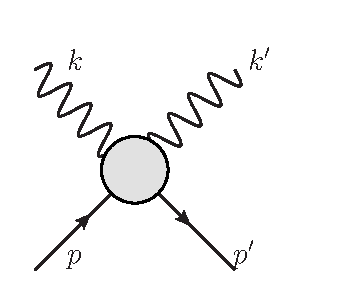
\includegraphics[scale=0.5]{eps/2photon-blob} 
\end{minipage}
$	=	\hspace{1em} 	 $
\begin{minipage}{1.5in}
   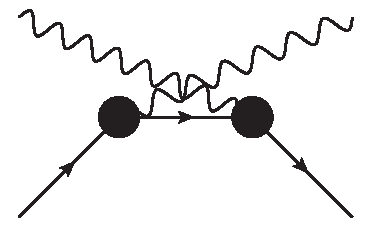
\includegraphics[scale=0.5]{eps/Tree-crossed}
\end{minipage}
$\hspace{1em}   +  \hspace{1em} $
\begin{minipage}{1.5in}
   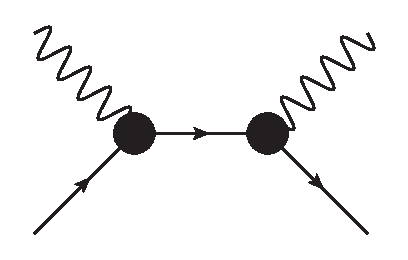
\includegraphics[scale=0.5]{eps/Tree-uncrossed} 
\end{minipage}
} 
\vspace{1em}



While in NRQED, the following diagrams contribute to the scattering:

\vspace{1em}
\begin{minipage}{1in}
   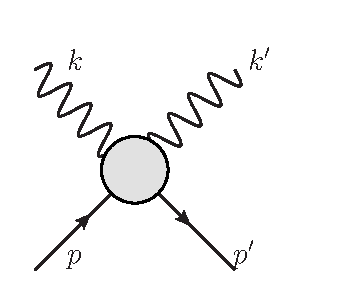
\includegraphics[scale=0.5]{eps/2photon-blob} 
\end{minipage}
$	=	\hspace{1em} 	 $
$\underbrace{ \begin{minipage}{1.3in}
  \begin{center} 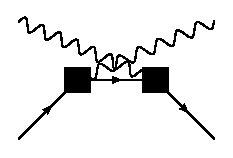
\includegraphics[scale=0.9]{eps/Tree-crossed-square} \end{center}
\end{minipage}}_I$
$\hspace{1em}   +  \hspace{1em} $
$\underbrace{\begin{minipage}{1.3in}
   \begin{center} 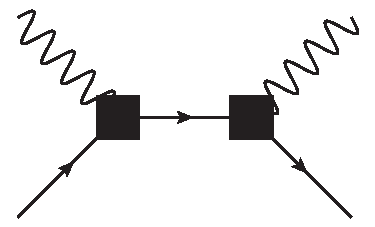
\includegraphics[scale=0.5]{eps/Tree-uncrossed-square} \end{center} 
\end{minipage}}_{II}$
$\hspace{1em}   +  \hspace{1em} $
$\underbrace{\begin{minipage}{1.3in}
   \begin{center} 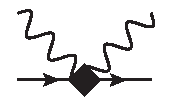
\includegraphics[scale=0.8]{eps/two-photon-nrqed} \end{center} 
\end{minipage}}_{III}$

\vspace{1em}



In each set of diagrams, the vertices represent the \emph{total} electron vertex.  For QED this is determined, as before, by the form factors, and for NRQED it is determined by the calculations of the previous section.

Since the two amplitudes must be equal, in principle the process is this: First calculate the scattering amplitude in QED.  Then, calculate the contribution to the scattering amplitude coming from the tree diagrams I and II above.  Whatever discrepancy remains must be the value of the local two-photon vertex III.   

The process of subtracting the one set of diagrams from the other could be slightly complicated, but luckily it turns out there is a simpler path.  By considering the physical origin of the local terms in NRQED, it will be possible to split the QED diagrams into local and non-local parts, where the latter can be shown to be equal to the non-local diagrams in NRQED.  Then, comparing the two scattering processes becomes much easier.

\subsubsection{Z diagrams}
The high energy theory (QED) doesn't contain any two-photon vertices, while the low energy theory (NRQED) does.  This is a general feature of effective field theories, that new types of local interactions arise.  The high energy theory can have intermediate states that are highly virtual, while the low energy theory doesn't.  Instead, as according to the uncertainty principle, intermediate states with extremely high energy can be considered to occur almost instantaneously, giving rise in the effective theory to local interactions.

How does the local two-photon interaction arise in NRQED?  Of course there are an infinite number of contributions, but we'll consider just the leading order contributions.  These will come from the tree level two photon diagrams as shown above.  Compare the tree-level diagrams in the two theories: in addition to the vertices being different, so are the propagators.  The propagator in QED represents some admixture of the electron and positron field, while in NRQED it is only the electron.
%%%%%%%%
In both QED and NRQED, a process is calculated as the sum of a series of diagrams, representing an expansion in perturbation theory.  However, there is a difference between the two in the nature of perturbation theory employed.

In QED, at each vertex both energy and momentum is conserved.  But intermediate particles may be off mass-shell; that is, it is no longer the case that for a particle of four-momentum $p$ and mass $m$ that $p^2 = m^2$.

In NRQED, the old Rayleigh-Schrodinger perturbation theory is used.   All intermediate particles are on mass-shell.  But at the vertices (when represented diagrammatically), although momenta is conserved, energy is not.  


Remember that in old perturbation theory, corrections have the rough form
\beq
	\Delta =  \Sigma_\text{int} \frac{  \matrixel{\text{out} }{V}{\text{int}} \matrixel{\text{int} }{V}{\text{in}} }{E_\text{in} - E_\text{int}}
	%\Delta = \frac{  \matrixel{A}{B}{C} }{E - E}
\eeq
where the sum is over intermediate states, which can have differing energy from the initial state.

The trick, then, is to take the relativistic tree-level diagrams of QED and rewrite them in the language of  Rayleigh-Schrodinger before trying to compare them to NRQED.  In NRQED, only intermediate states involving electrons can be considered, but in QED intermediate states identified with positrons will appear as well.  It is \emph{these} processes, involving a large violation of energy conservation, that will appear as contact terms in NRQED.  

There are two diagrams in QED, and both can be dealt with in the same general way.  Consider the uncrossed diagram:

%TODO fix diagrams


\vspace{1em}
 \mbox{
\begin{minipage}{1in}
   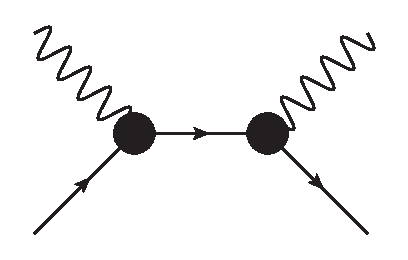
\includegraphics[scale=0.5]{eps/Tree-uncrossed} 
\end{minipage}
$	 \hspace{1em} =	\hspace{1em}	 $
\begin{minipage}{1.5in}
   \begin{center} 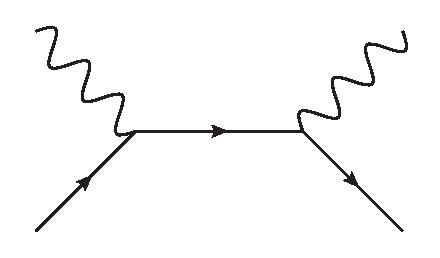
\includegraphics[scale=0.5]{eps/PlainTree} \end{center}
\end{minipage}
$\hspace{1em}   +  \hspace{1em} $
\begin{minipage}{1.5in}
   \begin{center}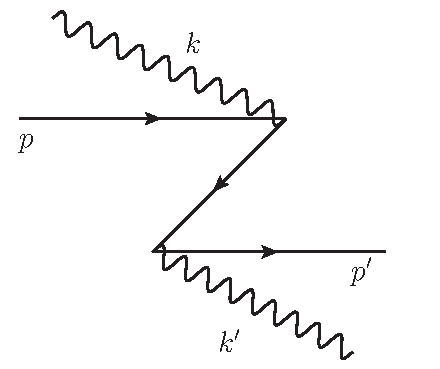
\includegraphics[scale=0.5]{eps/Zdiag} \end{center}
\end{minipage}
} 
\vspace{1em}



There are two tree level processes that can be considered in the old time-ordered perturbation theory.  The first corresponds to an incoming electron, which first absorbs a photon and then emits one.  The second, more complicated process, involves the creation of intermediate positron.  While a free electron travels along, an incoming photon decays into an electron and positron.  Then, the positron annihilates the incoming electron and emits the outgoing photon.  Because of the shape of this diagram, it is called a ``Z diagram.''

In the Z-diagrams, the electrons and the photons are external, so the sum over the intermediate states is specifically the intermediate states of the positrons.  Likewise, the other diagrams are written as a sum over intermediate electron states.  But because of the rules of Rayleigh-Schrodinger perturbation theory, all these states are on mass shell.  And since the momenta here is fixed, the sum over intermediate states is a sum over spin states.

So the original QED diagram should somehow split into two terms, one involving a sum over electron states and the other a sum over anti-particles.  

%TODO insert diagram
Call the intermediate momentum $\v{q}$.  The initial energy will be $q_0$, the intermediate energy will be that of the on mass shell particle, $E_q = \sqrt{\v{q}^2 + m^2 }$.


\vspace{1em}
 \mbox{
\begin{minipage}{1in}
   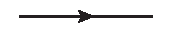
\includegraphics[scale=0.8]{eps/prop} 
\end{minipage}
$	=$ \hspace{1em} $	i\frac{ \cancel{q} -m}{q^2 - m^2}  
		= i\frac{1}{\sqrt{\v{q}^2 + m^2} } \left(
			\frac{ \Sigma u(\v{q}) \bar{u}(\v{q})  }  {q_0 - \sqrt{\v{q}^2 + m^2} }
			+ \frac{ \Sigma v(-\v{q}) \bar{v}(-\v{q})  }  {q_0 + \sqrt{\v{q}^2 + m^2} }
		\right )	 $
} 
\vspace{1em}




This identity can be technically reproduced as follows.  First write the denominator of the propagator as
\beq
	i\frac{ \cancel{q} -m}{q^2 - m^2}   = i \frac{ \cancel{q} -m}{q_0^2 -(\v{q}^2 + m^2)}
\eeq
This could be factored into 
\beq
	q_0^2 -(\v{q}^2 + m^2) = (q_0 + \sqrt{\v{q}^2 + m^2})  (q_0 - \sqrt{\v{q}^2 + m^2})
\eeq
So it implies poles at $q_0 = \pm  \sqrt{\v{q}^2 + m^2}$.  There is one unique way of factoring the original propagator into the two poles:
\beq
	\frac{1}{2\sqrt{\v{q}^2 + m^2}}
		\left(
			\frac{ \gamma^0 \sqrt{\v{q}^2 + m^2} - \v{\gamma} \cdot \v{q} + m}{q_0 - \sqrt{\v{q}^2 + m^2}}
			- \frac{ \gamma^0 \sqrt{\v{q}^2 + m^2} + \v{\gamma} \cdot \v{q} - m}{q_0 + \sqrt{\v{q}^2 + m^2}}
		\right)
\eeq
The two numerators can be exactly equated to sums over polarisation states of electron and positron spinors:
\beqa
	\Sigma u(\v{p}) \bar{u}(\v{p}) &=& \gamma \cdot p + m	\\
	\Sigma v(\v{p}) \bar{v}(\v{p}) &=& \gamma \cdot p - m	
\eeqa
These relations hold for particles which are on mass-shell.  That is exactly the case here.  But then, there is an assumption that the quantity $p_0$ above is the on mass-shell energy, $\sqrt{\v{p}^2 + m^2}$.

So, noting that particles with momentum $\pm \v{q}$ have the same energy $\sqrt{\v{q}^2 + m^2}$ and that $q_0$ is the off-mass shell energy from the relativistic diagram, the propagator can be rewritten:
\beq
	\frac{1}{2\sqrt{\v{q}^2 + m^2}}
		\left(
			\frac{\Sigma u(\v{q}) \bar{u}(\v{q}) }{q_0 - \sqrt{\v{q}^2 + m^2}}
			- \frac{  \Sigma v(-\v{q}) \bar{v}(-\v{q})}{q_0 + \sqrt{\v{q}^2 + m^2}}
		\right)
\eeq
The numerators have now been put into exactly the forms expected for the regular- and Z-diagrams of old perturbation theory. 


As mentioned above this can be understood in the context of old perturbation theory as sum over intermediate states in the numerator,  with the expected form of the denominator being $E_\text{in} - E_\text{int}$.  It can be shown that the denominators have exactly this form. 

Now consider the first, regular diagram.  The initial energy is $q_0$, since in relativistic theory the total energy at the vertex is conserved.  The intermediate energy is the on-mass shell energy of the electron: $\sqrt{\v{q}^2+ m^2}$.  Thus the denominator of $q_0 - \sqrt{\v{q}^2+ m^2}$ is as expected.

Now consider the Z-diagram.  The initial energy is still $q_0$.  The intermediate energy is more complicated: there are two photons, two electrons, and a positron present.  The total combined energy is:
\beq
	E_\text{int} = p_0 + p'_0 + k_0 + k'_0 + \sqrt{\v{q}^2 + m^2} = 2q_0 +  \sqrt{\v{q}^2 + m^2}
\eeq
Then the difference $E_\text{in} - E_\text{int} = -q_0 - \sqrt{\v{q}^2 + m^2}$, as expected.

So rewriting the propagator into these two separate terms can be understood as how the fully relativistic process appears in old perturbation theory.  In a relativistic theory, intermediate states involving positrons must be accounted for.  For higher order QED diagrams more complicated processes will appear, but at the tree level only those discussed above are involved.  No approximations are involved --- the identity for the propagator is exact.  The form is more convenient for discussing nonrelativistic energies, but is still equivalent to the relativistic diagrams.

%Four equations for each of the diagrams





\subsubsection{Relation between NRQED and old perturbation theory}
Now it is necessary to show how the diagrams in old perturbation theory relate to those of NRQED.  

The normal diagrams can be easily interpreted as the product of vertices and the relativistic Rayleigh-Schrodinger propagator:
%Equation with diagram on left, prodcut of verices on right

\vspace{1em}
 \mbox{
\begin{minipage}{1.6in}
   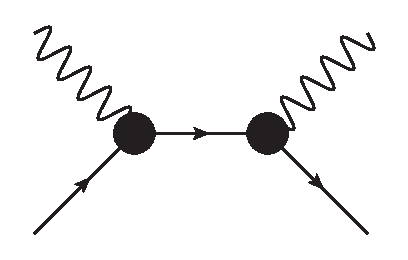
\includegraphics[scale=0.5]{eps/Tree-uncrossed} 
\end{minipage}
$	=	\hspace{2em} 	\Bigg( $
\begin{minipage}{0.8in}
  \begin{center} 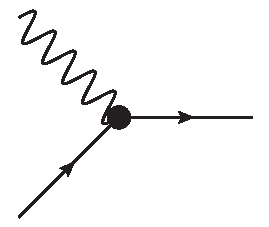
\includegraphics[scale=0.4]{eps/vertex-in} \end{center}
\end{minipage}
$\Bigg ) \times \Bigg ($
\begin{minipage}{0.6in}
   \begin{center} 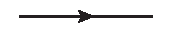
\includegraphics[scale=0.5]{eps/prop} \end{center} 
\end{minipage}
$\Bigg ) \times \Bigg ($\begin{minipage}{0.8in}
   \begin{center} 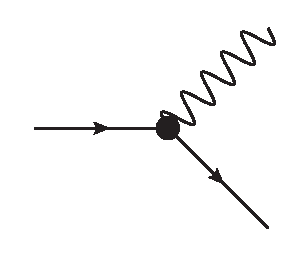
\includegraphics[scale=0.4]{eps/vertex-out} \end{center} 
\end{minipage}
$\Bigg )$
} 
\vspace{1em}
 




%Define each piece
%Vertex in, prop, vertex out
Recall that the total NRQED one-photon vertex was derived by comparing to the QED vertex, so necessarily
\beq
	\bar{u} \Gamma^0 u = \phi^\dagger V^0 \phi , \;  \bar{u} \Gamma^i u = \phi^\dagger V^i \phi
\eeq 
The propagator $1/(q_0 - \sqrt{m^2 + \v{q}^2})$ is equal to the total propagator in NRQED (including relativistic corrections).  So it really is the case that the two sets of diagrams are equivalent.  Whether the vertices are written in terms of NRQED or QED, the ultimate expression will be the same.

It then follows that the contributions to the local contact term in NRQED come (at tree level) exactly from the Z-diagrams.  To calculate the contact terms to the order (in the nonrelativistic expansion) needed, the Z-diagrams need to be approximated just as the one-photon vertex diagrams were in the previous section.  Then the NRQED coefficients can be obtained by comparing the two calculations.  

At nonrelativistic energies, it would be expected that the sum over intermediate states now does not resemble a propagator.  Because only terms involving up to one power of momentum need be kept, the square root term becomes simply $m$.  $q_0$, the total incoming energy, will involve both the electron and photon energy.  Depending on whether the crossed or uncrossed diagram is considered, it will be either $q_0 = p_0 + k_0$ or $q_0 = p_0 - k'_0$.  In either case, it will be $m$ at the leading order, with a first order correction due to the photon energy. 
\beq
	\frac{ \Sigma \bar{v}(-\v{q}) v(-\v{q}) }  {q_0 + \sqrt{\v{q}^2 + m^2} } 
		\approx \frac{ \Sigma \bar{v}(-\v{q}) v(-\v{q}) }  {2m + (q_0-m) }
\eeq
Since $q_0-m << m$, this can then be written as 
\beq
		\approx  \left( 1 - \frac{q_0-m}{2m} \right ) \frac{ \Sigma \bar{v}(-\v{q}) v(-\v{q}) }  {2m}
\eeq
In this approximation, the two Z diagrams become


\vspace{1em}
 \mbox{
\begin{minipage}{1.2in}
   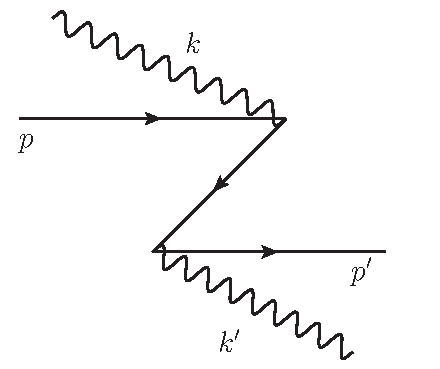
\includegraphics[scale=0.4]{eps/Zdiag} 
\end{minipage}
= \hspace{1em}
\small$	
\Sigma_{\text{spin}}
\left( 1 - \frac{k_0}{2m} \right ) \frac{1}{2m} 
	\bar{u}(\v{p'}) \gamma^\mu \epsilon^*_\mu(k') v_s(-\v{p} - \v{k}) \bar{v}_s(-\v{p} - \v{k}) \Gamma^\nu \epsilon_\nu(k) u(\v{p})
$\normalsize
} 
\vspace{1em}


\vspace{1em}
 \mbox{
\begin{minipage}{1.2in}
   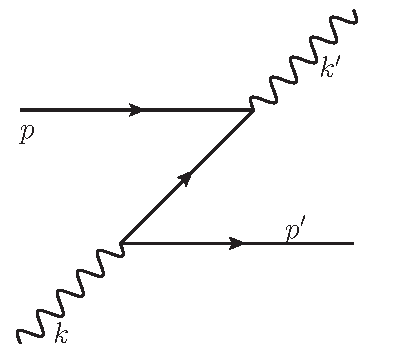
\includegraphics[scale=0.4]{eps/Zdiag2} 
\end{minipage}
= \hspace{1em}
\small $	
\Sigma_{\text{spin}}
\left( 1 + \frac{k'_0}{2m} \right ) \frac{1}{2m} 
	\bar{u}(\v{p'}) \gamma^\mu \epsilon_\mu(k) v(\v{k'} - \v{p})_s \bar{v}_s(\v{k'} - \v{p}) \Gamma^\nu \epsilon^*_\nu(k') u(\v{p})
$ \normalsize
} 
\vspace{1em}

While the sums over intermediate states could also be expanded, it'll be easiest to calculate these in the above form.  The vertices will be the sum of particle-antiparticle bilinears, which can be calculated separately.



\subsection{Nonrelativistic expressions for Z diagrams}


Looking at the equations for the Z diagrams, they are both the product of two types of terms to calculate:

\beq \label{eq:Sh:uvGamma}
	\bar{u}(\v{p'}) \Gamma^\mu(q) v(\gv{\ell}) \;  \text{and} \; \bar{u}(\gv{\ell}) \Gamma^\mu(q) v(\v{p})
\eeq
Here $\ell$ is the intermediate momentum of the positron, and $q$ is the momentum of the photon going into the vertex (either $k$ or $-k'$).  The form of $\Gamma$ is
\beq
	\Gamma^\mu(q) = F_1 \gamma^\mu + F_2 \frac{q_\nu \sigma^{\mu\nu}}{2m}
\eeq
To compare the Z diagrams to the contact terms of NRQED, first express the bilinears in the vertices of \eqref{eq:Sh:uvGamma} in terms of the nonrelativistic quantities.  This can be done for each of the two terms in $\Gamma^\mu$ separately.  The bispinors $u$ will be replaced by the spinor $\phi$, as before.  Now, the bispinor $v$ will be replaced by a spinor for a positron, which shall be called $\chi$.  In doing the expansion only terms up to $\mathcal{O}(1/m)$ need be kept.


To calculate the vector like bilinears, treat the spatial and time-like components separately.  First $\mu=0$:
\beqa
	\ubar(p') \gamma^0 v(\ell)
		&=&	\udaggervec{\v{p'}} \vvec{\v{q}}	\\
		&=&	\phi^\dagger \left( \frac{ \sigdot{\ell} + \sigdot{p'} }{2m} \right ) \chi	\\
	\vbar{\ell} \gamma^0 u(p)
		&=&	\vdaggervec{\ell} \uvec{p}	\\
		&=&	\chi^\dagger \left( \frac{ \sigdot{\ell} + \sigdot{p} }{2m} \right ) \phi	
\eeqa
Then $\mu=i$:
\beqa
	\ubar(p') \gamma^i v(\ell)
		&=&	\udaggervec{p'} \begin{pmatrix} 0 & \sigma_i \\ \sigma_i & 0 \end{pmatrix} \vvec{\ell}	\\
		&=&	\phi^\dagger \sigma_i \chi \\
	\vbar(\ell) \gamma^i u(p)
		&=&	\vdaggervec{\ell} \begin{pmatrix} 0 & \sigma_i \\ \sigma_i & 0 \end{pmatrix} \uvec{p}	\\
		&=&	\chi^\dagger \sigma_i \phi 
\eeqa

In the tensor terms a factor of momentum $q_\nu$ appears.  The spatial part, $q_j$ is ``naturally raised" so $q_j = -(\v{q})_j$.  As before the two types of indices should be treated separately.  For $\mu=0$:

\beqa
	\frac{i q_\nu}{2m} \ubar(p') \sigma^{0 \nu} v(\ell) 
		&=& \frac{i q_j}{2m} \ubar(p') \sigma^{0j} v(\ell) \\
		&=& -\frac{q_j}{2m} \udaggervec{p'} \Mblock{0}{\sigma^i}{-\sigma^i}{0} \vvec{\ell}	\\
		&=& \phi^\dagger \frac{ \sigdot{q}}{2m} \chi	\\
	\frac{i q_\nu}{2m} \vbar(\ell) \sigma^{0 \nu} u(p) 
		&=& \frac{i q_j}{2m} \vbar(\ell) \sigma^{0j} u(p) \\
		&=& -\frac{q_j}{2m} \vbar{\ell} \Mblock{0}{\sigma^i}{-\sigma^i}{0} \uvec{p}	\\
		&=& -\chi^\dagger \frac{ \sigdot{q}}{2m} \phi	\\
\eeqa
Then for $\mu=i$
\beq
	\frac{i q_\nu}{2m} \ubar(p') \sigma^{i \nu} v(\ell)
	 	= \frac{i q_0}{2m} \ubar(p') \sigma^{i 0} v(\ell) + \frac{i q_j}{2m} \ubar(p') \sigma^{i j} v(\ell)	
\eeq
\beq
	 = - \frac{i q_0}{2m}  \udaggervec{p'} \Mblock{0}{\sigma^i}{-\sigma^i}{0} \vvec{\ell} 	
	 	+ \frac{i q_j}{2m}  \epsilon_{ijk}  \udaggervec{p'} \Mblock{\sigma^k}{0}{0}{\sigma^k} \vvec{\ell} \nonumber
\eeq
The second term will be of order $\mathcal{O}(1/m^2)$ and so can be neglected.  So 
\beq
	\frac{i q_\nu}{2m} \ubar(p') \sigma^{i \nu} v(\ell) 
		= \phi^\dagger \frac{q_0 \sigma_i}{2m} \chi
\eeq
The complementary term is 
\beq
	\frac{i q_\nu}{2m} \vbar(\ell) \sigma^{i \nu} u(p)
	 	= \frac{i q_0}{2m} \vbar(\ell) \sigma^{i 0} v(\ell) + \frac{i q_j}{2m} \ubar(p') \sigma^{i j} u(p)	
\eeq
Again,  the second term with $\sigma^{ij}$ has the same general structure and will be of order $1/m^2$.  So 
\beqa
		\frac{i q_\nu}{2m} \vbar(\ell) \sigma^{i \nu} u(p)
	 &=&	\frac{i q_0}{2m} \vdaggervec{\ell} \Mblock{0}{\sigma^i}{-\sigma^i}{0} \uvec{p} 	\\
	 &=&	- \chi^\dagger \frac{q _0 \sigma^i}{2m} \phi
\eeqa

Now the total vertices $\ubar \Gamma^\mu v$ can be expressed nonrelativistically:

\beq
	\ubar(p') \Gamma^0 v(\ell)  
		=  \phi^\dagger(p') \left( F_1 \frac{ \sigdotg{\ell} + \sigdot{p'} }{2m} + F_2 \frac{ \sigdot{q} } {2m} \right ) \chi(\ell)
\eeq

\beq
	\vbar(\ell) \Gamma^0 v(p)  
		=  \chi^\dagger(p') \left( F_1 \frac{ \sigdotg{\ell} + \sigdot{p} }{2m} + F_2 \frac{ \sigdot{q} } {2m} \right ) \phi(\ell)
\eeq
	
\beq
	\ubar(p') \Gamma^i v(\ell)  
		= \phi^\dagger \left( F_1 + F_2 \frac{q_0}{2m} \right) \sigma^i \chi
\eeq
			
\beq
	\vbar(\ell) \Gamma^i v(p)  
		= \chi^\dagger \left( F_1 - F_2 \frac{q_0}{2m} \right) \sigma^i \phi
\eeq			

Returning to the Z diagrams, the structures $\Gamma^\mu$ appear contracted with the photon polarization.  Because a physical process is being calculated, the result should not depend on the gauge chosen.  So it will be easiest to choose the gauge where the photons are transverse and $\epsilon_0 = 0$.  Then $\Gamma \cdot \epsilon = - \gv{\Gamma} \cdot \gv{\epsilon}$.

\vspace{1em}
 \mbox{
\begin{minipage}{1in}
   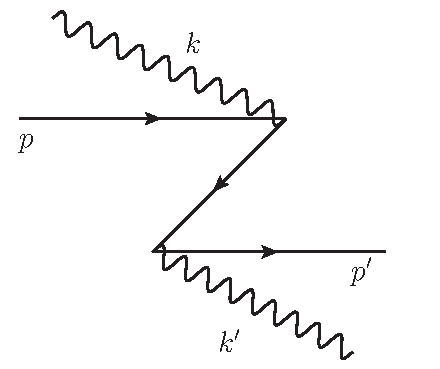
\includegraphics[scale=0.4]{eps/Zdiag} 
\end{minipage}
 = \hspace{0.5em}
\begin{minipage}{3in}
\beq
\begin{split}
	\Sigma_{\text{spin}}
	\left( 1 - \frac{k_0}{2m} \right ) &\frac{1}{2m} 
		\left[ \phi^\dagger \left( F_1 + F_2 \frac{ -k'_0}{2m} \right ) \gv{\sigma} \cdot \gv{\epsilon}^*(k') \chi \right]
\\ &	\times	\left[ \epsilon_j(k) \chi^\dagger \left( F_1 - F_2 \frac{k_0}{2m} \right)  \gv{\sigma} \cdot  \gv{\epsilon}(k)   \phi \right ]	
\end{split}
\eeq
\end{minipage}
} 
\vspace{1em}

The sum over intermediate spin spates just becomes the identity: $\Sigma_{\text{spin}} \chi^\dagger \chi = 1$. 
\beq
	= \frac{1}{2m} \left( 1 - \frac{k_0}{2m} \right ) \phi^\dagger \left[ 
			\left( F_1 - F_2 \frac{k'_0}{2m} \right )
			\left( F_1 - F_2 \frac{k_0}{2m} \right)
			\gv{\sigma} \cdot \gv{\epsilon}^*(k')  \gv{\sigma} \cdot  \gv{\epsilon}(k)  
		\right ] \phi
\eeq
	
Since only terms up to order $1/m$ are needed, this can be simplified.  Also, in this approximation $k'_0 \approx k_0$, as the total conservation of energy implies $k'_0 - k_0 = p_0 - p'_0 \sim \v{p}^2/m^2$.  So for convenience everything will be written in terms of $k_0$.  

\beq
	= \frac{1}{2m}  \phi^\dagger \left[ 
			\left( F_1^2 - F_1 [F_1 + 2 F_2 ] \frac{k_0}{2m} \right )
			\gv{\sigma} \cdot \gv{\epsilon}^*(k')  \gv{\sigma} \cdot  \gv{\epsilon}(k)  
		\right ] \phi
\eeq


The other Z diagram, coming from the crossed diagram is:

\vspace{1em}
 \mbox{
\begin{minipage}{1in}
   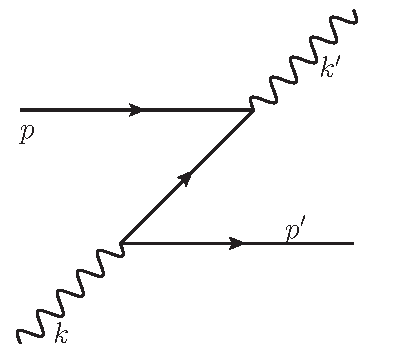
\includegraphics[scale=0.4]{eps/Zdiag2} 
\end{minipage}
= \hspace{0.5em}
\scriptsize$	
\Sigma_{\text{spin}}
\left( 1 + \frac{k'_0}{2m} \right ) \frac{1}{2m} 
	\left[ \phi^\dagger \left( F_1 + F_2 \frac{ k_0}{2m} \right ) \gv{\sigma} \cdot \gv{\epsilon}^(k) \chi \right]
	\left[ \epsilon_j(k) \chi^\dagger \left( F_1 + F_2 \frac{k'_0}{2m} \right)  \gv{\sigma} \cdot  \gv{\epsilon}^*(k')   \phi \right ]	
$\normalsize
} 
\vspace{1em}

After summing over spin states this becomes
\beq
	 \frac{1}{2m} \left( 1 + \frac{k'_0}{2m} \right ) \phi^\dagger \left[ 
			\left( F_1 + F_2 \frac{k_0}{2m} \right )
			\left( F_1 + F_2 \frac{k'_0}{2m} \right)
			\gv{\sigma} \cdot \gv{\epsilon}^(k)  \gv{\sigma} \cdot  \gv{\epsilon}^*(k')  
		\right ] \phi.
\eeq
And then applying the same simplifications as before results in
\beq
	 \frac{1}{2m}  \phi^\dagger \left[ 
			\left( F_1^2 + F_1 [F_1 + 2 F_2 ] \frac{k_0}{2m} \right )
			\gv{\sigma} \cdot \gv{\epsilon}^(k)  \gv{\sigma} \cdot  \gv{\epsilon}^*(k')  
		\right ] \phi.
\eeq

The local interaction comes from the sum of the two diagrams.  Adding them together,

%TODO add diagram?
\mbox{
\begin{minipage}{0.6in}
   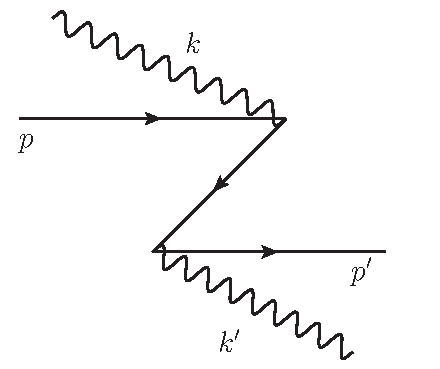
\includegraphics[scale=0.2]{eps/Zdiag} 
\end{minipage}
+
\begin{minipage}{0.6in}
   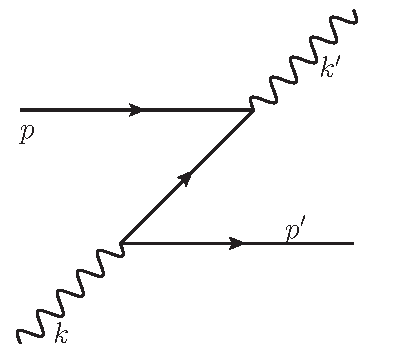
\includegraphics[scale=0.2]{eps/Zdiag2} 
\end{minipage}
\begin{minipage}{2in}
\begin{equation*}
=
\begin{split}
 & \frac{1}{2m} \phi^\dagger \Bigg [
	 \left( F_1^2 + F_1 [F_1 + 2 F_2 ] \frac{k_0}{2m} \right )
			\gv{\sigma} \cdot \gv{\epsilon}^(k)  \gv{\sigma} \cdot  \gv{\epsilon}^*(k')  \\
	&+ 
			\left( F_1^2 - F_1 [F_1 + 2 F_2 ] \frac{k_0}{2m} \right )
			\gv{\sigma} \cdot \gv{\epsilon}^*(k')  \gv{\sigma} \cdot  \gv{\epsilon}(k)  
		 \Bigg ] \phi	
\end{split}
\end{equation*}
\end{minipage}
}
\beq
\begin{split}
=&
		\frac{F_1}{2m}  \phi^\dagger \Bigg [
			F_1 \{ \gv{\sigma} \cdot \gv{\epsilon},   \gv{\sigma} \cdot  \gv{\epsilon}^* \}
			+ (F_1 + 2F_2) \frac{k_0}{2m} [ \gv{\sigma} \cdot \gv{\epsilon},   \gv{\sigma} \cdot  \gv{\epsilon}^* ]
		 \Bigg ] \phi	\\
	=&
		\frac{F_1}{m}  \phi^\dagger \Bigg [
			F_1  \gv{\epsilon} \cdot  \gv{\epsilon}^* 
			+ (F_1 + 2F_2) \frac{k_0}{2m} \gv{\sigma} \cdot \gv{\epsilon} \times  \gv{\epsilon}^* 
		 \Bigg ] \phi
\end{split}
\eeq
It now remains to calculate the same amplitude in NRQED and compare.
		
\subsection{Compton scattering in NRQED}
The idea is to calculate the Compton scattering in the nonrelativistic theory.  The gauge is chosen such that the photon polarisations obey $\epsilon_0 = 0$.  In general, both terms arising from two-photon vertices, and those from tree level diagrams of two one-photon vertices, should be considered.  However, because of the approach taken in calculating the process from the relativistic Lagrangian, only the former terms are needed.  That is, contact terms (which arise from some combination of Z-diagrams in the relativistic theory)  are separated from the rest.  

Further, ultimately only a few of these terms are relevant -- terms which have both $\v{B}$ and $\v{A}$ can be ignored.

The remaining terms of interest are:
\scriptsize
\beqa
	\mathcal{L}_{A^2} &=& \fnr^\dagger ( - \frac{e^2 \v{A}^2}{2m}  - e^2 \frac{ \{ \grad^2, \v{A}^2 \} 
}{8m^3} - e^2\frac{ \{\nabla_i, A_i \} \{\nabla_j, A_j\} }{8m^3}
		+ c^2_S \frac{ e^2 \v{S} \smalldot ( \v{A} \times \v{E} - \v{E} \times \v{A} )}{8m^2} ) \fnr
\eeqa
\normalsize

The process considered has an incoming photon with momentum $k$ and polarisation $\epsilon(k)$, and an outgoing photon with momentum $k'$ and polarisation $\epsilon^*(k')$.  The charged particle has incoming momentum $p$ and outgoing $p'= p + k - k'$.

As in the single-photon calculation, it is simply a matter of reading terms off the Lagrangian.  To find the scattering amplitude,  replace $\Psi$ with $\phis$, and replace $\v{A}$ with photon polarisations $\epsilon$ and $\epsilon^*$.  In the gauge chosen, $\v{E}(k) = -\partial_0 \v{\A} = i k_0 \gv{\epsilon}(k) = -ik'_0 \gv{\epsilon^*}(k') $ .

Contracted with the photon of momentum $k$, the result is $\v{E} \to i k_0 \v{\A}$, while with the photon of momentum $k'$ it is $\v{E} \to i k'_0 \v{\Adag}$.  Both processes must be considered in calculating the scattering, so:
\[
	\v{A} \times \v{E} = - \v{A} \times (\partial_0 \v{A})
		\to 
	-i(k_0' \v{\epsilon} \times \v{\epsilon} - k_0 \v{\epsilon} \times \v{\epsilon} ) = i ( k_0' + k_0) \v{\epsilon} \times \v{\epsilon}^*
\]
And
\[
	\v{E} \times \v{A} = - (\partial_0 \v{A}) \times  \v{A}
		\to 
	-i( k_0 \v{\epsilon} \times \v{\epsilon^*} - k_0' \v{\epsilon^*} \times \v{\epsilon} ) = -i ( k_0' + k_0) \v{\epsilon} \times \v{\epsilon^*}
\]
So from the term in the Lagrangian 
\[
 c_S \Psi^\dagger \frac{ e^2 \v{S} \smalldot ( \v{A} \times \v{E} - \v{E} \times \v{A} )}{8m^2} ) \Psi
\]
appears in the scattering amplitude
\[
  -i c_S \phi^\dagger  \Big ( \frac{e^2}{4m^2}    i(k_0 + k_0')    \v{\epsilon} \times \v{\epsilon^*} \Big ) \phi
	=
     c_S \frac{e^2}{4m^2} \phi^\dagger  \Big ( (k_0 + k_0')    \v{\epsilon} \times \v{\epsilon^*} \Big ) \phi
\]
Using the approximation $k_0 \approx k'_0$, that part of the amplitude now becomes
\beq \label{eq:Sh:ComptNR}
     c_S \frac{e^2}{2m^2} \phi^\dagger  \Big ( k_0    \v{\epsilon} \times \v{\epsilon^*} \Big ) \phi
\eeq


This is the part of the amplitude wanted to compare for reasons of consistency.
	

\subsection{Comparison of QED and NRQED Compton scattering}
Now that the amplitude has been calculated in both theories, the coefficient of NRQED $c_S$ can be fixed.  Using that $F_1 = e$ and $F_2 = e\frac{g-2}{2}$, $F_1 + 2F_2 = e^2(g-1)$.
So the final result is that 
\beq
	c_S = g-1
\eeq
 






\chapter{General Spin Formalism}

%name? 

Our ultimate goal is to calculate corrections to the $g$-factor of a loosely bound charged particle of arbitrary spin.  Our strategy is to obtain an effective Lagrangian in the nonrelativistic limit.

We first consider features of a general-spin formalism in both the relativistic and nonrelativistic cases, and the connection between the wave functions of the free particles.  Then we consider how constraints of the relativistic theory let us calculate scattering off an external field.  Comparing this result to that done with an effective NRQED Lagrangian, we can obtain the coefficients of that Lagrangian for particles of general spin.




\subsection{Spinors for general-spin charged particles}


\subsubsection{Relativistic bispinors}
First we need to work out a formalism that will apply to the general spin case.  
We want to represent the spin state of the particles by an object that looks like a generalization of the Dirac bispinor.

%TODO check what to call helical basis
It is easiest to start with the Dirac basis, where the upper and lower components of the bispinor are objects of opposite helicity, each transforming as an object of spin $1/2$.

To that end define an object

\beq \label{eq:PsiDef}
\Psi  = \frac{1}{\sqrt{2}} \begin{pmatrix} \xi \\ \eta \end{pmatrix}
\eeq

that we wish to have the appropriate properties.  Each component should transform as a particle of spin $s$, but with opposite helicity.  Under reflection the upper and lower components transform into each other.

Representations of the proper Lorentz group are spinors which are separately symmetric in dotted and undotted indices.  If $\xi$ is an object with $p$ undotted and $q$ dotted indices
\beq
	\xi = \{ \xi^{\alpha_1 \ldots \alpha_p}_{\dot\beta_1 \ldots \dot\beta_q} \}
\eeq
Then this can be a representation of a particle of spin $s = (p+q)/2$.

We have some free choice in how to partition the dotted/undotted indices, and we cannot choose exactly the same scheme for all spin as long as both types of indices are present.  However, we can make separately consistent choices for integral and half-integral spin.  For integral spin we can say $p=q=s$, while for the half-integral case we'll choose $p=s+\frac{1}{2}$, $q=s-\frac{1}{2}$.

We want the $\xi$ and $\eta$ to transform as objects of opposite helicity.  Under reflection they will transform into each other.  So 
\beq
	\eta = \{ \eta_{\dot \alpha_1 \ldots \dot \alpha_p}^{\beta_1 \ldots \beta_q} \}
\eeq




In the rest frame of the particle, they will have clearly defined and identical properties under rotation.    The rest frame spinors are equivalent to rank $2s$ nonrelativistic spinors.  So the bispinor in the rest frame looks like
\beq \label{eq:PsiRest}
\Psi = \frac{1}{\sqrt{2}} \begin{pmatrix} \xi_0 \\ \xi_0 \end{pmatrix}
\eeq

where
\beq \label{eq:xi0def}
	\xi_0 = \{ (\xi_0)_{\alpha_1 \ldots \alpha_p \beta_1 \ldots \beta_q}  \}
\eeq
and all indices are symmetric.

We can obtain the spinors in an arbitrary frame by boosting from the rest frame.  The upper and lower components we have defined to have opposite helicity, and so will act in opposite ways under boost:
\beq \label{eq:xi0boosted}
	\xi = \exp{(\frac{\v{\Sigma} \cdot \v{\rapidity}}{2}) } \xi_0,  
	\hspace{3em} 
	\eta = \exp{(-\frac{\v{\Sigma} \cdot \v{\rapidity}}{2}) } \xi_0
\eeq

%TODO check dotted/undotted transformations are correct
What form should the operator $\v{\Sigma}$ have?  Under an infinitesimal boost by a rapidity $\phi$, a spinor with a single undotted index is transformed as
\beqB
	\xi_\alpha \to \xi'_\alpha = \left(\delta_{\alpha \beta} + \frac{\gv{\rapidity}\cdot \gv{\sigma}_{\alpha \beta} }{2} \right) \xi_\beta 
\eeqB
while one with a dotted index will transform as
\beqB
\xi_{\dot\alpha} \to \xi'_{\dot\alpha} = \left(\delta_{\dot \alpha \dot \beta} - \frac{\gv{\rapidity}\cdot \gv{\sigma}_{\dot \alpha \dot\beta} }{2} \right) \xi_{\dot \beta}
\eeqB



The infinitesimal transformation of a higher spin object with the first $p$ indices undotted and the last $q$ dotted would then be
\beqB
	\xi \to \xi' = \left(1 
		+  \sum\limits_{a=0}^p \frac{\gv{\sigma}_a \cdot \gv{\rapidity} }{2}
		- \sum\limits_{a=p+1}^{p+q} \frac{\gv{\sigma}_a \cdot \gv{\rapidity} }{2}
	\right ) \xi 
\eeqB
where $a$ denotes which spinor index of $\xi$ is operated on.


If we define 
\beq \label{eq:SigDef}
	\v{\Sigma} = \sum\limits_{a=0}^p \gv{\sigma}_a - \sum\limits_{a=p+1}^{p+q} \gv{\sigma}_a 
\eeq

Then the infinitesimal transformations would be
\beqB
	\xi \to \xi' = \left( 1 + \frac{\gv{\Sigma} \cdot \gv{\rapidity} }{2} \right) \xi
\eeqB
\beqB
	\eta \to \eta' = \left( 1 - \frac{\gv{\Sigma} \cdot \gv{\rapidity} }{2} \right) \eta
\eeqB
So the exact transformation should be
\beqB
		\xi \to \xi' = \exp\left( \frac{\gv{\Sigma} \cdot \gv{\rapidity} }{2} \right) \xi
\eeqB
\beqB
	\eta \to \eta' = \exp \left( -\frac{\gv{\Sigma} \cdot \gv{\rapidity} }{2} \right) \eta
\eeqB
  
Therefore, the bispinor of some particle boosted by $\gv{\phi}$ from rest will be
% TODO check passive v. active boost
\beq \label{eq:PsiByXi0}
\Psi = \frac{1}{\sqrt{2}} \begin{pmatrix} 
		\exp\left( \frac{\gv{\Sigma} \cdot \gv{\rapidity} }{2} \right)\xi_0 \\ 
		\exp \left( \frac{-\gv{\Sigma} \cdot \gv{\rapidity} }{2} \right) \xi_0 
	\end{pmatrix}
\eeq

%TODO fix sqrt(2) factors in the right place
In dealing with the relativistic theory, we'll want a basis that separates the particle and antiparticle parts of the wave function.  If we want the upper component to be the particle, then in the rest frame the lower component will vanish, and for low momentum will be small compared to the upper component.  The unitary transformation which accomplishes this is

\[
	\Psi' = \begin{pmatrix} \phi \\ \chi \end{pmatrix}
\]

\[
	\phi = \frac{1}{\sqrt{2}}(\xi + \eta)
\]
\[
	\chi = \frac{1}{\sqrt{2}}( \eta - \xi)
\]


Which is equivalent to
\[
	\Psi' = \frac{1}{\sqrt{2}} \begin{pmatrix}1 & 1 \\ -1 & 1 \end{pmatrix} \Psi
\]

Then,
\beq \label{eq:phiDef}
	\phi =  \cosh \left( \frac{\gv{\Sigma} \cdot \gv{\rapidity} }{2} \right ) \xi_0
\eeq

%Sign confusion compared to original equation again
\beq \label{eq:chiDef}
	\chi =  \sinh \left( \frac{\gv{\Sigma} \cdot \gv{\rapidity} }{2} \right ) \xi_0
\eeq

\subsubsection{Spinors for nonrelativistic theory}

We also need to discuss the nonrelativistic, single-particle theory.  This is much simpler: the spin state of particles in this theory is represented by symmetric spinors with $2s+1$ undotted indices.  The only operators we need to consider acting on this space are spin matrices and products of spin matrices. 

%Section on bilinear transforms
%
%FIXME check for possible typos in calculations (I seem to remember there were some here?)


\section{Transformations of bilinears in the case of general spin}
\label{chap:bilinear}
We have the transformation of the spinor under small boosts:
\beqa
	\Psi &\to& \Psi' = \Psi + \frac{\eta_i }{2} \begin{pmatrix} 0 & \Sigma_i \\ \Sigma_i & 0 \end{pmatrix}\Psi
\eeqa
\beqa
	\bar{\Psi} &\to& \bar{\Psi'} = \bar{\Psi} - \frac{\eta_i }{2} \bar{\Psi} \begin{pmatrix} 0 & \Sigma_i \\ \Sigma_i & 0 \end{pmatrix}
\eeqa

We can also see the transformation of the spinor under parity: simply put, because the upper component is even in $\gv{\Sigma} \cdot \v{p}$, whereas the lower component is odd, we obtain
\[
	\Psi \to \begin{pmatrix} 1 & 0 \\ 0 & -1 \end{pmatrix}\Psi
\]
\[	\bar{\Psi} \to \bar{\Psi} \begin{pmatrix} 1 & 0 \\ 0 & -1 \end{pmatrix}
\]
So
\[
	\bar{\Psi} \begin{pmatrix} A & B \\ C & D \end{pmatrix} \Psi
		\to
	\bar{\Psi} \begin{pmatrix} A & -B \\ -C & D \end{pmatrix} \Psi
\]

From these facts we can examine the general behavior of bilinears under Lorentz transformations.

Now we'll examine the behavior of bilinears under boosts.  We can write the general structure of the bilinear as
\[
	\bar{\Psi} T \Psi = 	\bar{\Psi} \begin{pmatrix} A + D & B+C \\ B-C & A - D \end{pmatrix} \Psi
\]
or using a different notation
\[
\bar{\Psi} T \Psi = 	\bar{\Psi} 
	\left [
			A \otimes \begin{pmatrix} 1 & 0 \\ 0 & 1 \end{pmatrix}
			+ D \otimes \begin{pmatrix} 1 & 0 \\ 0 & -1\end{pmatrix}			
			+ B \otimes \begin{pmatrix} 0 & 1 \\ 1 & 0 \end{pmatrix}
			+ C \otimes \begin{pmatrix} 0 & 1 \\ -1 & 0 \end{pmatrix}
	\right)]  \Psi
\]

Under an infitesimal Lorentz boost $\gv{\eta}$ this will transform into
\[
	\bar{\Psi} T \Psi \to \bar{\Psi} T \Psi
		+ \frac{\eta_i}{2} \bar{\Psi} \left (  \begin{pmatrix} A + D & B+C \\ B-C & A - D \end{pmatrix} \begin{pmatrix} 0 & \Sigma_i \\ \Sigma_i & 0 \end{pmatrix} - \begin{pmatrix} 0 & \Sigma_i \\ \Sigma_i & 0 \end{pmatrix} \begin{pmatrix} A + D & B+C \\ B-C & A - D \end{pmatrix} \right ) \Psi					
\]
We can express this in terms of commutators and anti-commutators
\[
	\bar{\Psi} T \Psi \to \bar{\Psi} T \Psi
		+ \frac{\eta_i}{2} \bar{\Psi} \left [
			[B, \Sigma_i] \otimes \begin{pmatrix} 1 & 0 \\ 0 & 1 \end{pmatrix}
			+ [A, \Sigma_i] \otimes \begin{pmatrix} 0 & 1 \\ 1 & 0 \end{pmatrix}
 			+ \{C, \Sigma_i\} \otimes \begin{pmatrix} 1 & 0 \\ 0 & -1\end{pmatrix}
			+ \{D, \Sigma_i\} \otimes \begin{pmatrix} 0 & 1 \\ -1 & 0 \end{pmatrix}
	\right)] \Psi
\]

We can note here that, using only the matrices $\gv{\Sigma}$ and $\gv{S}$ we can build three structures invariant under rotations: and $S^2$, $\Sigma^2$, and $\Sigma \cdot S$.  All three of these structures commute with both $S_i$ and $\Sigma_i$, and their value depends only on the particular representation we're working with.  So for our purposes here, they can just be treated as pure numbers.


\subsubsection{Scalar bilinears}
Since the scalar must be invariant to rotation, then by the logic above it's block elements are proportional to the identity.

It must also be unchanged under boosts.  We can see that this necessitates that $C=D=0$, while providing no constraint on A and B.  So the general form of a bilinear invariant under boosts is
\[
	\bar{\Psi} T \Psi = \bar{\Psi} \begin{pmatrix} A & B \\B & A \end{pmatrix} \Psi
\]
where A and B are proportional to the identity.

Under the discrete partiy transformation this will transform into
\[
	\bar{\Psi} T' \Psi = \bar{\Psi} \begin{pmatrix} A & -B \\-B & A \end{pmatrix} \Psi
\]
This shows that for a true scalar, $B=0$.


\subsubsection{Vector bilinears}
To attempt to construct a vector bilinear, we can start by considering the time-like part of it.  Since this must be invariant under spatial rotations, then by the same logic as above it must essentially be composed of four blocks proportional to the identity.  We also know that under boosts the time-like part is transformed into the spatial and vice versa, so we can use these linked transformations to obtain constraints on the bilinear.

If $T^\mu$ is a vector we know that, under an infinitesimal boost, it's transformation will be
\beqa
	T^0 &\to& T^0 + \eta_i T^i	\\
	T^i &\to& T^i + \eta_i T^0
\eeqa

We again write 
\[T^\mu = \begin{pmatrix}A^\mu + D^\mu & B^\mu+C^\mu \\ B^\mu-C^\mu & A^\mu - D^\mu  \end{pmatrix} \]

Then we see that under boost, $T^0$ transforms as

\[
	\bar{\Psi} T^0 \Psi \to 	\bar{\Psi} T^0 \Psi
	+  \eta_i \bar{\Psi} \left [
			C^0 \Sigma_i \otimes \begin{pmatrix} 1 & 0 \\ 0 & -1\end{pmatrix}
			+ D^0 \Sigma_i \otimes \begin{pmatrix} 0 & 1 \\ -1 & 0 \end{pmatrix}
	\right] \Psi
\]
where we've used that fact that all the components of $T^0$ commute with $\Sigma_i$.
This tells us that for $T^\mu$ to be a 4-vector, the following must be true.
\beqa
	A^i &=& 0	\\
	B^i &=& 0 	\\
	C^i &=& D^0 \Sigma^i	\\
	D^i &=& C^0 \Sigma^i	\\
\eeqa

We can now consider how $T^i$ changes under a boost, and discover

\beqa
\bar{\Psi} T^i \Psi 
	&\to& \bar{\Psi} T^i \Psi
		+ \frac{\eta_j}{2} \bar{\Psi} \left [
			\{C^i, \Sigma^j\} \otimes \begin{pmatrix} 1 & 0 \\ 0 & -1\end{pmatrix}
			+ \{D^i, \Sigma^j\} \otimes \begin{pmatrix} 0 & 1 \\ -1 & 0 \end{pmatrix}
		\right)] \Psi	\\
	&=& \bar{\Psi} T^i \Psi
		+ \frac{\eta_j}{2} \bar{\Psi} \left [
			D^0\{\Sigma^i, \Sigma^j\} \otimes \begin{pmatrix} 1 & 0 \\ 0 & -1\end{pmatrix}
			+ C^0\{\Sigma^i, \Sigma^j\} \otimes \begin{pmatrix} 0 & 1 \\ -1 & 0 \end{pmatrix}
		\right)] \Psi	\\
\eeqa
Again considering our demand that $T^\mu$ transform like a 4-vector, we get
\beqa
	A^0 &=& 0	\\
	B^0 &=& 0	\\
	C^0 \delta^{ij} &=&  C^0 \frac{1}{2}\{\Sigma^i, \Sigma^j\}	\\
	D^0 \delta^{ij} &=&  D^0 \frac{1}{2}\{\Sigma^i, \Sigma^j\}	\\
\eeqa
The last two constraints are met in the spin-1/2 case, but not for higher spins.  This tells us that there's no way to, in the higher spin case, construct a vector bilinear using only I, $\gv{\Sigma}$, and $\v{S}$.

For spin-1/2, where $\Sigma_i = \sigma_i$, we see that a true vector bilinear (with correct transformation properties under parity) will be proportional to 
\[
	(T^0, \v{T} ) = \left( \begin{pmatrix} 1 & 0 \\ 0 & -1 \end{pmatrix} , \begin{pmatrix} 0 & \gv{\sigma} \\ -\gv{\sigma} & 0 \end{pmatrix} \right )
\]
which, of course, is exactly what we knew already.

\subsubsection{Tensor bilinears}
Here we'll be a little less ambitious.  We can tell from the above considerations that, under boosts, we effectively mix A and B components seperately from the C and D blocks.  What's more, we need anti-commutation relationships to deal with the latter transformations.  So we'll just consider tensors that look like
\[
	T^{\mu\nu} = \begin{pmatrix} A^{\mu\nu} & B^{\mu\nu} \\ B^{\mu\nu} & A^{\mu\nu} \end{pmatrix}	
\]
Furthermore, we'll consider only anti-symmetric tensors for now.  Now we can basically procede as in the vector case, knowing how an anti-symmetric tensor should transform:
\beqa
	T^{0i} &\to& T^{0i} +  \eta_j T^{ji}	\\
	T^{ij}	&\to& T^{ij} + \eta_i T^{0j} + \eta_j T^{i0}	\\
\eeqa

Start by considering the components of $T^{0i} = -T{i0}$.  They must transform as vectors under rotations.  We have two vectors available to us, so we can write
\beqa
	A^{0i} &=& \alpha \Sigma^i + \beta S^i	\\
	B^{0i} &=& \gamma \Sigma^i + \delta S^i	\\
\eeqa

Under a boost, we find the relation that
\beqa
	A^{ji} &=& [B^{0i}, \Sigma^j]	\\
	B^{ji} &=& [A^{0i}, \Sigma^j]	\\	
\eeqa
And then looking at how $T^{ij}$ transforms, we get the constraint
\beqa
	\eta_k \left[ [A^{0i}, \Sigma^j], \Sigma^k \right] &=& \eta_j A^{0i} - \eta_i A^{0j}	\\
	\eta_k \left[ [B^{0i}, \Sigma^j], \Sigma^k \right] &=& \eta_j B^{0i} - \eta_i B^{0j}	\\
\eeqa
We're assuming that both $A^{0i}$ and $B^{0i}$ are linear combinations of $\Sigma_i$ and $S_i$.  So what we need are the relationships
\beqa
	[\Sigma^i, \Sigma^j] &=& 4 i \epsilon_{ijk} S^k	\\
	{}[S^i, \Sigma^j] &=& i\epsilon_{ijk} \Sigma^k 	\\
	{}[[\Sigma^i, \Sigma^j], \Sigma^k] 
		&=& 4 i\epsilon_{ij\ell} [S^\ell, \Sigma^k]	\\
		&=& -4 \epsilon_{ij\ell} \epsilon_{\ell k m} \Sigma^m \\		
		&=& -4 (\delta_{ik} \Sigma^j - \delta_{jk} \Sigma^i)	\\ 
	{}[[S^i, \Sigma^j], \Sigma^k] 
		&=&  i\epsilon_{ij\ell} [\Sigma^\ell, \Sigma^k]	\\
		&=& -4 \epsilon_{ij\ell} \epsilon_{\ell k m} S^m \\		
		&=& -4 (\delta_{ik} S^j - \delta_{jk} S^i)	\\ 
\eeqa
So we can see that, no matter what $\alpha$ and $\beta$ are, we get the relation
\[
	[ [A^{0i}, \Sigma^j], \Sigma^k]
		=
	-4 (\delta{ik} A^{0i} -\delta_{jk} A^{0j } 
\]
And so necessarily, 
\[
	\eta_k[ [A^{0i}, \Sigma^j], \Sigma^k]
		=
	4 (\eta_j A^{0i} -  \eta_i A^{0j} )
\]
So any arbitrary combination of $\v{S}$ and $\gv{\Sigma}$ will allow us to construct a bilinear that transforms as a tensor.

(In fact, it's not hard to generalise this to any operator expressable as a linear combination of $\sigma^A_i$, where the index A represents which spinor index $\sigma$ operates on.)





\subsection{Electromagnetic Interaction}
%TODO insert diagram, showing the type of interaction we're talking about, defining momenta of particles in question.
Knowing how the wave functions themselves behave, we want to see what that tells us about possible electromagnetic interaction.  Interaction with a single electromagnetic photon should take the form

\[
	M = A_\mu j^\mu 
\]
where $j^\mu$ is the electromagnetic current.


The electromagnetic current must be built out of the particle's momenta and bilinears of the charged particle fields in such a way that they have the correct Lorentz properties.  We must also demand current conservation: the equation $q_\mu j^\mu = 0$ must hold.  Above we already have shown that, in the case of general spin, there exist only two such bilinears, a scalar and a tensor.

There will be two permissible terms in the current.  We could consider a scalar bilinear coupled with a single power of external momenta.  In order to fulfill the current conservation requirement, it should be
\[
	\frac{p^\mu + p'^\mu}{2m} \Psibar^\dagger \Psi
\]
This will obey current conservation because $q = p' -p$, and $ (p+p')\cdot(p'-p) = p^2-p'^2=0$

We can also consider a tensor term contracted with a power of momenta.  To fulfill current conservation, we can demand that the tensor bilinear be antisymmetric, and contract it with $q$:
\[
	\frac{q_\nu}{2m} \Psibar^\dagger \TensBi^{\mu\nu} \Psi
\]

We don't need to worry about higher order tensor bilinears: they will necessitate too many powers of the external momenta.

So the most general current would look like
\beq \label{eq:khr_current}
	j^\mu = F_e \frac{p^\mu + p'^\mu}{2m} \Psibar^\dagger \Psi + F_m 	\frac{q_\nu}{2m} \Psibar^\dagger \TensBi^{\mu\nu} \Psi	
\eeq
In general the form factors might have quite complicated dependence on $q$, but these corrections will be too small compared to the type of result we're interested in.  At leading order $F_e$ will just be the electric charge of the particle in question, and $F_m$ will, as we'll see after connecting this result to the nonrelativistic limit, be related to the particle's $g$-factor.  So to the order we need, we can write the current as

%TODO check definition of form factors F_e and F_m
\beq 
	j^\mu =  e \frac{p^\mu + p'^\mu}{2m} \Psibar^\dagger \Psi +   e g \frac{q_\nu}{2m} \Psibar^\dagger \TensBi^{\mu\nu} \Psi
\eeq

%TODO Actually show this formally: that the two types of antisymmetric tensors aren't truly different
%The tensor bilinear $\Psibar^\dagger T^{\mu\nu} \Psi$ itself has some free parameters.  However, it'll turn out that, when computing actual nonrelativistic amplitudes, the two types of anti-symmetric tensors collapse into the same general form.

This captures the essence of the interaction between a charged particle of general-spin and a single photon.




\subsubsection{Connection between the spinors of the two theories}
Knowing something of how the relativistic theory behaves, we can find the connection between the relativistic and nonrelativistic spinors.  In the rest frame, there are two independent bispinors which represent particle and antiparticle states: 
\[
	\Psi = \begin{pmatrix} \xi_0 \\ 0 \end{pmatrix}
\]

or
\[
	\Psi = \begin{pmatrix} 0 \\ \xi_0 \end{pmatrix}
\]

However, when we consider a particle with zero momentum it is not the case that the upper component of the bispinor can be directly associated with the Schrodinger like wave-function of the particle --- for instance, it would not be correctly normalized, for there is some mixing with the lower component.

We can obtain a relation between $\xi_0$ and the Schrodinger amplitude $\phi_s$ by considering the current density at zero momentum transfer.  For $\phi_s$ it will be $j_0 =  \phi_s^\dagger \phi$.  For the relativistic theory we have, as calculated above:
\[
	j^0 = F_e \frac{p^0 + p'^0}{2m} \Psibar^\dagger \Psi + F_m 	\frac{q_\nu}{2m} \Psibar^\dagger T^{0\nu} \Psi	
\]
At $q=0$ the expression simplifies

\[
	j^0(q=0) = F_e \frac{p_0}{m} \Psibar^\dagger \Psi
\]

\[
	= F_e  \frac{p_0}{m}( \phi^\dagger \phi - \chi^\dagger \chi )
\]

$\phi$ and $\chi$ are both related to the rest frame spinor $\xi_0$.  So we can write instead
\[
	j^0 = F_e \frac{p_0}{m} \xi_0^\dagger \left \{ 
		\cosh^2( \frac{\gv{\Sigma} \cdot \gv{\rapidity} }{2})
		- \sinh^2( \frac{\gv{\Sigma} \cdot \gv{\rapidity} }{2})
	\right \} \xi_0  
		=	F_e \frac{p_0}{m} \xi_0^\dagger \xi_0
\]
where the last equality follows from the hyperbolic trig identity.


If we demand that the two current densities be equal to each other, we find
\[
	\frac{p_0}{m} \xi_0^\dagger \xi_0 = \phi_s^\dagger \phi_s
\]
Approximating
\[
	\left( 1 + \frac{\v{p}^2}{2m} \right) \xi_0^\dagger \xi_0 = \phi_s^\dagger \phi_s
\]

This will hold to the necessary order if we identify
\[
	\xi_0 = \left( 1 - \frac{\v{p}^2}{4m} \right) \phi_s
\]


%TODO fix cosh expansion

To write the relativistic bispinors in terms of $\phi_s$ we will also need approximations to $\cosh( \frac{\gv{\Sigma} \cdot \gv{\rapidity} }{2})$ and $\sinh( \frac{\gv{\Sigma} \cdot \gv{\rapidity} }{2})$.  We only need the rapidity to the leading order: $\gv{\rapidity} \approx \v{v} \approx \frac{\v{p} }{m}$. 

\[
	\cosh( \frac{\gv{\Sigma} \cdot \gv{\rapidity} }{2}) 
		\approx 1 + \frac{1}{2}\left( \frac{\gv{\Sigma} \cdot \v{p} }{2m} \right)^2
\]
\[
	\sinh( \frac{\gv{\Sigma} \cdot \gv{\rapidity} }{2}) 
		\approx   \frac{\gv{\Sigma} \cdot \v{p} }{2m}
\]
The the two bispinor components are
%Non relativistic expression for \phi and \chi
\begin{align}
\phi 
	&\approx  \left(  1 + \left[ \frac{1}{2}\frac{\gv{\Sigma} \cdot \v{p} }{2m} \right]^2 \right) \xi_0 \notag \\
	&\approx  \left(  1 + \frac{(\gv{\Sigma} \cdot \v{p})^2 }{8m^2} - \frac{\v{p}^2}{4m} \right ) \phis	 \label{eq:nrPhi} \\
 \chi
 	&\approx	\frac{\gv{\Sigma} \cdot \v{p} }{2m} \xi_0 \notag \\
 	&\approx	\frac{\gv{\Sigma} \cdot \v{p} }{2m} \phis  \label{eq:nrChi}
\end{align}




%TODO remember to hunt out all the \phi where I mean \rapidity
\subsection{Bilinears in terms of nonrelativistic theory}
The next step is to express the relativistic bilinears, built out of the bispinors $\Psi$, in terms of the Schrodinger like wave functions.

We have above written the bispinors in terms of $\phi_s$, so we can use those identities to express the bilinears in the same manner.


\subsubsection{Scalar bilinear}
\beqa
\Psibar^\dagger(p') \Psi(p)
	&=&	\phi^\dagger \phi - \chi^\dagger \chi	\\
	&=&	\phi_s^\dagger \left[1 + \frac{(\gv{\Sigma} \cdot \v{p'})^2 }{8m^2}  - \frac{\v{p'}^2}{4m^2} \right ]
			 \left[1 + \frac{(\gv{\Sigma} \cdot \v{p})^2 }{8m^2}  - \frac{\v{p}^2}{4m^2} \right ] \phi_s
		- \phi_s^\dagger \left[
			\frac{ ( \gv{\Sigma} \cdot \v{p'}) (\gv{\Sigma} \cdot \v{p}) }{4m^2}
		\right ] \phi_s	\\
	&=&	\phi_s^\dagger \left (
			1 - \frac{ \v{p}^2 + \v{p'}^2 }{4m^2}
			+ \frac{1}{8m^2} \left \{
				( \gv{\Sigma} \cdot \v{p'})^2 +  (\gv{\Sigma} \cdot \v{p})^2 
				 - 2 ( \gv{\Sigma} \cdot \v{p'}) (\gv{\Sigma} \cdot \v{p})
			\right \}
	\right ) \phi_s	\\
	&=& \phi_s^\dagger \left (
			1 - \frac{ \v{p}^2 + \v{p'}^2 }{4m^2}
			+ \frac{1}{8m^2} \left \{
				[ \gv{\Sigma} \cdot \v{p},  \gv{\Sigma} \cdot \v{q}]  + ( \gv{\Sigma} \cdot \v{q})^2 
			\right \}
	\right ) \phi_s	\\
	&=& \phi_s^\dagger \left (
			1 - \frac{ \v{p}^2 + \v{p'}^2 }{4m^2}
			+ \frac{1}{8m^2} \left \{
				[ 4 i \epsilon_{ijk} p_i q_j S_k  + ( \gv{\Sigma} \cdot \v{q})^2 
			\right \}
	\right ) \phi_s
\eeqa
%TODO at some point need to translate \Sigma functions into spin functions in NR theory, but where?

\subsubsection{Tensor $ij$ component}



In calculating the nonrelativistic limit of the antisymmetric tensor bilinear, we will treat the $0i$ and the $ij$ components seperately.  First let us consider $\Psibar \Sigma_{ij} \Psi$.

\beqa
	\Psibar \TensBi_{ij} \Psi 
		&=& \Psibar (-2\epsilon_{ijk} S_k) \Psi	\\
		&=&	-2i\epsilon_{ijk} ( \phi^\dagger S_k \phi - \chi^\dagger S_k \chi)	\\
		&=&	-2i\epsilon_{ijk} \Big( \phis^\dagger \left[ 1 + \frac{( \gv{\Sigma} \cdot \v{p'})^2}{8m^2}  -\frac{\v{p'}^2}{4m^2} \right] S_k \left[ 1 + \frac{( \gv{\Sigma} \cdot \v{p})^2}{8m^2} -\frac{\v{p}^2}{4m^2}\right ] \phis - \phis^\dagger \frac{ ( \gv{\Sigma} \cdot \v{p'})S_k ( \gv{\Sigma} \cdot \v{p })}{4m^2} \phis \Big )	\\
		&=&	-2i\epsilon_{ijk} \phis^\dagger \left \{
				S_k \left( 1 - \frac{ \v{p}^2 + \v{p'}^2}{4m^2}  \right )
				+ \frac{1}{8m^2} \Big[ ( \gv{\Sigma} \cdot \v{p'})^2 S_k + S_k ( \gv{\Sigma} \cdot \v{p})^2 - 2 ( \gv{\Sigma} \cdot \v{p'})S_k ( \gv{\Sigma} \cdot \v{p}) \Big ]
			\right \} \phis
\eeqa

We want to write the terms in square brackets explicitly in terms of $\v{p}$ and $\v{q}$.
\beqa
( \gv{\Sigma} \cdot \v{p'})^2 S_k + S_k ( \gv{\Sigma} \cdot \v{p})^2 - 2 ( \gv{\Sigma} \cdot \v{p'})S_k ( \gv{\Sigma} \cdot \v{p}) 
	&=& ( \gv{\Sigma} \cdot \v{p})^2 S_k + S_k ( \gv{\Sigma} \cdot \v{p}) -2 ( \gv{\Sigma} \cdot \v{p}) S_k ( \gv{\Sigma} \cdot \v{p})
	\\ &&	+ \{ ( \gv{\Sigma} \cdot \v{p}) ( \gv{\Sigma} \cdot \v{q}) + ( \gv{\Sigma} \cdot \v{q}) ( \gv{\Sigma} \cdot \v{p}) \}S_k
	\\ &&	- 2 ( \gv{\Sigma} \cdot \v{q}) S_k ( \gv{\Sigma} \cdot \v{p})
		+ ( \gv{\Sigma} \cdot \v{q})^2 S_k
\eeqa

We can express many of these terms as commutators
\[
	=	\gv{\Sigma} \cdot \v{p} [ \gv{\Sigma} \cdot \v{p}, S_k] + [S_k, \gv{\Sigma} \cdot \v{p}] \gv{\Sigma} \cdot \v{p}
		+ 2 \gv{\Sigma} \cdot \v{q} [ \gv{\Sigma} \cdot \v{p}, S_k] - [\gv{\Sigma} \cdot \v{q}, S_k] \gv{\Sigma} \cdot \v{p}
		+ (\gv{\Sigma} \cdot \v{q})^2 S_k
\]

\[
	= i\epsilon_{ijk} p_j \{ (\gv{\Sigma} \cdot \v{p})\Sigma_i - \Sigma_i (\gv{\Sigma} \cdot \v{p}) \}
		+ 2 i\epsilon_{ijk} \{ (\gv{\Sigma} \cdot \v{q}) \Sigma_i p_j -  \Sigma_i (\gv{\Sigma} \cdot \v{p}) q_j ) \}
		+ (\gv{\Sigma} \cdot \v{q})^2 S_k
\]

\[
	= i\epsilon_{ijk} p_j [ (\gv{\Sigma} \cdot \v{p}), \Sigma_i  ]
		+ 2 i\epsilon_{ijk} \{ (\gv{\Sigma} \cdot \v{q}) \Sigma_i p_j -  \Sigma_i (\gv{\Sigma} \cdot \v{p}) q_j ) \}
		+ (\gv{\Sigma} \cdot \v{q})^2 S_k
\]


\[
	= 4( \v{p}^2 S_k - (\v{S} \cdot \v{p}) p_k ) 
		+ 2 i\epsilon_{ijk} \{ (\gv{\Sigma} \cdot \v{q}) \Sigma_i p_j -  \Sigma_i (\gv{\Sigma} \cdot \v{p}) q_j ) \}
		+ (\gv{\Sigma} \cdot \v{q})^2 S_k
\]

Thus the whole bilinear is

\beq
-2i\epsilon_{ijk} \phis^\dagger \left \{
				S_k \left( 1 - \frac{ \v{p}^2 + \v{p'}^2}{4m^2}  \right )
				+ \frac{1}{8m^2} \Big[ 
				4( \v{p}^2 S_k - (\v{S} \cdot \v{p}) p_k ) 
				+ 2 i\epsilon_{\ell m k} \{ (\gv{\Sigma} \cdot \v{q}) \Sigma_\ell p_m -  \Sigma_\ell (\gv{\Sigma} \cdot \v{p}) q_m ) \}
				+ (\gv{\Sigma} \cdot \v{q})^2 S_k
			 \Big ]
			\right \} \phis
\eeq

\subsubsection{Tensor $\Sigma_{0i}$ component}

We calculate $\Psibar \Sigma_{0i} \Psi$.

\[
	\Psibar \Sigma_{0i} \Psi = \Psibar \begin{pmatrix} 0 & \Sigma_i \\ \Sigma_i & 0 \end{pmatrix} \Psi
\]

\[
	=	\phi^\dagger \Sigma_i \chi - \chi^\dagger \Sigma_i \phi
\]

We'll only need $\phi$ and $\chi$ to first order here.
\[
	= \phis^\dagger \left( \frac{\Sigma_i \Sigma_j p_j - \Sigma_j \Sigma_i p'j}{2m} \right ) \phis
\]
Using $p'=p+q$ the terms involving only $p$ can be simplified using the commutator of $\Sigma$ matrices.
\[
	=\phis^\dagger \left( \frac{ 4i\epsilon_{ijk} p_j S_k - \Sigma_j \Sigma_i q_j}{2m} \right )\phi
\]



%%%%%%%  Calculate the Current
%%%%%%%%%%%%%%%%%%%%%%%%%%%%%%%%%
\subsection{Current in terms of nonrelativistic wave functions}

%add ref to equation
We derived the four-current \eqref{eq:khr_current} above; in nonrelativistic notation it is: 
\beq
	j_0 =  F_e \frac{p_0 + p'_0}{2m} \Psibar^\dagger \Psi -  F_m \frac{q_j}{2m} \Psibar^\dagger \TensBi^{0j} \Psi
\eeq

\beq
	j_i =  F_e \frac{p_i + p'_i}{2m} \Psibar^\dagger \Psi -   F_m \frac{q_j}{2m} \Psibar^\dagger \TensBi^{ij} \Psi 
			+F_m \frac{q_0}{2m} \Psibar^\dagger \TensBi^{i0} \Psi
\eeq

We have expressions for the bilinears in terms of the nonrelativistic wave functions $\phis$, so it is fairly straight forward to apply them here.  The calculation of $j_0$ is straightforward:
\beqa
F_e \frac{p_0 + p'_0}{2m} \Psibar^\dagger \Psi 
	  &=& F_e \left(1 + \frac{\v{p}^2 + \v{p'}^2}{4m^2} \right)  \phis^\dagger \left (
			1 - \frac{ \v{p}^2 + \v{p'}^2 }{4m^2}
			+ \frac{1}{8m^2} \left \{
				 4 i \epsilon_{ijk} p_i q_j S_k  + ( \gv{\Sigma} \cdot \v{q})^2 
			\right \}
	\right ) \phis	\\
	&\approx& 	F_e   \phis^\dagger \left (
					1 + \frac{1}{8m^2} \left \{ 4i \v{S} \cdot \v{p} \times \v{q}  + ( \gv{\Sigma} \cdot \v{q})^2 \right \}
				\right ) \phis	\\
F_m \frac{q_j}{2m} \Psibar^\dagger \TensBi^{0j} \Psi
	&=& F_m \frac{q_i}{2m}\phis^\dagger \left( \frac{ 4i\epsilon_{ijk} p_j S_k - \Sigma_j \Sigma_i q_j}{2m} \right )\phis	\\
	&=&  F_m \phis^\dagger \left( \frac{ 4i \v{S} \cdot \v{q} \times \v{p} -  (\gv{\Sigma} \cdot \v{q})^2 }{4m^2} \right )\phis	\\
\eeqa

It turns out that both terms here have the same form, so combining them we get
\beq \label{eq:nrJ0}
j_0 =  	 \phis^\dagger \left (
			F_e + \frac{F_e + 2F_m}{8m^2} \left \{ 4i \v{S} \cdot \v{p} \times \v{q}  + ( \gv{\Sigma} \cdot \v{q})^2  \right \}
		\right ) \phis	\\
\eeq


%Justify dropping derivatives of magnetic field a bit better
To calculate $j_i$ we want to first simplify things by considering the constraints of our particular problem.  The term with $\Sigma_ij$ can be simplified by dropping terms with more than one power of $q$; these will turn into derivatives of the magnetic field, and our problem concerns only a constant field.  Further, we need only calculate elastic scattering, and so $q_0=0$.  With those simplifications
\[
\Psibar \Sigma_{ij} \Psi \approx
		-2i\epsilon_{ijk} \phis^\dagger \left \{
			S_k \left( 1 - \frac{ \v{p}^2 + \v{p'}^2}{4m^2}  \right )
			+ \frac{\v{p}^2 S_k - (\v{S} \cdot \v{p}) p_k}{2m^2}  
		\right \} \phis
\]


\beqa
F_e \frac{p_i + p'_i}{2m} \Psibar^\dagger \Psi
	&=&			F_e \frac{p_i + p'_i}{2m}  \phis^\dagger \left (
					1 - \frac{ \v{p}^2 + \v{p'}^2 }{4m^2}
					+ \frac{1}{8m^2} \left \{  4 i \epsilon_{\ell jk} p_\ell q_j S_k  + ( \gv{\Sigma} \cdot \v{q})^2	\right \}
				\right ) \phis	\\
	&\approx& 	F_e \frac{p_i + p'_i}{2m}  \phis^\dagger \left (
					1 + \frac{1}{8m^2} \left \{ 4 i \epsilon_{\ell jk} p_\ell q_j S_k  \right \}
				\right ) \phis	\\
F_m \frac{q_j}{2m} \Psibar^\dagger \TensBi^{ij} \Psi
	&=& 		- F_m\frac{ i\epsilon_{ijk} q_j}{m} \phis^\dagger \left \{
					S_k \left( 1 - \frac{ \v{p}^2 + \v{p'}^2}{4m^2}  \right )
					+ \frac{\v{p}^2 S_k - (\v{S} \cdot \v{p}) p_k}{2m^2}  
				\right \} \phis
\eeqa

So the full spatial part of the current is
\beq \label{eq:nrJi}
j_i	=	\phis^\dagger \Bigg \{
			F_e \frac{p_i + p'_i}{2m} \left (
				1 + \frac{ i \epsilon_{\ell jk} p_\ell q_j S_k   }{2m^2}  \right)
			+ F_m   \frac{i\epsilon_{ijk} q_j}{m} \left( 
				S_k \left( 1 - \frac{ \v{p}^2 + \v{p'}^2}{4m^2}  \right )
				+ \frac{\v{p}^2 S_k - (\v{S} \cdot \v{p}) p_k}{2m^2} \right)	
		\Bigg \} \phis
\eeq

\subsection{Scattering off external field}
To compare to the NRQED Lagrangian, we want to calculate scattering off an external field for an arbitrary spin particle.  We already have the current, so the scattering is just
\[
	M = e j_\mu A^\mu = e j_0 A_0 - e \v{j} \cdot \v{A}
\]
Above we have expressions for both $j_0$ \eqref{eq:nrJ0} and $\v{j}$ \eqref{eq:nrJi}.  So we can write down the parts of the amplitude directly:
\beq
\begin{split}
	e j_0 A_0 = 
		& eA_0 \phis^\dagger \left (
			F_e + \frac{F_e + 2F_m}{8m^2} \left \{ 4i \v{S} \cdot \v{p} \times \v{q}  + ( \gv{\Sigma} \cdot \v{q})^2  \right \}
		\right ) \phis	\\
   e\v{j} \cdot \v{A} =
		& A_i \phis^\dagger \Bigg \{
			F_e \frac{p_i + p'_i}{2m} \left (
				1 + \frac{ i \epsilon_{\ell jk} p_\ell q_j S_k   }{2m^2}  \right)
			+ F_m   \frac{i\epsilon_{ijk} q_j}{m} \left( 
				S_k \left( 1 - \frac{ \v{p}^2 + \v{p'}^2}{4m^2}  \right )
				+ \frac{\v{p}^2 S_k - (\v{S} \cdot \v{p}) p_k}{2m^2} \right)	
		\Bigg \} \phis
\end{split}
\eeq  


As much as possible we want to express the result in terms of gauge invariant quantities $\v{B}$ and $\v{E}$.  We write the relations between these fields and $A_\mu$ in position space and the equivalent equation in momentum space.
%FIXME add reference to gauge
\beq
\begin{split}
	\v{B} &= \grad \times \v{A}	\notag \to i\v{q} \times \v{A} \\
	\v{E} &= -\grad A_0	 \to -i\v{q} A_0 		\notag
\end{split}
\eeq

There is one term above that can only be put into gauge-invariant form by considering the kinematic constraints of elastic scattering.  If the scattering is elastic, we have $\v{q} \cdot (\v{p'} + \v{p}) = \v{p'}^2 - \v{p}^2=0$.  We can use this identity on the term $q_j (p'_i + p_i) A_i$ as follows:
\beqa
	\epsilon_{ijk} B_k &=&
		 \partial_i A_j - \partial_j A_i = i(q_i A_j - q_j A_i)	\\
	(p_i + p'_i) \epsilon B_k 
		&=& i (p_i + p'_i) (q_i A_j - q_j A_i)		\\
		&=& - i (p_i + p'_i) q_j A_i	
\eeqa
So we have the identity
\beq \label{eq:ppqAid}
	i (p_i + p'_i) q_j A_i = - \epsilon_{ijk}B_k (p_i + p'_i)
\eeq 

Now we can write each term involving $q$ in terms of position space quantities.
%TODO maybe write quad term more explicitly in terms of quad moment and term with trace
\beqa
i \v{S} \cdot \v{p} \times \v{q} A_0 
		&=&	-\v{S} \cdot \v{p} \times \v{E}	\\
( \gv{\Sigma} \cdot \v{q})^2 A_0	
		&=&		\Sigma_i \Sigma_j q_i q_j A_0 		\\
		&=&		 \Sigma_i \Sigma_j \partial_i E_j	\\
i\epsilon_{ijk} A_i q_j	
		&=&	-i (\v{q} \times \v{A})_k 			\\
		&=&= - B_k	\\
A_i (p_i + p'_i)  i \epsilon_{\ell jk} p_\ell q_j S_k  
		&=&	\epsilon_{\ell jk}p_\ell S_k  i(p_i + p'_i) q_j A_i		\\
		&=&	- \epsilon_{\ell jk}p_\ell S_k \{ \epsilon_{ijm}B_m (p_i + p'_i) \}			\\
		&=& -(\delta_{\ell i} \delta_{km} - \delta{\ell m} \delta_{ik})p_\ell S_k \{ \epsilon_{ijm}B_m (p_i + p'_i) \}	\\
		&=& 2\{ (\v{B} \cdot \v{p})  (\v{S} \cdot \v{p}) - (\v{B} \cdot \v{S}) \v{p}^2  \}  
\eeqa

Using these
\beqB
	ej_0 A_0 = e\phis^\dagger \left\{
					A_0 + \frac{1 - 2F_2}{8m^2}\left( 4 \v{S} \cdot \v{E} \times \v{p} + \Sigma_i \Sigma_j \partial_i E_j \right)
				\right \}
\eeqB

\beqB
	e \v{j} \cdot \v{A}	= e \phis^\dagger \left \{
			\frac{ \v{p} \cdot \v{A} }{m} + \frac{(\v{B} \cdot \v{p})  (\v{S} \cdot \v{p}) - (\v{B} \cdot \v{S}) \v{p}^2 }{m^2} 
			- F_m \left ( \frac{ \v{S} \cdot \v{B} }{m} \left\{ 1 - \frac{\v{p}^2 + \v{p'}^2}{4m^2} \right \} + \frac{(\v{B} \cdot \v{p})  (\v{S} \cdot \v{p}) - (\v{B} \cdot \v{S}) \v{p}^2 }{2m^2} \right ) \right \} \phi
\eeqB

\beqB
	=e\phis^\dagger \left\{
		 \frac{ \v{p} \cdot \v{A} }{m} + [1 -2F_m] \frac{ (\v{B} \cdot \v{p} )(\v{S} \cdot \v{p})}{m^2} 
				- \v{S} \cdot \v{B} \frac{ \v{p}^2 }{m^2} - \frac{F_m}{m} \v{S} \cdot \v{B} \right \}
\eeqB
From this we can see that our $F_m$ is actually $g/2$, so in such terms

\beqB	
	ej_0 A_0 = e\phis^\dagger \left\{
					A_0 - \frac{g-1}{2m^2}\left( \v{S} \cdot \v{E} \times \v{p} + \frac{1}{4}\Sigma_i \Sigma_j \partial_i E_j \right)
				\right \}
\eeqB

\beqB
	e \v{j} \cdot \v{A} = e\phis^\dagger \left\{
		 \frac{ \v{p} \cdot \v{A} }{m} - [g-1] \frac{ (\v{B} \cdot \v{p} )(\v{S} \cdot \v{p})}{m^2} 
				- \v{S} \cdot \v{B} \frac{ \v{p}^2 }{m^2} - \frac{g}{2m} \v{S} \cdot \v{B} \right \}
\eeqB



So the entire scattering process is

\beq \label{eq:fullScatter}
	e \phis^\dagger  \left \{
		A_0 - \frac{g-1}{2m^2}\left( \v{S} \cdot \v{E} \times \v{p} + \frac{1}{4}\Sigma_i \Sigma_j \partial_i E_j \right)
		 \frac{ \v{p} \cdot \v{A} }{m} - [g-1] \frac{ (\v{B} \cdot \v{p} )(\v{S} \cdot \v{p})}{m^2} 
				- \v{S} \cdot \v{B} \frac{ \v{p}^2 }{m^2} - \frac{g}{2m} \v{S} \cdot \v{B} 
	\right \} \phis
\eeq


\subsection{Fixing the nonrelativistic coefficients}

Having calculated the same process in both the relativistic theory and in the NRQED effective theory, the two amplitudes can be compared, thus fixing the coefficients of NRQED.

The NRQED amplitude \eqref{eq:nrqedScatter} is
\beq
\begin{split}
	iM =
		ie\phi^\dagger \Bigg( - A_0 +   \frac{ \v{A} \cdot \v{p} }{m} - \frac{  (\v{A} \cdot \v{p}) \v{p}^2   }{2m^3} 
		+ c_F  \frac{\v{S} \smalldot \v{B}} {2m}   	
		+ c_D \frac{ ( \partial_i E_i ) }{8m^2}	
		+ c_Q \frac{ Q_{ij} ( \partial_i E_j ) }{8m^2}	
	\\	+ c^{1}_S \frac{  \v{E} \times \v{p} }{4m^2}
		- (c_{W_1} -c_{W_2}) \frac{   (\v{S} \smalldot \v{B} ) \v{p}^2  }{4m^3}	
		-  c_{p'p} \frac{   (\v{S} \smalldot \v{p}) (\v{B} \smalldot \v{p})  }{4m^3} \Bigg )\phi
\end{split}
\eeq



While the relativistic amplitude was
\beq
\begin{split}
iM_{REL} = -ie \phi^\dagger \Big (
		 A_0  - \frac{\v{p}\cdot \v{A} }{m} + \frac{\v{p}\cdot \v{A} \v{p}^2}{2m^3}
		- \frac{g-1}{2m^3}\{ \grad \cdot \v{E} -  \v{S} \cdot \v{p} \times \v{E} - S_i S_j \grad_i E_j \}
		\\ - g\frac{1}{2m} \v{S} \cdot \v{B}
		+ \v{S} \cdot \v{B} \frac{\v{p}^2}{2m^3}
		+ \frac{g-2}{4m^3}(\v{S} \cdot \v{p} )( \v{B} \cdot \v{p})
	\Big ) \phi
\end{split}
\eeq


The term $\grad \cdot \v{E}  - S_i S_j \grad_i E_j$ should be rewritten using the quadrupole moment tensor $Q_{ij} = \frac{1}{2} ( S_i S_j + S_j S_i - \frac{2}{3}\v{S}^2 )$.

Remembering that $\nabla_i E_j$ is actually symmetric under exchange of $i$ and $j$, 
\[
	S_i S_j \nabla_i E_j = \frac{1}{2} (S_i S_j + S_j S_i) = (Q_{ij} + \frac{1}{3} \v{S}^2 \delta_{ij}) \nabla_i E_j
\]
\[
	= Q_{ij} \nabla_i E_j + \frac{2}{3} \grad \cdot \v{E}
\]
Written in that form, 
\beq
\begin{split}
iM_{REL} = -ie \phi^\dagger \Big (
		 A_0  - \frac{\v{p}\cdot \v{A} }{m} + \frac{\v{p}\cdot \v{A} \v{p}^2}{2m^3}
		- \frac{g-1}{2m^3}\{ \frac{1}{3}\grad \cdot \v{E} -  \v{S} \cdot \v{p} \times \v{E} - Q_{ij} \grad_i E_j \}
		\\ - g\frac{1}{2m} \v{S} \cdot \v{B}
		+ \v{S} \cdot \v{B} \frac{\v{p}^2}{2m^3}
		+ \frac{g-2}{4m^3}(\v{S} \cdot \v{p} )( \v{B} \cdot \v{p})
	\Big ) \phi
\end{split}
\eeq


Comparing the two, the coefficients are:
\beqa
	c_F &=& g \\
	c_D &=&	\frac{4(g-1)}{3}	\\
	c_Q &=&	-4(g-1)	\\
	c^1_S &=& 2 (g-1)	\\
	(c_{W_1} - c_{W_2}) &=&	2	\\
	c_{p'p}	&=& (g-2)		\\
\eeqa



\chapter{Exact equations of motion for spin-1}

\beq
\mathcal{L} 
	=	-\frac{1}{2} (D^\mu W^\nu - D^\nu W^\mu)^\dagger (D_\mu W_\nu - D_\nu W_\mu)
		+ m^2 W^{\mu \dagger} W_\mu - i \lambda e  W^{\mu \dagger} W^\nu F_{\mu\nu}
\eeq

where as usual $D$ is the long derivative $D^\mu = \partial^\mu + ieA^\mu$.

Obtain the equations of motion from the Euler-Lagrange equations:
\[
	\pd{\mathcal{L}}{W^{\dagger \alpha}} - \partial_\mu \pd{ \mathcal{L} }{ [\partial_\mu W^{\dagger \alpha}] } = 0
\]
Or equivalently, %TODO show this explicitly?
\[
	\pd{\mathcal{L}}{W^{\dagger \alpha}} - D_\mu \pd{ \mathcal{L} }{ [D_\mu W^{\dagger \alpha}] } = 0
\]

\beqa
\pd{\mathcal{L}}{W^{\dagger \alpha}} 
	&=&	\pd{}{W^{\dagger \alpha} } \left( m^2 W^{\mu \dagger} W_\mu - i \lambda e  W^{\mu \dagger} W^\nu F_{\mu\nu} \right )	\\
	&=&	m^2 W_\alpha - i e \lambda W^\nu F_{\alpha \nu} 	\\
\eeqa


\beqa
\pd{ \mathcal{L} }{ [D_\gamma W^{\dagger \alpha}] }
	&=& -\frac{1}{2} \pd{}{ [D_\gamma W^{\dagger \alpha}] }	 (D^\mu W^\nu - D^\nu W^\mu)^\dagger (D_\mu W_\nu - D_\nu W_\mu) 	\\
	&=& -\frac{1}{2} ( g^{\mu \gamma} g^\nu_\alpha - g^{\nu\gamma} g^\mu_\alpha)(D_\mu W_\nu - D_\nu W_\mu)	\\
	&=&  D_\alpha W^\gamma - D^\gamma W_\alpha \\
\eeqa


So the complete equation from Euler-Lagrange is
\beq \label{eq:ELeq}
		m^2 W_\alpha - i e \lambda W^\nu F_{\alpha \nu} + D_\mu (D^\mu W_\alpha - D_\alpha W^\mu) = 0
\eeq

This is a set of four coupled second order equations for the field $W$.  We rewrite as a set of first order equations by introducing a field $W_{\mu\nu} = D_\mu W_\nu - D_\nu W_\mu$.  So \eqref{eq:ELeq} becomes 
\beq
	m^2 W_\alpha - i e \lambda W^\mu F_{\alpha \mu} + D^\mu W_{\mu\alpha} = 0
\eeq

%TODO add note about two three-vectors to form a bispinor with?
$W^{\mu\nu}$ is antisymmetric and so has six degrees of freedom, corresponding to six independent fields.  Together with $W^\mu$ this represents a total of ten fields.  However, upon examination only some of these fields are dynamic.  The  fields $W^{0i}$ and $W^{i}$ appear in the equations with time derivatives, while the fields $W^{ij}$ and $W^0$ never do.  So it is only necessary to consider the former six fields.  So that these six fields all have the same dimension, we will define $\frac{W^{i0}}{m} = i \eta^i$.

We will now eliminate the extraneous fields and solve for $iD_0 W^i$, $iD_0 \eta^i$.

%%%%%%%%%%%%%%%%%%%%%%%%%%%%%%%%%%%%%%%%%%%%%%

\beq 
	m^2 W_\alpha - ie \lambda W^\nu F_{\alpha \nu} + D_\mu (D^\mu W_\alpha - D_\alpha W^\mu) = 0 
\eeq

Define $W_{\mu\nu} = D_\mu W_\nu - D_\nu W_\mu$.  
Then
\beq \label{eq:s1:EL1st}
	m^2 W_\alpha - ie \lambda W^\nu F_{\alpha \nu} + D^\mu W_{\mu \alpha} = 0
\eeq
To get the exact Hamiltonian of a bispinor, we can eliminate nondynamic fields.  

First consider \eqref{eq:s1:EL1st} with $\alpha=0$.
\beq
	m^2 W_0 - i e \lambda W^\nu F_{0\nu} + D^\mu W_{\mu0}
\eeq
\beq
	m^2 W_0 - i e \lambda W^j F_{0j} + D^j W_{j0}
\eeq

Solve this for $W_0$
\beq \label{eq:s1:w0}
	W_0 = \frac{1}{m^2} \left( i e \lambda W^j F_{0j} - D^j W_{j0} \right )
\eeq

Now, consider \eqref{eq:s1:EL1st} with $\alpha=i$
\beq
	m^2 W_i - ie \lambda W^\mu F_{i \mu} + D^\mu W_{\mu i} = 0
\eeq

\beq
	m^2 W_i - ie \lambda W^0 F_{i 0} + D^0 W_{0 i} - ie \lambda W^j F_{i j} + D^j W_{j i}= 0
\eeq

Using \eqref{eq:s1:w0} we can replace $W_0$

\beq
	m^2 W_i - \frac{i e \lambda}{m^2} \left( i e \lambda W^\nu F_{0\nu} - D^j W_{j0} \right ) F_{i 0} + D^0 W_{0 i} - ie \lambda W^j F_{i j} + D^j W_{j i}= 0
\eeq
Using $W_{ji} = D_j W_i - D_i W_j$
\beq
	m^2 W_i - \frac{i e \lambda}{m^2} \left( i e \lambda W^\nu F_{0\nu} - D^j W_{j0} \right ) F_{i 0} + D^0 W_{0 i} 
	- ie \lambda W^j F_{i j} + D^j (  D_j W_i - D_i W_j ) = 0
\eeq



Solve this for $D^0 W_{0i}$:

\beq \label{eq:s1:w0i}
	D^0 W_{0i} = - m^2 W_i  + \frac{i e \lambda}{m^2} \left( i e \lambda W^\nu F_{0\nu} - D^j W_{j0} \right ) F_{i 0} 
	+ ie \lambda W^j F_{i j} - D^j (  D_j W_i - D_i W_j )
\eeq


To get a similar equation for $W_i$, consider
\beq
	W_{i0} = D_i W_0 - D_0 W_i
\eeq
Then
\beq
	D^0 W_i = D_i W_0 - W_{i0}
\eeq
\beq \label{eq:s1:wi}
	D^0 W_i = D_i \frac{1}{m^2}\left( i e \lambda W^j F_{0j} - D^j W_{j0} \right )  - W_{i0}
\eeq

We now have equations that tell us the time evolution of a total of six fields: $W_i$ and $W_{i0}$.  We want to treat these as the components of some sort of bispinor.  To that end, first define $\eta_i = -i/m W_{i0}$ so that we have a pair of fields with the same mass dimension and hermiticity.  (Since $W_{i0} = D_i W_0 - D_0 W_i$ would pick up another minus sign under complex conjugation compared to $W_i$.)  Going the other way $W_{i0} = im \eta_i$.

Since eventually we want a nonrelativistic expression, we should write the spatial components of four vectors as three vectors.  To that end also write the components of the tensor $F_{\mu\nu}$ in terms of three vectors.
$$ F_{0i} = E^i , \; F_{ij} = -\epsilon_{ijk} B^k $$



Regular spatial vectors are ``naturally raised" while $D_i$ is ``naturally lowered".  Then we can rewrite \eqref{eq:s1:w0i}.
%TODO define D_i and \v{D}
\beq
	-im D_0 \eta_i =  - m^2 W_i  - \frac{i e \lambda}{m^2} \left( i e \lambda W^j E^j - D^j W_{j0} \right ) E^i
	+ ie \lambda W^j \epsilon_{ijk} B^k - D^j (  D_j W_i - D_i W_j )
\eeq

\beq
	i D_0 \eta^i =  m W^i  + \frac{i e \lambda}{m^3} \left( i e \lambda W^j E^j - D^j W_{j0} \right ) E^i
	- \frac{ie \lambda}{m} W^j \epsilon_{ijk} B^k + \frac{1}{m}D_j (  D_j W^i - D_i W^j )
\eeq

And likewise \eqref{eq:s1:wi} becomes
\beq
		D^0 W_i = D_i \frac{1}{m^2}\left( -i e \lambda W^j E^j - im  D^j \eta_j \right )  - im \eta_i
\eeq
\beq
		i D^0 W^i = - i D_i \frac{1}{m^2}\left( -i e \lambda W^j E^j - i m  D_j \eta^j \right )  + m \eta^i
\eeq

\beq
	i D^0 W^i= -\frac{1}{m^2} D_i  e \lambda \v{W} \cdot \v{E} - \frac{1}{m} D_i \v{D} \cdot \v{\eta} + m \eta^i
\eeq

\subsubsection{Spin identities}
To obtain some Schrodinger like equation for a bispinor, we need to express the time derivative of the bispinor in terms of other operators which can be interpreted as the Hamiltonian: $i \partial_0 \Psi = \hat{H} \Psi$.  We have expressions for the time derivatives of $W_i$ and $\eta_i$, but some mixing of the indices is involved.  To write the Hamiltonian in a block form we can introduce spin matrices whose action will mix the components of the fields.
	

The spin matrix for a spin one particle can represented as:
\beq
	(S^k)_{ij} = - i\epsilon_{ijk}
\eeq
which leads to the following identities:
\beq
	(\v{a} \times \v{v})_i = -i (\v{S} \cdot \v{a})_{ij} v_j
\eeq
\beq
	\{ \v{a} \times (\v{a} \times \v{v}) \}_i = - ( \{\v{S} \cdot \v{a}\}^2)_{ij} v_j
\eeq

\beq
	a_i (\v{b} \cdot \v{v}) = \{ \v{a} \cdot \v{b} \; \delta_{ij} - (S^k S^\ell)_{ij} a^\ell b^k \} v_j
\eeq

Using these identities

\beq
	i D^0 \v{W}= -\frac{e \lambda}{m^2} \v{D}   (\v{W} \cdot \v{E}) + \frac{1}{m} \v{D} (\v{D} \cdot \gv{\eta}) + m \gv{\eta}
\eeq

\beq
	i D^0 \v{W} = 
		-\frac{1}{m^2} \{ \v{D} \cdot \v{E} - (\v{S} \cdot \v{E}) (\v{S} \cdot \v{D})	\} \v{W}
		+ \frac{1}{m}\{ \v{D}^2 -  (\v{S} \cdot \v{D})^2 \} \gv{\eta} + m \gv{\eta}
\eeq
and for the other equation
\beq
	i D_0 \eta^i =  m W^i  - \frac{i e \lambda}{m^3} \left( i e \lambda W^j E^j - D^j W_{j0} \right ) E^i
	+ \frac{ie \lambda}{m} W^j \epsilon_{ijk} B^k - \frac{1}{m}D_j (  D_j W^i - D_i W^j )
\eeq

\beq
	i D_0 \eta^i =  m W^i  - \frac{i e \lambda}{m^3} \left( i e \lambda W^j E^j - D^j W_{j0} \right ) E^i
	+ \frac{ie \lambda}{m} W^j \epsilon_{ijk} B^k - \frac{1}{m}D_j (  D_j W^i - D_i W^j )
\eeq

\beq
	i D_0 \gv{\eta} = m \v{W} 
			+ \frac{e^2 \lambda^2}{m^3} \v{E} (\v{W} \cdot \v{E} )
			- \frac{1}{m^2} \v{E} (\v{D} \cdot \gv{\eta})
			+ \frac{i e \lambda}{m} (\v{W} \times \v{B} )
			+\frac{1}{m} \v{D} \times (\v{D} \times \v{W} ) 
\eeq

%TODO check order of D and E -- it matters!
\beq
	i D_0 \gv{\eta} = m \v{W} 
			+ \frac{e^2 \lambda^2}{m^3} \{ \v{E}^2 - (\v{S} \cdot \v{E})^2 \} \v{W}
			-\frac{1}{m^2} \{ \v{E} \cdot \v{D} - (\v{S} \cdot \v{E}) (\v{S} \cdot \v{D}) \} \gv{\eta}
			+ \frac{ e \lambda}{m} (\v{S} \cdot \v{B} ) \v{W}
			 - \frac{1}{m} (\v{S} \cdot \v{D})^2  \v{W}  
\eeq

\beq
	i D_0 \gv{\eta} = \left(
				m 
				+ \frac{e^2 \lambda^2}{m^3} \{ \v{E}^2 - (\v{S} \cdot \v{E})^2 \} 
				- \frac{ e \lambda}{m} (\v{S} \cdot \v{B} )
				- \frac{1}{m} (\v{S} \cdot \v{D})^2 
			\right ) \v{W} 
			+\frac{1}{m^2} \{ \v{E} \cdot \v{D} - (\v{S} \cdot \v{E}) (\v{S} \cdot \v{D}) \} \gv{\eta}  
\eeq

Now that the equations are in the correct form, we can write them as follows:



%%TODO This is the correct form, but go back and make sure equations leading up to this don't have sign errors
%% Also, add the spin ids that produce the cross products.
\beq
i D_0 \spinor{W}{\eta} = 
	\Mblock
	{ \lambda \frac{e}{m^2} \left [ \v{E} \cdot \v{D} - (\v{S} \cdot \v{E})( \v{S} \cdot \v{D}) + i \v{S} \cdot \v{E} \times \v{D} \right ] }
		{m
	-\frac{1}{m} (\v{S} \cdot \v{D})^2 
	- \lambda \frac{e}{m} \v{S} \cdot \v{B}
	+ \lambda^2 \frac{e^2}{m^3} \left [ \v{E}^2 - (\v{S} \cdot \v{E})^2 \right ]  }
	{ m
	- \frac{1}{m}\left [ \v{D}^2 - (\v{S} \cdot \v{D})^2 + e \v{S} \cdot \v{B} \right ]  }
	{ - \lambda \frac{e}{m^2} \left [ \v{D} \cdot \v{E} - (\v{S} \cdot \v{D}) (\v{S} \cdot \v{E}) + i \v{S} \cdot \v{D} \times \v{E} \right ]  }\eeq




\subsubsection{Current}

We can also derive the conserved current from the Lagrangian:
\begin{eqnarray*}
\mathcal{L} 
	&=&	-\frac{1}{2} (D \times W)^\dagger \cdot (D \times W) 
				+ m_w^2 W^\dagger W 
				-\lambda i e {W^\dagger}^\mu W^\nu F_{\mu \nu}	\\
\end{eqnarray*}

Where
\begin{eqnarray*}
		D^\mu	=	\partial^\mu - i e A^\mu ,
	&&
		D \times W = D^\mu W^\nu - D^\nu W^\mu
\end{eqnarray*}


We want the conserved current corresponding to the transformation $ W_i \to e^{i \alpha}W_i $, which in infinitesimal form is:
\begin{equation*}
	W_\mu \to W_\mu + i \alpha W_\mu, \;
	W_\mu^\dagger \to W_\mu^\dagger - i \alpha W_\mu^{\dagger}
\end{equation*}

The 4-current density will be:
\begin{equation*}
j^{\sigma} = -i \pd {\mathcal{L} }{W_{\mu, \sigma}} W_\mu  +  i\pd {\mathcal{L} }{W^\dagger_{\mu, \sigma}} W^\dagger_\mu
\end{equation*}

Only one term contains derivatives of the field:

\begin{eqnarray*}
 \pd {\mathcal{L} }{W_{\alpha, \sigma}} 
		&=& \pd{}{W_{\alpha, \sigma}} \left \{ - \frac{1}{2} (D_\mu W_\nu - D_\nu W_\mu)^\dagger(D^\mu W^\nu - D^\nu W^\mu) \right \}\\
		&=& - \frac{1}{2} (D_\mu W_\nu - D_\nu W_\mu)^\dagger (g_{\sigma \mu} g_{\alpha \nu} - g_{\sigma \nu}g_{\alpha \mu})\\
		&=& - (D_\alpha W_\sigma - D_\sigma W_\alpha)^\dagger
\end{eqnarray*}
Likewise:
\begin{eqnarray*}
	\pd {\mathcal{L} }{W_{\alpha, \sigma}^\dagger} 
		&=& - (D_\alpha W_\sigma - D_\sigma W_\alpha)
\end{eqnarray*}

If  we define $W_{\mu \nu} =  D^\mu W^\nu - D^\nu W^\mu$ then the 4-current and charge density are:

\begin{eqnarray*}
	j_\sigma &=& i W_{\sigma \mu}^\dagger W^{\mu} - i W_{\sigma \mu} {W^{\dagger}}^\mu \\
	j_0 	&=& i W_{0 \mu}^\dagger W^{\mu} - i W_{0 \mu} {W^{\dagger}}^\mu \\
		&=& i W_{0 i}^\dagger W^i - i W_{0 i} {W^{\dagger}}^i \\
\end{eqnarray*}
Where the last equality follows from the antisymmetry of $W_{\mu \nu}$.

Now, we defined the fields $\eta_i = -i \frac{W_{i0}}{m}$.  In terms of these fields,
$j_0 =  m (\eta_i^\dagger  W^i + \eta_i {W^\dagger}^i )$. 

We can do the same to find the vector part of the current.
\begin{eqnarray*}
	j_i &=& i W_{i \mu}^\dagger W^{\mu} - i W_{i \mu} {W^{\dagger}}^\mu 	\\
	&=&	i W_j^\dagger W_{ij}  + i W_{i0}^\dagger W_0 + c.c.
\end{eqnarray*}

We have $W_{ij} = D_i W_j - D_j W_i$.  Using the identities developed in the appendix, we can obtain
\[ D_j W_i = D_i W_j - D_k(S_i S_k)_{ja} W_a 	\]
Then
\[ W_{ij} = D_k (S_i S_k)_{ja} W_a 	\]

In the absence of an electric field E, $W_{0} = \frac{i}{m} D_j \eta_j$, with $W_{i0} = i m \eta_i$.
\[	W_{i0}^\dagger W_0 = - \eta_i^\dagger D_j \eta_j 	\]
Again we introduce spin matrices to get the equation in the desired form, and obtain
\[	W_{i0}^\dagger W_0 = - \eta_j^\dagger D_k (\delta_{ik} - S_k S_i) \eta_j 	\]

This leads to
\[ j_i = i W_j^\dagger D_k (S_i S_k W)_j - i \eta_j^\dagger D_k ([\delta_{ik} - S_k S_i]\eta)_j + c.c. \]

Writing this in terms of the bispinor $\begin{pmatrix}\eta \\ W\end{pmatrix}$, the expression for the current is

\begin{equation}	j_i	=
		\frac{i}{2} \begin{pmatrix}\eta^\dagger && W^\dagger \end{pmatrix} \left [
		(\{S_i, S_j\} - \delta_{ij})  
		\begin{pmatrix} 
			1 & 0 \\
			0 & 1 \\ 
		\end{pmatrix}
		- ([S_i, S_j] +\delta_{ij})	\begin{pmatrix} 1 & 0 \\ 0 & -1 \\ \end{pmatrix}
		\right ]
		D_j \begin{pmatrix}\eta \\ W\end{pmatrix} + c.c.
\end{equation}



\subsubsection{Hermiticity of Hamiltonian}


It's clear from inspection that the above Hamiltonian is not Hermitian in the standard sense.  (Of the operators in use, the only one which is not self adjoint is $D_i^\dagger = - D_i$.)  Noticing that 
\[
	\left [ \v{E} \cdot \v{D} - (\v{S} \cdot \v{E})( \v{S} \cdot \v{D}) + i \v{S} \cdot \v{E} \times \v{D} \right]^\dagger 
		= - \left [ \v{D} \cdot \v{E} - (\v{S} \cdot \v{D}) (\v{S} \cdot \v{E}) + i \v{S} \cdot \v{D} \times \v{E} \right ] 
\]
we can see it has the general form 
\[
	H = 
\begin{pmatrix}
	A	&	B	\\
	C	&	A^\dagger
\end{pmatrix}
\]
where the off diagonal blocks are Hermitian in the normal sense: $B^\dagger = B$ and $C^\dagger=C$.

At this point we should consider that an operator is defined as Hermitian with respect to a particular inner product.  In quantum mechanics this inner product is normally defined as:
\[	\langle \Psi, \phi \rangle = \int d^3x \Psi^\dagger \phi	\]
This definition, however, does not produce sensible results for the states in question.  We need the inner product of a state with itself to be conserved; in other words, it should play the role of a conserved charge.  From the considerations above we already have one such quantity: the conserved charge $\int d^3x j_0$, where 

\[	
	j_0 = m [\eta^\dagger W + W^\dagger \eta] 
		= 	m \begin{pmatrix} \eta^\dagger & W^\dagger \end{pmatrix}
			\begin{pmatrix} 0 & 1 \\ 1 & 0 \end{pmatrix}
			\begin{pmatrix} \eta \\ W \end{pmatrix}
\]

A more general definition of the inner product includes some weight M: 
\[	\langle \Psi, \phi \rangle = \int d^3x \Psi^\dagger M \phi	\]
In normal quantum mechanics M would be the identity matrix, but here, as implied by the charge density, we want $M=\begin{pmatrix} 0 & 1 \\ 1 & 0 \end{pmatrix}$.  Such a definition will lead to the inner product $<\Psi, \Psi>$ being conserved.

An operator H is hermitian with respect to this inner product if
\[ \langle H\Psi, \phi \rangle = \langle \Psi, H\phi \rangle \to
		\int d^3x \Psi^\dagger H^\dagger M \phi	=	\int d^3x \Psi^\dagger M H \phi
\]
For this equality to hold, it is sufficient for $H^\dagger M = M H$.  With $M=\begin{pmatrix} 0 & 1 \\ 1 & 0 \end{pmatrix}$ and $H=\begin{pmatrix} A & B \\ C & D \end{pmatrix}$ this condition reduces to 
\[
	\begin{pmatrix} A^\dagger & C^\dagger \\ B^\dagger & D^\dagger \end{pmatrix}
	=\begin{pmatrix} D & C \\ B & A \end{pmatrix}
\]
Our Hamiltonian fulfills exactly this requirement, and so is Hermitian with respect to this particular inner product.



\subsection{Non-relativistic Hamiltonian}
Now we will consider the non-relativistic limit of the above Hamiltonian.  To work in this regime constrains the order of both the momentum and the electromagnetic field strength.
\begin{eqnarray*}
	D	&\sim&	mv	\\
	\Phi	&\sim&	mv^2	\\
	E	&\sim&	m^2v^3	\\
	B	&\sim&	m^2v^2
\end{eqnarray*}

We can write the Hamiltonian matrix in terms of the basis of 2x2 Hermitian matrices: $({\bf I}, \rho_i)$:

\begin{eqnarray*}
H &=&	a_0 {\bf I} + a_i \rho_i \\
a_0  	&=& 
 \frac{1}{2}(H_{11}+H_{22}) =
			e\Phi + 
				\lambda \frac{e}{2m^2} 
				\left [ 
					\v{E} \cdot \v{D} - (\v{S} \cdot \v{E})( \v{S} \cdot \v{D}) + i \v{S} \cdot \v{E} \times \v{D}
					- \v{D} \cdot \v{E} + (\v{S} \cdot \v{D}) (\v{S} \cdot \v{E}) - i \v{S} \cdot \v{D} \times \v{E} 
				\right ]\\
a_3 	&=&
 \frac{1}{2}(H_{11}-H_{22}) =
				\lambda s\frac{e}{2m^2} 	\left [ 
					\v{E} \cdot \v{D} - (\v{S} \cdot \v{E})( \v{S} \cdot \v{D}) + i \v{S} \cdot \v{E} \times \v{D}
					+ \v{D} \cdot \v{E} - (\v{S} \cdot \v{D}) (\v{S} \cdot \v{E}) + i \v{S} \cdot \v{D} \times \v{E} 
				\right ]\\
ia_2	&=& 
 \frac{1}{2}(H_{21}-H_{12}) =
				-\left [	
					\frac{\v{D}^2}{2m} - \frac{1}{m} (\v{S} \cdot \v{D})^2 
					-\frac{\lambda-1}{2} \frac{e}{m} \v{S} \cdot \v{B}
					+ \frac{e^2}{2m^3}(\v{E}^2 -(\v{S}\cdot\v{E})^2)
				\right ]	\\
a_1		&=&	
 \frac{1}{2}(H_{12}-H_{21}) =
				\left [
					m - \frac{\v{D}^2}{2m} - \frac{1+\lambda}{2}\frac{e}{m}\v{S} \cdot \v{B}
					+ \frac{e^2}{2m^3}(\v{E}^2 -(\v{S}\cdot\v{E})^2)
				\right ]
\end{eqnarray*}

We can see that to leading order, the Hamiltonian is
\begin{equation*}
H = m \rho_1 = 
\begin{pmatrix}
0	&	m \\
m	&	0	\\
\end{pmatrix}
\end{equation*}
Since we wish to separate positive and negative energy states, this poses a problem.  So we first switch to a basis where at least the rest energies are separate.  Then, remaining off-diagonal elements can be treated as perturbations.

An appropriate transformation which meets our requirements is a "rotation" in the space spanned by $\rho_i$ matrices, about the $\rho_1 + \rho_3$ axis.  This has the explicit form:
\begin{equation}
U =\frac{1}{\sqrt {2}}  (\rho_1 + \rho_3)	
	= \frac{1}{\sqrt {2}}
\begin{pmatrix}
1	&	1	\\
1	&	-1	\\
\end{pmatrix}
\end{equation}
Any transformation U can be described by it's action on the basis of 4x4 matrices.   This takes:
\begin{eqnarray*}
{\bf I} & \to &	{\bf I}	\\
\rho_1	& \to &	\rho_3	\\
\rho_3	& \to &	\rho_1	\\
\rho_2	& \to &	-\rho_2	\\
\begin{pmatrix}
	\eta	\\	W
\end{pmatrix}
&	\to	&
\begin{pmatrix}
\Psi_u \\	\Psi_\ell
\end{pmatrix}
=	\frac{1}{\sqrt{2}}
\begin{pmatrix}
\eta	+ W \\	\eta - W
\end{pmatrix}
\end{eqnarray*}

(This transformation will transform the current to
\[	j_0 =  m (\Psi_u^\dagger \Psi_u  - \Psi_\ell^\dagger \Psi_\ell)		\]
and the weight M, used in the inner product, to
\[	M \to M' = U^\dagger M U = \begin{pmatrix} 1 & 0 \\ 0 & -1 \end{pmatrix}	\]
The transformed Hamiltonian will of course be Hermitian with respect to the transformed inner product.)

Our equation is now of the following form:
\begin{eqnarray*}
i\partial_0 \begin{pmatrix} \Psi_u \\	\Psi_\ell \end{pmatrix}  
	& =&
	H' \begin{pmatrix} \Psi_u \\	\Psi_\ell  \end{pmatrix}
\end{eqnarray*}

We can see that the Hamiltonian still contains off-diagonal elements, so this represents a pair of coupled equations for the upper and lower components of $\gv{\Psi}$.  But the off-diagonal terms are small, so we can consider the case where $\Psi_\ell$ is small compared to $\Psi_u$. Solving for $\Psi_\ell$ in terms of $\Psi_u$: 

\begin{eqnarray*}
	E \Psi_\ell &=& 	H'_{21} \Psi_u + H'_{22} \Psi_\ell \\
	\Psi_\ell 	&=& 	(E - H'_{22})^{-1} H'_{21} \Psi_u
\end{eqnarray*}

This gives the exact formula:
\begin{eqnarray*}
	E \Psi_u 	&=&		\left( H'_{11} + H'_{12}[E-H'_{22}]^{-1} H'_{21} \right) \Psi_u
\end{eqnarray*}

However, we only need corrections to the magnetic moment of order $v^2$.  With $\frac{e}{m}\v{S} \cdot \v{B} \sim mv^2$, this means we only need the Hamiltonian to at most order $mv^4$.  Examining the leading order terms of the matrix H', the diagonal elements are order m while the off-diagonal elements are order $mv^2$.  To leading order the term $[E-H'_{22}]^{-1}=\frac{1}{2m}$. So we'll need $H'_{11}$ to $\mathcal{O}(v^4)$, and $H'_{12}$, $H'_{21}$, and $[E-H'_{22}]^{-1}$ each to only leading order.


\[	E \Psi_u 	=		\left( H'_{11} + \frac{1}{2m}H'_{12} H'_{21} + \mathcal{O}(mv^6)\right) \Psi_u \]

The needed terms of H are, using $\lambda=g-1$
\begin{eqnarray*}
	H'_{11} 	= a_0+ a_3
			&=& m + e\Phi - \frac{D^2}{2m} - \frac{g}{2}\frac{e}{m} \v{S} \cdot \v{B}	\\
			&& +(g-1)\frac{e}{2m^2} 
				\left [ 
					\v{E} \cdot \v{D} - (\v{S} \cdot \v{E})( \v{S} \cdot \v{D}) + i \v{S} \cdot \v{E} \times \v{D}
					- \v{D} \cdot \v{E} + (\v{S} \cdot \v{D}) (\v{S} \cdot \v{E}) - i \v{S} \cdot \v{D} \times \v{E} 
				\right ]
			+\mathcal{O}(mv^6)	\\
	H'_{12} 	= a_1 - ia_2
			&=& \frac{D^2}{2m} - \frac{1}{m}(\v{S} \cdot \v{D})^2 - \frac{g-2}{2}\frac{e}{m} \v{S} \cdot \v{B}
			+\mathcal{O}(mv^4)	\\
	H'_{21}  = a_1 + ia_2
			&=&  -\frac{D^2}{2m} + \frac{1}{m}(\v{S} \cdot \v{D})^2 + \frac{g-2}{2}\frac{e}{m} \v{S} \cdot \v{B}
			+\mathcal{O}(mv^4)
\end{eqnarray*}

The product $H'_{12}H'_{21}$ is calculated in the appendix.  To first order in the magnetic field strength it is:
\begin{eqnarray*}
\frac{1}{2m}H'_{12}H'_{21}
	&=&	-\frac{1}{2m^3}\left(  \frac {\v{D}^2} {2} -  (\v{S} \cdot \v{D})^2  -  \frac{g-2}{2}  e\v{S} \cdot \v{B} \right )^2	\\	
	&=& 	-\frac{1}{2m^3}\left( 
				\frac{ \gv{\pi}^4 } {4}  -  e \v{p}^2  \v{S} \cdot \v{B}   
				-\frac{g-2}{2}e (\v{S} \cdot \v{p}) (\v{B} \cdot \v{p})
			\right)
\end{eqnarray*}

So finally,replacing all $\v{D}$ with $\gv{\pi} \equiv  \v{p} - e \v{A}$, we have a direct expression for $\Psi_u$:
\begin{eqnarray*}
	E \Psi_u 
		&=&\left \{ m + e\Phi + \frac{\pi^2}{2m} - \frac{g}{2}\frac{e}{m} \v{S} \cdot \v{B}
			- \frac{\pi^4 } {8m^3}  
			+ \frac{ e \v{p}^2  (\v{S} \cdot \v{B}) }{2m^3}
			+ (g-2)\frac{e}{4m^3} (\v{S} \cdot \v{p}) (\v{B} \cdot \v{p})
				 \right .	\\
		&&	\left . 
			+ (g-1)\frac{ie}{2m^2}  \left [ 
					\v{E} \cdot \gv{\pi} - (\v{S} \cdot \v{E}) (\v{S} \cdot \gv{\pi}) + i \v{S} \cdot \v{E} \times \gv{\pi}
					- \gv{\pi} \cdot \v{E} + (\v{S} \cdot \gv{\pi}) (\v{S} \cdot \v{E}) - i \v{S} \cdot \gv{\pi} \times \v{E} 
			\right ]			
			\right \}\Psi_u
\end{eqnarray*}
The complicated expression in square brackets can be cleaned up a bit:

\begin{eqnarray*}
\v{E} \cdot \gv{\pi} - \gv{\pi} \cdot \v{E}
	&=&	[E_i, \pi_i]			\\
	&=&	[E_i, -i\partial_i]	\\
	&=&	i(\partial_i E_i)		\\
(\v{S} \cdot \v{E}) (\v{S} \cdot \gv{\pi}) - (\v{S} \cdot \gv{\pi}) (\v{S} \cdot \v{E})
	&=&	S_i S_j E_i \pi_j - S_i S_j \pi_i E_j						\\
	&=&	(S_i S_j) (E_i \pi_j - E_j \pi_i - [\pi_i, E_j])					\\
	&=&	[S_i, S_j](E_i \pi_j) - (S_i S_j)(-i \nabla_i E_j)				\\
	&=&	(i\epsilon_{ijk}S_k)E_j \pi_i -  (S_i S_j)(-i \nabla_i E_j)		\\
	&=&	i \v{S} \cdot \v{E} \times \gv{\pi} + i S_i S_j \nabla_i E_j)	\\
(\v{E} \times \gv{\pi} - \gv{\pi} \times \v{E})_k
	&=&	\epsilon_{ijk}(E_i \pi_j - \pi_i E_j)		\\
	&=&	\epsilon_{ijk}(E_i \pi_j + \pi_j E_i)		\\
	&=&	\epsilon_{ijk}(2 E_i \pi_j + [\pi_i, E_j])	\\
	&=&	2 \epsilon_{ijk} E_i \pi_j				\\
	&=&	2 (\v{E} \times \gv{\pi})_k
\end{eqnarray*}

Using these identities and collecting terms, and then writing everything in terms of $g$, $g-2$
\begin{eqnarray*}
	E \Psi_u 
		&=&\left\{ m + e\Phi + \frac{\pi^2}{2m} - \frac{\pi^4 } {8m^3}
			- \frac{e}{m} \v{S} \cdot \v{B} \left ( \frac{g}{2} - \frac{p^2}{2m^2} \right )
			+ (g-2)\frac{e}{4m^3} (\v{S} \cdot \v{p}) (\v{B} \cdot \v{p})	\right. \\
		&&	\left.
			- (g-1)\frac{e}{2m^2} 
				\left [ 
					\v{\nabla} \cdot \v{E} 
					- S_i S_j \nabla_i E_j +\v{S} \cdot \v{E} \times \gv{\pi}
				\right ]
			\right\}\Psi_u	\\
		&=& \left\{ m + e\Phi + \frac{\pi^2}{2m} - \frac{\pi^4 } {8m^3}
			- \frac{g}{2}\frac{e}{m} \v{S} \cdot \v{B} \left ( 1 - \frac{p^2}{2m^2} \right )
			- \frac{g-2}{2} \frac{e}{m} \frac{p^2}{2m^2} \v{S} \cdot \v{B} 
			+ (g-2)\frac{e}{4m^3} (\v{S} \cdot \v{p}) (\v{B} \cdot \v{p})	\right.	\\
		&&	\left.
			- \left ( \frac{g}{2} + \frac{g-2}{2} \right) \frac{e}{2m^2} 
				\left [ 
					\v{\nabla} \cdot \v{E} 
					- S_i S_j \nabla_i E_j +\v{S} \cdot \v{E} \times \gv{\pi}
				\right ]
			\right\}\Psi_u
\end{eqnarray*}
			
We have a Hamiltonian for the upper component of the bispinor, as desired.  But is it truly Schrodinger-like?  In the general case we would need to perform the Fouldy-Wouthyusen transformation, to a representation where all the physics up to the desired order is contained in the single spinor equation.  But we can show that, at the order we are working at, the Hamiltonian above is correct.





\appendix



%FIXME check for possible typos in calculations (I seem to remember there were some here?)


\section{Transformations of bilinears in the case of general spin}
\label{chap:bilinear}
We have the transformation of the spinor under small boosts:
\beqa
	\Psi &\to& \Psi' = \Psi + \frac{\eta_i }{2} \begin{pmatrix} 0 & \Sigma_i \\ \Sigma_i & 0 \end{pmatrix}\Psi
\eeqa
\beqa
	\bar{\Psi} &\to& \bar{\Psi'} = \bar{\Psi} - \frac{\eta_i }{2} \bar{\Psi} \begin{pmatrix} 0 & \Sigma_i \\ \Sigma_i & 0 \end{pmatrix}
\eeqa

We can also see the transformation of the spinor under parity: simply put, because the upper component is even in $\gv{\Sigma} \cdot \v{p}$, whereas the lower component is odd, we obtain
\[
	\Psi \to \begin{pmatrix} 1 & 0 \\ 0 & -1 \end{pmatrix}\Psi
\]
\[	\bar{\Psi} \to \bar{\Psi} \begin{pmatrix} 1 & 0 \\ 0 & -1 \end{pmatrix}
\]
So
\[
	\bar{\Psi} \begin{pmatrix} A & B \\ C & D \end{pmatrix} \Psi
		\to
	\bar{\Psi} \begin{pmatrix} A & -B \\ -C & D \end{pmatrix} \Psi
\]

From these facts we can examine the general behavior of bilinears under Lorentz transformations.

Now we'll examine the behavior of bilinears under boosts.  We can write the general structure of the bilinear as
\[
	\bar{\Psi} T \Psi = 	\bar{\Psi} \begin{pmatrix} A + D & B+C \\ B-C & A - D \end{pmatrix} \Psi
\]
or using a different notation
\[
\bar{\Psi} T \Psi = 	\bar{\Psi} 
	\left [
			A \otimes \begin{pmatrix} 1 & 0 \\ 0 & 1 \end{pmatrix}
			+ D \otimes \begin{pmatrix} 1 & 0 \\ 0 & -1\end{pmatrix}			
			+ B \otimes \begin{pmatrix} 0 & 1 \\ 1 & 0 \end{pmatrix}
			+ C \otimes \begin{pmatrix} 0 & 1 \\ -1 & 0 \end{pmatrix}
	\right)]  \Psi
\]

Under an infitesimal Lorentz boost $\gv{\eta}$ this will transform into
\[
	\bar{\Psi} T \Psi \to \bar{\Psi} T \Psi
		+ \frac{\eta_i}{2} \bar{\Psi} \left (  \begin{pmatrix} A + D & B+C \\ B-C & A - D \end{pmatrix} \begin{pmatrix} 0 & \Sigma_i \\ \Sigma_i & 0 \end{pmatrix} - \begin{pmatrix} 0 & \Sigma_i \\ \Sigma_i & 0 \end{pmatrix} \begin{pmatrix} A + D & B+C \\ B-C & A - D \end{pmatrix} \right ) \Psi					
\]
We can express this in terms of commutators and anti-commutators
\[
	\bar{\Psi} T \Psi \to \bar{\Psi} T \Psi
		+ \frac{\eta_i}{2} \bar{\Psi} \left [
			[B, \Sigma_i] \otimes \begin{pmatrix} 1 & 0 \\ 0 & 1 \end{pmatrix}
			+ [A, \Sigma_i] \otimes \begin{pmatrix} 0 & 1 \\ 1 & 0 \end{pmatrix}
 			+ \{C, \Sigma_i\} \otimes \begin{pmatrix} 1 & 0 \\ 0 & -1\end{pmatrix}
			+ \{D, \Sigma_i\} \otimes \begin{pmatrix} 0 & 1 \\ -1 & 0 \end{pmatrix}
	\right)] \Psi
\]

We can note here that, using only the matrices $\gv{\Sigma}$ and $\gv{S}$ we can build three structures invariant under rotations: and $S^2$, $\Sigma^2$, and $\Sigma \cdot S$.  All three of these structures commute with both $S_i$ and $\Sigma_i$, and their value depends only on the particular representation we're working with.  So for our purposes here, they can just be treated as pure numbers.


\subsubsection{Scalar bilinears}
Since the scalar must be invariant to rotation, then by the logic above it's block elements are proportional to the identity.

It must also be unchanged under boosts.  We can see that this necessitates that $C=D=0$, while providing no constraint on A and B.  So the general form of a bilinear invariant under boosts is
\[
	\bar{\Psi} T \Psi = \bar{\Psi} \begin{pmatrix} A & B \\B & A \end{pmatrix} \Psi
\]
where A and B are proportional to the identity.

Under the discrete partiy transformation this will transform into
\[
	\bar{\Psi} T' \Psi = \bar{\Psi} \begin{pmatrix} A & -B \\-B & A \end{pmatrix} \Psi
\]
This shows that for a true scalar, $B=0$.


\subsubsection{Vector bilinears}
To attempt to construct a vector bilinear, we can start by considering the time-like part of it.  Since this must be invariant under spatial rotations, then by the same logic as above it must essentially be composed of four blocks proportional to the identity.  We also know that under boosts the time-like part is transformed into the spatial and vice versa, so we can use these linked transformations to obtain constraints on the bilinear.

If $T^\mu$ is a vector we know that, under an infinitesimal boost, it's transformation will be
\beqa
	T^0 &\to& T^0 + \eta_i T^i	\\
	T^i &\to& T^i + \eta_i T^0
\eeqa

We again write 
\[T^\mu = \begin{pmatrix}A^\mu + D^\mu & B^\mu+C^\mu \\ B^\mu-C^\mu & A^\mu - D^\mu  \end{pmatrix} \]

Then we see that under boost, $T^0$ transforms as

\[
	\bar{\Psi} T^0 \Psi \to 	\bar{\Psi} T^0 \Psi
	+  \eta_i \bar{\Psi} \left [
			C^0 \Sigma_i \otimes \begin{pmatrix} 1 & 0 \\ 0 & -1\end{pmatrix}
			+ D^0 \Sigma_i \otimes \begin{pmatrix} 0 & 1 \\ -1 & 0 \end{pmatrix}
	\right] \Psi
\]
where we've used that fact that all the components of $T^0$ commute with $\Sigma_i$.
This tells us that for $T^\mu$ to be a 4-vector, the following must be true.
\beqa
	A^i &=& 0	\\
	B^i &=& 0 	\\
	C^i &=& D^0 \Sigma^i	\\
	D^i &=& C^0 \Sigma^i	\\
\eeqa

We can now consider how $T^i$ changes under a boost, and discover

\beqa
\bar{\Psi} T^i \Psi 
	&\to& \bar{\Psi} T^i \Psi
		+ \frac{\eta_j}{2} \bar{\Psi} \left [
			\{C^i, \Sigma^j\} \otimes \begin{pmatrix} 1 & 0 \\ 0 & -1\end{pmatrix}
			+ \{D^i, \Sigma^j\} \otimes \begin{pmatrix} 0 & 1 \\ -1 & 0 \end{pmatrix}
		\right)] \Psi	\\
	&=& \bar{\Psi} T^i \Psi
		+ \frac{\eta_j}{2} \bar{\Psi} \left [
			D^0\{\Sigma^i, \Sigma^j\} \otimes \begin{pmatrix} 1 & 0 \\ 0 & -1\end{pmatrix}
			+ C^0\{\Sigma^i, \Sigma^j\} \otimes \begin{pmatrix} 0 & 1 \\ -1 & 0 \end{pmatrix}
		\right)] \Psi	\\
\eeqa
Again considering our demand that $T^\mu$ transform like a 4-vector, we get
\beqa
	A^0 &=& 0	\\
	B^0 &=& 0	\\
	C^0 \delta^{ij} &=&  C^0 \frac{1}{2}\{\Sigma^i, \Sigma^j\}	\\
	D^0 \delta^{ij} &=&  D^0 \frac{1}{2}\{\Sigma^i, \Sigma^j\}	\\
\eeqa
The last two constraints are met in the spin-1/2 case, but not for higher spins.  This tells us that there's no way to, in the higher spin case, construct a vector bilinear using only I, $\gv{\Sigma}$, and $\v{S}$.

For spin-1/2, where $\Sigma_i = \sigma_i$, we see that a true vector bilinear (with correct transformation properties under parity) will be proportional to 
\[
	(T^0, \v{T} ) = \left( \begin{pmatrix} 1 & 0 \\ 0 & -1 \end{pmatrix} , \begin{pmatrix} 0 & \gv{\sigma} \\ -\gv{\sigma} & 0 \end{pmatrix} \right )
\]
which, of course, is exactly what we knew already.

\subsubsection{Tensor bilinears}
Here we'll be a little less ambitious.  We can tell from the above considerations that, under boosts, we effectively mix A and B components seperately from the C and D blocks.  What's more, we need anti-commutation relationships to deal with the latter transformations.  So we'll just consider tensors that look like
\[
	T^{\mu\nu} = \begin{pmatrix} A^{\mu\nu} & B^{\mu\nu} \\ B^{\mu\nu} & A^{\mu\nu} \end{pmatrix}	
\]
Furthermore, we'll consider only anti-symmetric tensors for now.  Now we can basically procede as in the vector case, knowing how an anti-symmetric tensor should transform:
\beqa
	T^{0i} &\to& T^{0i} +  \eta_j T^{ji}	\\
	T^{ij}	&\to& T^{ij} + \eta_i T^{0j} + \eta_j T^{i0}	\\
\eeqa

Start by considering the components of $T^{0i} = -T{i0}$.  They must transform as vectors under rotations.  We have two vectors available to us, so we can write
\beqa
	A^{0i} &=& \alpha \Sigma^i + \beta S^i	\\
	B^{0i} &=& \gamma \Sigma^i + \delta S^i	\\
\eeqa

Under a boost, we find the relation that
\beqa
	A^{ji} &=& [B^{0i}, \Sigma^j]	\\
	B^{ji} &=& [A^{0i}, \Sigma^j]	\\	
\eeqa
And then looking at how $T^{ij}$ transforms, we get the constraint
\beqa
	\eta_k \left[ [A^{0i}, \Sigma^j], \Sigma^k \right] &=& \eta_j A^{0i} - \eta_i A^{0j}	\\
	\eta_k \left[ [B^{0i}, \Sigma^j], \Sigma^k \right] &=& \eta_j B^{0i} - \eta_i B^{0j}	\\
\eeqa
We're assuming that both $A^{0i}$ and $B^{0i}$ are linear combinations of $\Sigma_i$ and $S_i$.  So what we need are the relationships
\beqa
	[\Sigma^i, \Sigma^j] &=& 4 i \epsilon_{ijk} S^k	\\
	{}[S^i, \Sigma^j] &=& i\epsilon_{ijk} \Sigma^k 	\\
	{}[[\Sigma^i, \Sigma^j], \Sigma^k] 
		&=& 4 i\epsilon_{ij\ell} [S^\ell, \Sigma^k]	\\
		&=& -4 \epsilon_{ij\ell} \epsilon_{\ell k m} \Sigma^m \\		
		&=& -4 (\delta_{ik} \Sigma^j - \delta_{jk} \Sigma^i)	\\ 
	{}[[S^i, \Sigma^j], \Sigma^k] 
		&=&  i\epsilon_{ij\ell} [\Sigma^\ell, \Sigma^k]	\\
		&=& -4 \epsilon_{ij\ell} \epsilon_{\ell k m} S^m \\		
		&=& -4 (\delta_{ik} S^j - \delta_{jk} S^i)	\\ 
\eeqa
So we can see that, no matter what $\alpha$ and $\beta$ are, we get the relation
\[
	[ [A^{0i}, \Sigma^j], \Sigma^k]
		=
	-4 (\delta{ik} A^{0i} -\delta_{jk} A^{0j } 
\]
And so necessarily, 
\[
	\eta_k[ [A^{0i}, \Sigma^j], \Sigma^k]
		=
	4 (\eta_j A^{0i} -  \eta_i A^{0j} )
\]
So any arbitrary combination of $\v{S}$ and $\gv{\Sigma}$ will allow us to construct a bilinear that transforms as a tensor.

(In fact, it's not hard to generalise this to any operator expressable as a linear combination of $\sigma^A_i$, where the index A represents which spinor index $\sigma$ operates on.)





\chapter{Identities}

Simplify $ \v{W} \times \v{B}$:
\begin{eqnarray*}
(\v{W} \times \v{B})_i
	&=&	\epsilon_{ijk} W_j B_k	\\
	&=&	i(S_k)_{ij} W_j B_k\\
	&=&	i(\v{S} \cdot \v{B})_{ij} W_j	\\
	&=&	i([\v{S} \cdot \v{B}] \v{W})_i
\end{eqnarray*}

Simplify $\v{D} \times ( \v{D} \times \v{W} ) $
\begin{eqnarray*}
(\v{D} \times [ \v{D} \times \v{W} ] )_i
	&=&	\epsilon_{ijk} D_j (\v{D} \times \v{W})_k	\\
	&=&	\epsilon_{ijk} \epsilon_{k\ell m} D_j D_\ell W_m	\\
	&=&	-(S_j)_{ki} (S_\ell)_{mk} D_j D_\ell W_m	\\
	&=&	-(\v{S} \cdot \v{D})_{ki} (\v{S} \cdot \v{D})_{mk} W_m	\\
	&=&	-\left( [\v{S} \cdot \v{D}]^2 \right)_{im} W_m	\\
	&=&	-\left( [\v{S} \cdot \v{D}]^2 \v{W} \right)_i	\\
\end{eqnarray*}

Our representation defines the spin matrices as follows:

$${(S_k)}_{ij}=-i \epsilon_{ijk}$$

They have the commutator
$$	[S_i, S_j] = i \epsilon_{ijk} S_k $$

The product of two such spin matrices is given by:
\begin{eqnarray*}
{(S_k S_\ell)}_{ij} 
	& = & {(S_k)}_{ia} {(S_\ell)}_{aj} \\
	& = & -\epsilon_{iak} \epsilon_{aj\ell} \\
	& = & (\delta_{k\ell} \delta_{ij} - \delta_{kj} \delta_{\ell i} )
\end{eqnarray*}

This implies that:

\begin{eqnarray*}
(S_i S_j A_j B_i \v{v} )_l 
	&=&  	{(S_i)}_{lm} {(S_j)}_{mn} A_j B_i v_n \\
	&=&	{(S_iS_j)}_{ln} A_j B_i v_n \\
	&=&	 (\delta_{ij} \delta_{ln} - \delta_{in} \delta_{lj} ) A_j B_i v_n \\
	&=&	(\v{A} \cdot \v{B}) v_l  - A_l ( \v{B} \cdot \v{v}) \\
\end{eqnarray*}

Or 

$$ \v{A} (\v{B} \cdot \v{v}) =  (\v{A} \cdot \v{B}   -  S_i S_j A_j B_i) \v{v} $$

Now we can use this to establish some identities:

\begin{eqnarray*}
 E^i \v{D} \cdot \v{\eta}
	&=&	\left( \left[\v{E} \cdot \v{D}  - S_j S_k E_k D_j\right] \v{\eta} \right)^i		\\
	&=&	\left( \left[\v{E} \cdot \v{D}  - (S_k S_j  - [S_k, S_j] ) E_k D_j \right] \v{\eta} \right)^i \\
	&=&	\left( \left[\v{E} \cdot \v{D}  - (S_k S_j - i \epsilon_{kjl} S_l ) E_k D_j \right] \v{\eta} \right)^i	  \\
	&=&	\left( \left[\v{E} \cdot \v{D}  - (\v{S} \cdot \v{E})( \v{S} \cdot \v{D}) +  i  S_l (\v{E} \times \v{D})_l \right] \v{\eta} \right)^i	  \\
	&=&	\left( \left[\v{E} \cdot \v{D}  - (\v{S} \cdot \v{E})( \v{S} \cdot \v{D}) +  i  \v{S} \cdot (\v{E} \times \v{D})\right] \v{\eta} \right)^i
\end{eqnarray*}

Since E and W commute:
\begin{eqnarray*}
 E^i \v{W} \cdot \v{E}
	&=& \left( \left[\v{E}^2  - S_j S_k E_k E_j\right] \v{W} \right)^i		\\
	&=& \left( \left[\v{E}^2  - (\v{S} \cdot \v{E} )^2 \right] \v{W} \right)^i		\\
\end{eqnarray*}

And
\begin{eqnarray*}
 D^i \v{D} \cdot \v{\eta}
	&=& \left( \left[\v{D}^2  - S_j S_k D_k D_j\right] \v{\eta} \right)^i		\\
	&=& \left( \left[\v{D}^2  - (S_k S_j + [S_j, S_k]) D_k D_j\right] \v{\eta} \right)^i		\\
	&=& \left( \left[\v{D}^2  - (\v{S} \cdot \v{D})^2 + i\epsilon_{jkl} S_l D_k D_j )\right] \v{\eta} \right)^i		\\
	&=& \left( \left[\v{D}^2  - (\v{S} \cdot \v{D})^2 + i\v{S} \cdot (\v{D} \times \v{D})  \right] \v{\eta} \right)^i		\\
	&=& \left( \left[\v{D}^2  - (\v{S} \cdot \v{D})^2 + e \v{S} \cdot \v{B})  \right] \v{\eta} \right)^i		\\
\end{eqnarray*}

Similarly:
\begin{eqnarray*}
 D^i \v{E} \cdot \v{W}
	&=& \left( \left[\v{D} \cdot \v{E}  - S_j S_k D_k E_j\right] \v{\eta} \right)^i		\\
	&=& \left( \left[\v{D} \cdot \v{E}  -  (S_k S_j + [S_j, S_k]) D_k E_j \right] \v{\eta} \right)^i		\\
	&=& \left( \left[\v{D} \cdot \v{E}  -  (S_k S_j +i\epsilon_{jkl} S_l) D_k E_j \right] \v{\eta} \right)^i		\\
	&=& \left( \left[\v{D} \cdot \v{E}  - (\v{S} \cdot \v{D})(\v{S} \cdot \v{E}) + i \v{S} \cdot (\v{D} \times \v{E})\right] \v{\eta} \right)^i		\\
\end{eqnarray*}	

\subsection*{Product of $H_{12}H_{21}$}
We need to calculate $\left(  \frac {\gv{\pi}^2} {2} -  (\v{S} \cdot \gv{\pi})^2 + (g-2)\frac{2}{m} \v{S} \cdot \v{B} \right )^2 $ to first order in magnetic field strength.  As a first step of simplification
\[
\left(  \frac {\gv{\pi}^2} {2} -  (\v{S} \cdot \gv{\pi})^2 + \frac{g-2}{2}\frac{e}{m} \v{S} \cdot \v{B} \right )^2 
	=	\left(  \frac {\gv{\pi}^2} {2} -  (\v{S} \cdot \gv{\pi})^2  \right )^2 
		 +\frac{g-2}{2}\frac{e}{m} \left \{ \frac{p^2}{2} - (\v{S} \cdot \v{p})^2, \v{S} \cdot \v{B} \right \}
\]	

\subsubsection*{First term}
To simplify the first term, consider one element of this matrix operator:
\begin{eqnarray*}
\left\{ \left(  \frac {\gv{\pi}^2} {2} -  (\v{S} \cdot \gv{\pi})^2   \right )^2  \right \} _{ac}
	&=& 	\left (  \frac {\gv{\pi}^2} {2} - S_i S_j \pi_i \pi_j \right)_{ab} 
				\left (  \frac {\gv{\pi}^2} {2} - S_l S_m \pi_l \pi_m \right)_{bc}\\
	&=& 	\left (  \frac {\gv{\pi}^2} {2}\delta_{ab} - [S_i S_j]_{ab} \pi_i \pi_j \right)
				\left (  \frac {\gv{\pi}^2} {2}\delta_{bc} - [S_l S_m]_{bc} \pi_l \pi_m \right)\\
	&=& 	\left (  \frac {\gv{\pi}^2} {2}\delta_{ab} - [\delta_{ab}\delta_{ij} - \delta_{aj}\delta_{bi}] \pi_i \pi_j \right)
				\left (  \frac {\gv{\pi}^2} {2}\delta_{bc} -  [\delta_{bc}\delta_{lm} - \delta_{bm}\delta_{cl}] \pi_l \pi_m \right)\\
	&=& 	\left (  -\frac {\gv{\pi}^2} {2}\delta_{ab} + \pi_b \pi_a \right)
				\left (  -\frac {\gv{\pi}^2} {2}\delta_{bc} + \pi_c \pi_b \right) \\
	&=&  	\frac{ \gv{\pi}^4 } {4} \delta_{ac}
				- \pi_c \pi_a \frac{\gv{\pi}^2}{2}
				- \frac{\gv{\pi}^2}{2} \pi_c \pi_a
				+ \pi_b \pi_a \pi_c \pi_b \\
\end{eqnarray*}

It's very useful to have the following identity:
\begin{eqnarray*}
	e(\v{S} \cdot \v{B})_{ab}
	&=&	e(S_i)_{ab} B_i	\\
	&=&	-i e \epsilon_{iab} B_i 	\\
	&=&	-i e \epsilon_{iab} (\epsilon_{ijk}\partial_j A_k)	\\
	&=&	-i e \epsilon_{iab} \epsilon_{ijk} \frac{1}{2} (\partial_j A_k \partial_k A_j) \\
	&=&	- \epsilon_{iab} \epsilon_{ijk} \frac{1}{2} [\pi_j, \pi_k]	\\
	&=&	-\epsilon_{iab} \epsilon_{ijk} \pi_j \pi_k	\\
	&=&	-(\delta_{aj} \delta_{bk}	- \delta_{ak} \delta_{bj} ) \pi_j \pi_k \\
	&=&	\pi_b \pi_a - \pi_a \pi_b	\\
\end{eqnarray*}

Therefore,
	$$ 	e(\v{S} \cdot \v{B})_{ab} = [\pi_b, \pi_a] $$



Using this, and the fact that $\pi$ commutes with S and B:
\begin{eqnarray*}
\pi_b \pi_a \pi_c \pi_b 
	&=&	\pi_b \pi_c \pi_a \pi_b 
				- \pi_b (e \v{S} \cdot \v{B})_{ac} \pi_b \\
	&=&	\pi_b \pi_c \pi_a \pi_b 
				-\gv{\pi}^2 (e \v{S} \cdot \v{B})_{ac}	\\
\end{eqnarray*}

Also,

\begin{eqnarray*}
\pi_b \pi_c \pi_a \pi_b 
	&=&	\pi_b \pi_c \pi_b \pi_a 
				+ \pi_b \pi_c (e \v{S} \cdot \v{B})_{ba}	\\
	&=&	\pi_b \pi_b \pi_c \pi_a 
				+ \pi_b \pi_a (e \v{S} \cdot \v{B})_{bc}
				+ \pi_b \pi_c (e \v{S} \cdot \v{B})_{ba}	\\
\end{eqnarray*}

So now:
\begin{eqnarray*}
\pi_b \pi_a \pi_c \pi_b  
	- \pi_c \pi_a \frac{\gv{\pi}^2}{2} 
	- \frac{\gv{\pi}^2}{4} \pi_c \pi_a
	&=&	\gv{\pi}^2 \pi_c \pi_a 
				+ \pi_b \pi_a (e \v{S} \cdot \v{B})_{bc}
				+ \pi_b \pi_c (e \v{S} \cdot \v{B})_{ba} \\
	&&			-\gv{\pi}^2 (e \v{S} \cdot \v{B})_{ac}
				- \pi_c \pi_a \frac{\gv{\pi}^2}{2} 
				- \frac{\gv{\pi}^2}{4} \pi_c \pi_a	\\
	&=&	\frac{1}{2} [\gv{\pi}^2, \pi_c \pi_a]
				+ \pi_b \pi_a (e \v{S} \cdot \v{B})_{bc}
				+ \pi_b \pi_c (e \v{S} \cdot \v{B})_{ba}
				-\gv{\pi}^2 (e \v{S} \cdot \v{B})_{ac} \\
\end{eqnarray*}

Now evaluate the commutator:
\begin{eqnarray*}
[\pi_b, \pi_c \pi_a]
	&=&	[\pi_b, \pi_c]\pi_a - \pi_c [\pi_a, \pi_b]	\\
	&=&	(e \v{S} \cdot \v{B})_{cb} \pi_a
				- \pi_c (e \v{S} \cdot \v{B})_{ba}	\\
\end{eqnarray*}

\begin{eqnarray*}
[ \gv{\pi}^2, \pi_c \pi_a]
	&=&	[\pi_b \pi_b, \pi_c \pi_a]	\\
	&=&	\pi_b [\pi_b, \pi_c \pi_a] + [\pi_b, \pi_c \pi_a] \pi_b	\\
	&=&	(e \v{S} \cdot \v{B})_{cb} ( \pi_b \pi_a + \pi_a \pi_b)
				-  (e \v{S} \cdot \v{B})_{ba} (\pi_b \pi_c + \pi_c \pi_b)	\\
\end{eqnarray*}


This gives the result:
\begin{eqnarray*}
\pi_b \pi_a \pi_c \pi_b  
	- \pi_c \pi_a \frac{\gv{\pi}^2}{2} 
	- \frac{\gv{\pi}^2}{4} \pi_c \pi_a
	&=&	\frac{1}{2} \left [ (e \v{S} \cdot \v{B})_{cb} ( \pi_b \pi_a + \pi_a \pi_b)
				-  (e \v{S} \cdot \v{B})_{ba} (\pi_b \pi_c + \pi_c \pi_b)  \right  ] \\
	&&		+ \pi_b \pi_a (e \v{S} \cdot \v{B})_{bc} 
				+ \pi_b \pi_c (e \v{S} \cdot \v{B})_{ba}
				-\gv{\pi}^2 (e \v{S} \cdot \v{B})_{ac}	\\
	&=&	\frac{1}{2} [(e \v{S} \cdot \v{B})_{cb} ( \pi_a \pi_b - \pi_b \pi_a)
				+ (e \v{S} \cdot \v{B})_{ba} (\pi_b \pi_c - \pi_c \pi_b)]
				-\gv{\pi}^2 (e \v{S} \cdot \v{B})_{ac}	\\
	&=&	\frac{1}{2} [(e \v{S} \cdot \v{B})_{cb} (e \v{S} \cdot \v{B})_{ba}
				+ (e \v{S} \cdot \v{B})_{ba} (e \v{S} \cdot \v{B})_{cb}]
				-\gv{\pi}^2 (e \v{S} \cdot \v{B})_{ac}	\\
	&=&	(e \v{S} \cdot \v{B})_{ab}(e \v{S} \cdot \v{B})_{bc})
				-\gv{\pi}^2 (e \v{S} \cdot \v{B})_{ac}	\\
	&=&	\left[ (e \v{S} \cdot \v{B})^2 \right ]_{ac}
				-\gv{\pi}^2 (e \v{S} \cdot \v{B})_{ac}	\\
\end{eqnarray*}

Since we can throw away terms of order $B^2$, the final result tells us that, to first order in B:
\begin{eqnarray*}
 \left(  \frac {\gv{\pi}^2} {2} -  (\v{S} \cdot \gv{\pi})^2   \right )^2
	&=&	\frac{ \gv{\pi}^4 } {4}  -  \gv{\pi}^2 (e \v{S} \cdot \v{B}) \\
	&=& 	\frac{ \gv{\pi}^4 } {4}  -  e \v{p}^2  \v{S} \cdot \v{B} \\
\end{eqnarray*}

\subsubsection*{Second term}
To simplify the second term, we need
\begin{eqnarray*}
\left \{ \frac{\v{p}^2}{2} - (\v{S} \cdot \v{p})^2, \v{S} \cdot \v{B} \right \}
	&=&	 \v{p}^2 \v{S} \cdot \v{B} - [(\v{S} \cdot \v{p})^2 \v{S} \cdot \v{B} + \v{S} \cdot \v{B} (\v{S} \cdot \v{p})^2  ]	\\
	&=&	 \v{p}^2 \v{S} \cdot \v{B} - (S_i S_j S_k + S_k S_j S_i) p_i p_j B_k
\end{eqnarray*}

To simplify that triple product of spin matrices, we can use their explicit form:
\begin{eqnarray*}
	(S_i S_j S_k )_{ab}
		&=&	i\epsilon_{aci}\epsilon_{cdj}\epsilon_{dbk}	\\
		&=&	i(\delta_{id} \delta_{aj} - \delta_{ij} \delta_{ad})\epsilon_{dbk}	\\
		&=&	i(\delta_{aj} \epsilon_{ibk} - \delta_{ij} \epsilon_{abk})		\\
	(S_i S_j S_k + S_k S_j S_i)_{ab}
		&=& i(\delta_aj \epsilon_{ibk} + \delta_{aj} \epsilon_{kbi} -\delta_{ij} \epsilon_{abk} -\delta{kj}\epsilon_{abi})	\\
		&=& -i(\delta_{ij} \epsilon_{abk} + \delta_{kj} \epsilon_{abi}	\\
		&=&	\delta_{ij} {(S_k)}_ab + \delta_{kj} {(S_i)}_{ab}	
\end{eqnarray*}
Now 
\begin{eqnarray*}
 \v{p}^2 \v{S} \cdot \v{B} - (S_i S_j S_k + S_k S_j S_i) p_i p_j B_k
 	&=& \v{p}^2 \v{S} \cdot \v{B} - (\delta_{ij} S_k + \delta_{kj} S_i	) p_i p_j B_k	\\
 	&=& - (\v{S} \cdot \v{p}) (\v{B} \cdot \v{p})
\end{eqnarray*}
So
\beq \label{eq:A:SBanticom}
	\left \{ \frac{\v{p}^2}{2} - (\v{S} \cdot \v{p})^2, \v{S} \cdot \v{B} \right \}
	 =
	 - (\v{S} \cdot \v{p}) (\v{B} \cdot \v{p})
\eeq

\subsubsection*{Result}
At last, the final result is that, to the order we care about 
\beq \label{eq:A:crossterm}
	\left(  \frac {\gv{\pi}^2} {2} -  (\v{S} \cdot \gv{\pi})^2 + (g-2)\frac{e}{m} \v{S} \cdot \v{B} \right )^2 
	=	\frac{ \gv{\pi}^4 } {4}  -  e \v{p}^2  \v{S} \cdot \v{B} \\
		 -\frac{g-2}{2}\frac{e}{m} (\v{S} \cdot \v{p}) (\v{B} \cdot \v{p})
\eeq





\section{Spin identity}
The product of two spin-1 matrices is

Our representation defines the spin matrices as follows:
$${(S_k)}_{ij}=-i \epsilon_{ijk}$$



The product of two such spin matrices is given by:
\begin{eqnarray*}
{(S_k S_\ell)}_{ij} 
	& = & {(S_k)}_{ia} {(S_\ell)}_{aj} \\
	& = & -\epsilon_{iak} \epsilon_{aj\ell} \\
	& = & (\delta_{k\ell} \delta_{ij} - \delta_{kj} \delta_{\ell i} )
\end{eqnarray*}

We can use this to write some pair of vector components $u_i v_j$ as a matrix structure.  Contract both sides of the above identity with $v_k$ and $u_\ell$.  The result is
\[
	[(\v{S} \cdot \v{v} )(\v{S} \cdot \v{u})]_{ij}
		= \v{u} \cdot \v{v} \delta_{ij} - u_i v_j 
\]
or equivalently
\[
	u_i v_j = \v{u} \cdot \v{v} \delta_{ij}  - [(\v{S} \cdot \v{v} )(\v{S} \cdot \v{u})]_{ij}
\]
The indices on the second term on the write refer to the indices of the product of spin matrices.  We will use this identity frequently in the following form:
\[
	(\v{W^\dagger} \cdot \v{v} )( \v{u} \cdot \v{W} )
		=	\v{W^\dagger} \left[ \v{u} \cdot \v{v} - (\v{S} \cdot \v{u} )(\v{S} \cdot \v{v}) \right ] \v{W}
\]
(Note that the vector dotted into $W^\dagger$ appears dotted with right-most spin matrix.)


\section{Anticommutator identity}
\begin{eqnarray*}
\left \{ \frac{\v{p}^2}{2} - (\v{S} \cdot \v{p})^2, \v{S} \cdot \v{B} \right \}
	&=&	 \v{p}^2 \v{S} \cdot \v{B} - [(\v{S} \cdot \v{p})^2 \v{S} \cdot \v{B} + \v{S} \cdot \v{B} (\v{S} \cdot \v{p})^2  ]	\\
	&=&	 \v{p}^2 \v{S} \cdot \v{B} - (S_i S_j S_k + S_k S_j S_i) p_i p_j B_k
\end{eqnarray*}

To simplify that triple product of spin matrices, we can use their explicit form:
\begin{eqnarray*}
	(S_i S_j S_k )_{ab}
		&=&	i\epsilon_{aci}\epsilon_{cdj}\epsilon_{dbk}	\\
		&=&	i(\delta_{id} \delta_{aj} - \delta_{ij} \delta_{ad})\epsilon_{dbk}	\\
		&=&	i(\delta_{aj} \epsilon_{ibk} - \delta_{ij} \epsilon_{abk})		\\
	(S_i S_j S_k + S_k S_j S_i)_{ab}
		&=& i(\delta_aj \epsilon_{ibk} + \delta_{aj} \epsilon_{kbi} -\delta_{ij} \epsilon_{abk} -\delta{kj}\epsilon_{abi})	\\
		&=& -i(\delta_{ij} \epsilon_{abk} + \delta_{kj} \epsilon_{abi})	\\
		&=&	\delta_{ij} {(S_k)}_{ab} + \delta_{kj} {(S_i)}_{ab}	
\end{eqnarray*}
Now 
\begin{eqnarray*}
 \v{p}^2 \v{S} \cdot \v{B} - (S_i S_j S_k + S_k S_j S_i) p_i p_j B_k
 	&=& \v{p}^2 \v{S} \cdot \v{B} - (\delta_{ij} S_k + \delta_{kj} S_i	) p_i p_j B_k	\\
 	&=& - (\v{S} \cdot \v{p}) (\v{B} \cdot \v{p})
\end{eqnarray*}

\end{document}
